\subsection{Вычислительная математика}
	
	\subsubsection{Аннотация}

        Курс <<Вычислительная математика>> получил в основном положительные оценки. 
        
        Лекции Петрова И.Б. получили в основном негативные оценки. Совет студентов и аспирантов ФРКТ считат полезным донесение развернутых отзывов респондентов до лектора.

        Семинаристы Кожемяченко А.А., Петров М.Н. получили крайне положительные оценки от респондентов. Совет студентов и аспирантов ФРКТ предлагает поощрить перечисленных преподавателей.
        
        Руководствуясь результатами опроса, Совет студентов и аспирантов ФРКТ выдвигает следующие идеи по улучшению данного курса:
        \begin{enumerate}
            \item изменение формата лекций: лекции следует перестроить, чтобы они были более структурированными и понятными. Возможно, стоит отказаться от презентаций и вернуться к классическому изложению материала на доске;
            \item унификация критериев оценивания: необходимо ввести одни и те же критерии для всех семинарских групп;
            \item курс следует сделать более прикладным, то есть показывать как вычислительную математику можно применить в реальных научных и промышленных задачах, например, при расчёте в телекоммуникационных технологиях, что очень актуально для студентов ФРКТ.
        \end{enumerate}

	\subsubsection{Общий отзыв студентов о курсе}

		\begin{figure}[H]
			\centering
			\begin{subfigure}[b]{0.45\textwidth}
				\centering
				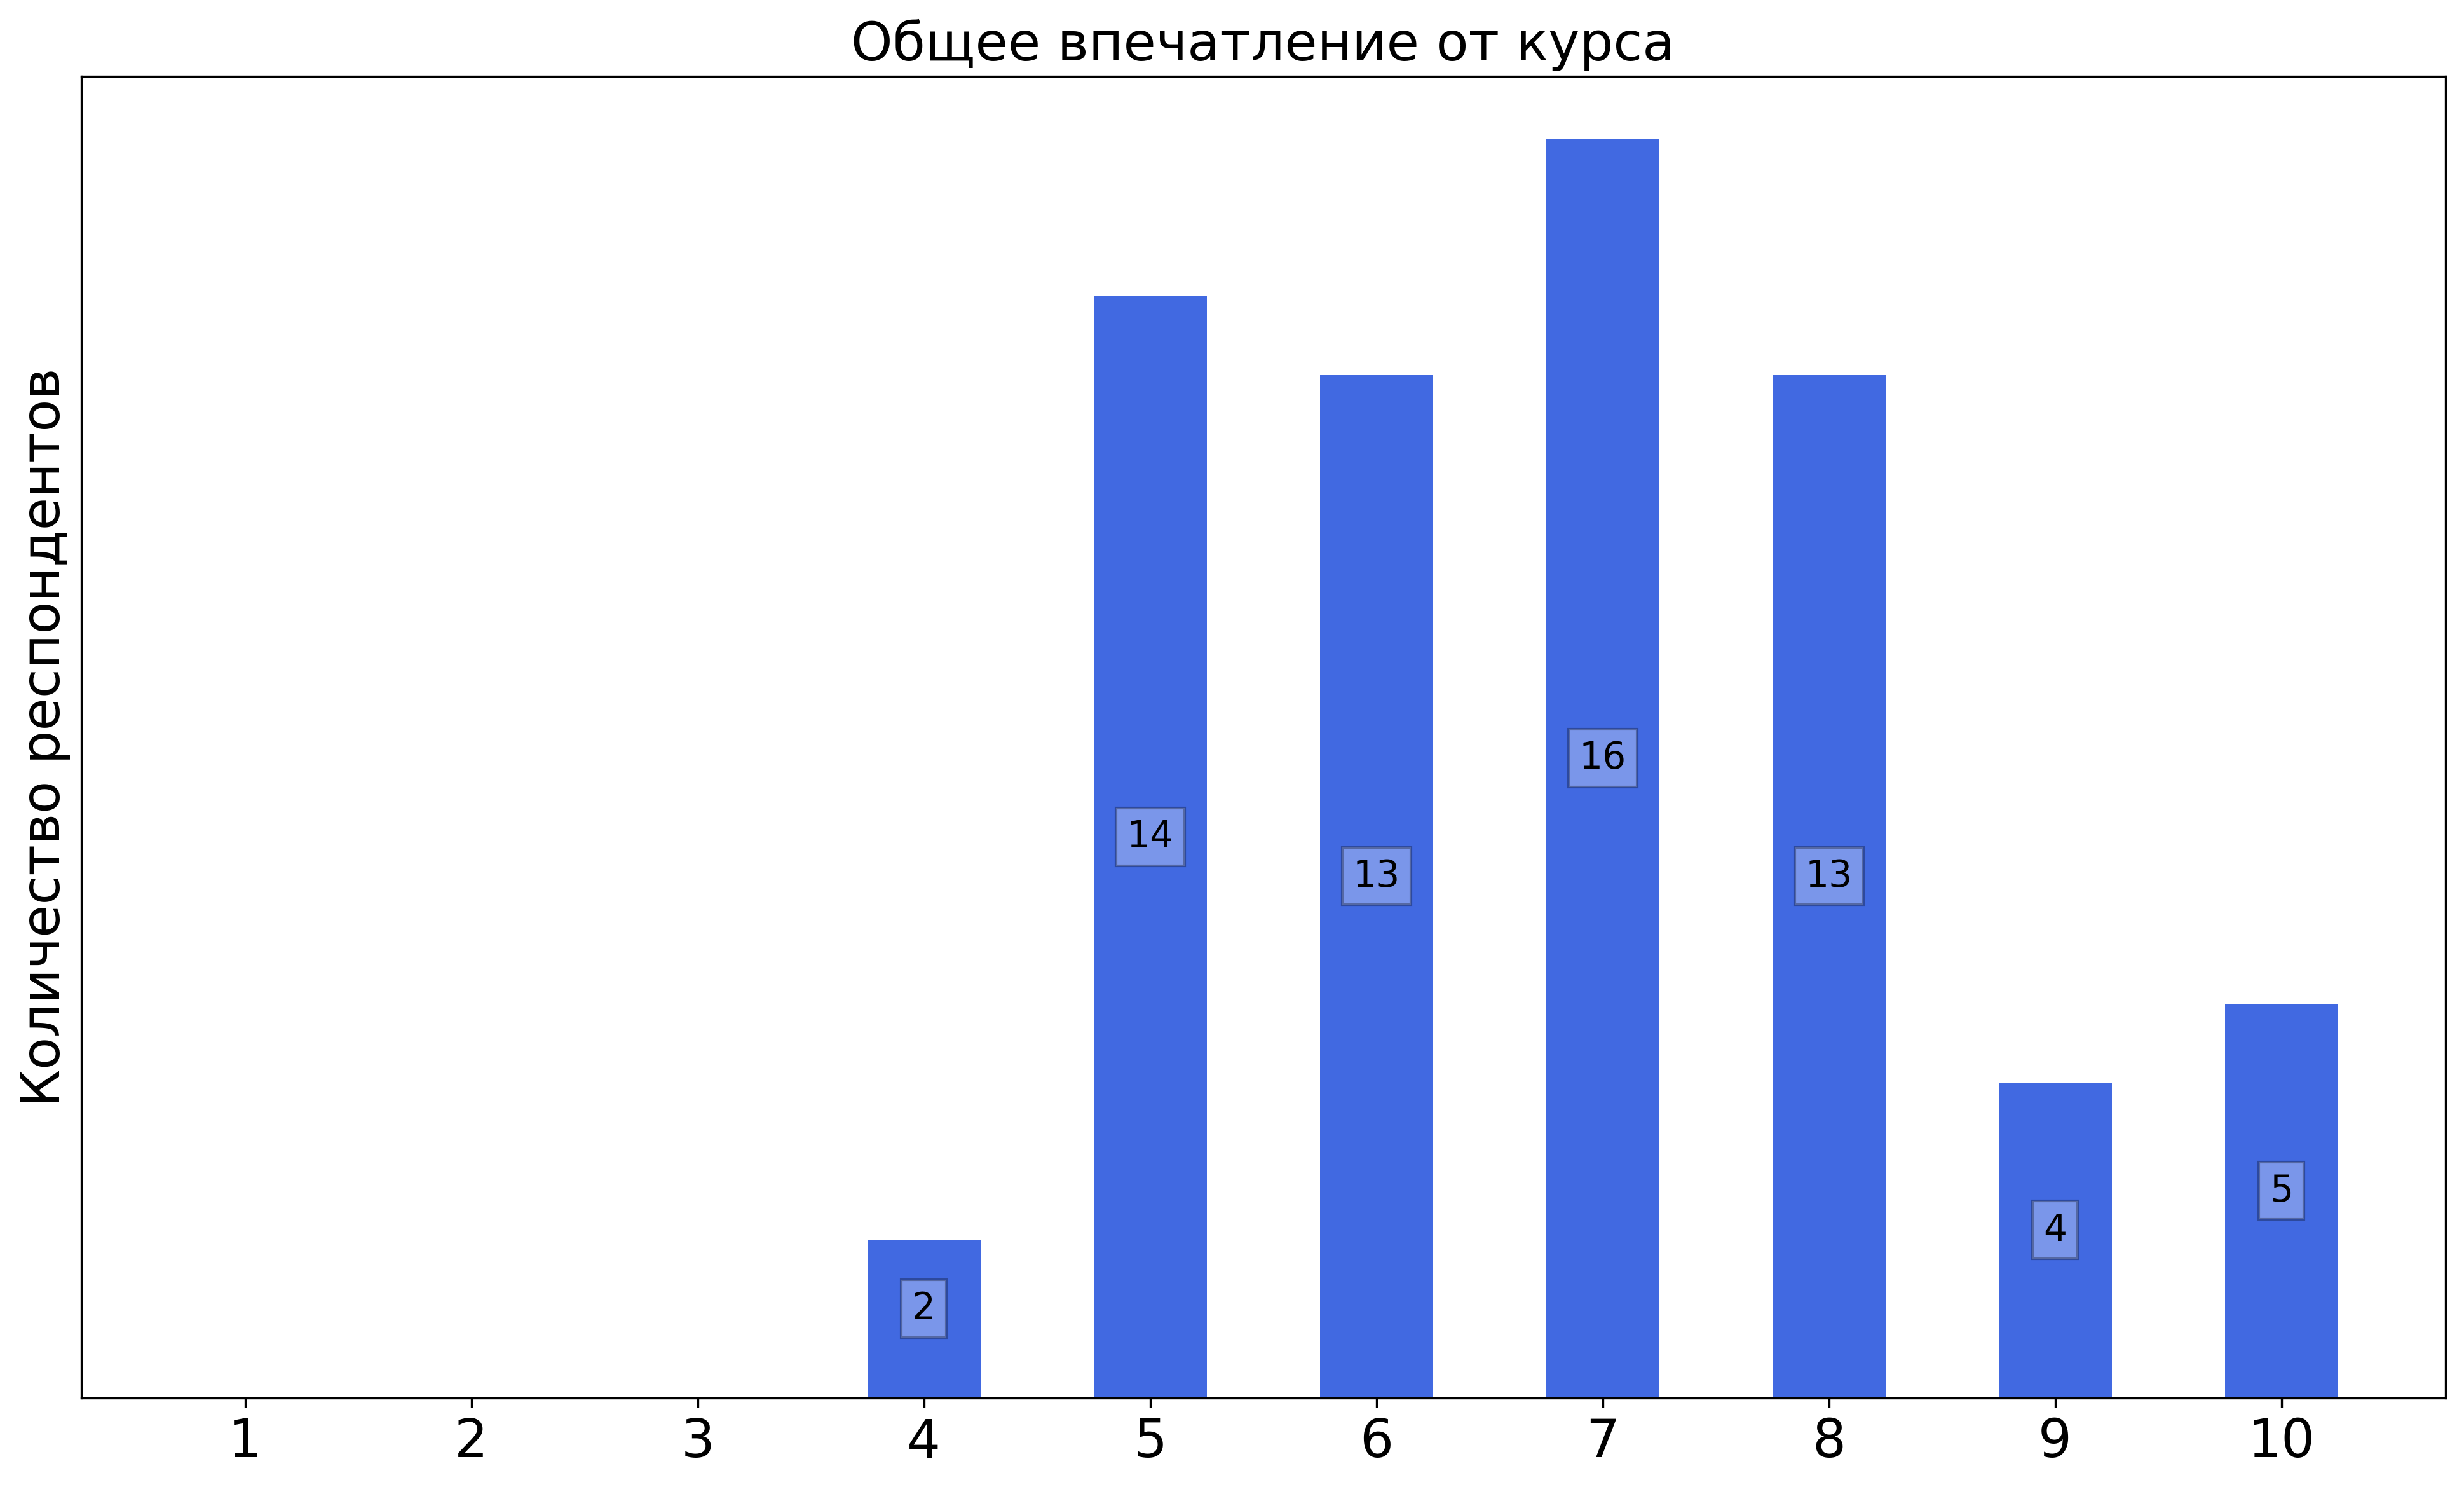
\includegraphics[width=\textwidth]{images/3 course/Вычислительная математика/general-0.png}
			\end{subfigure}
		\end{figure}

	\subsubsection{Материалы, использумые респондентами при изучении курса}

		\begin{figure}[H]
			\centering
			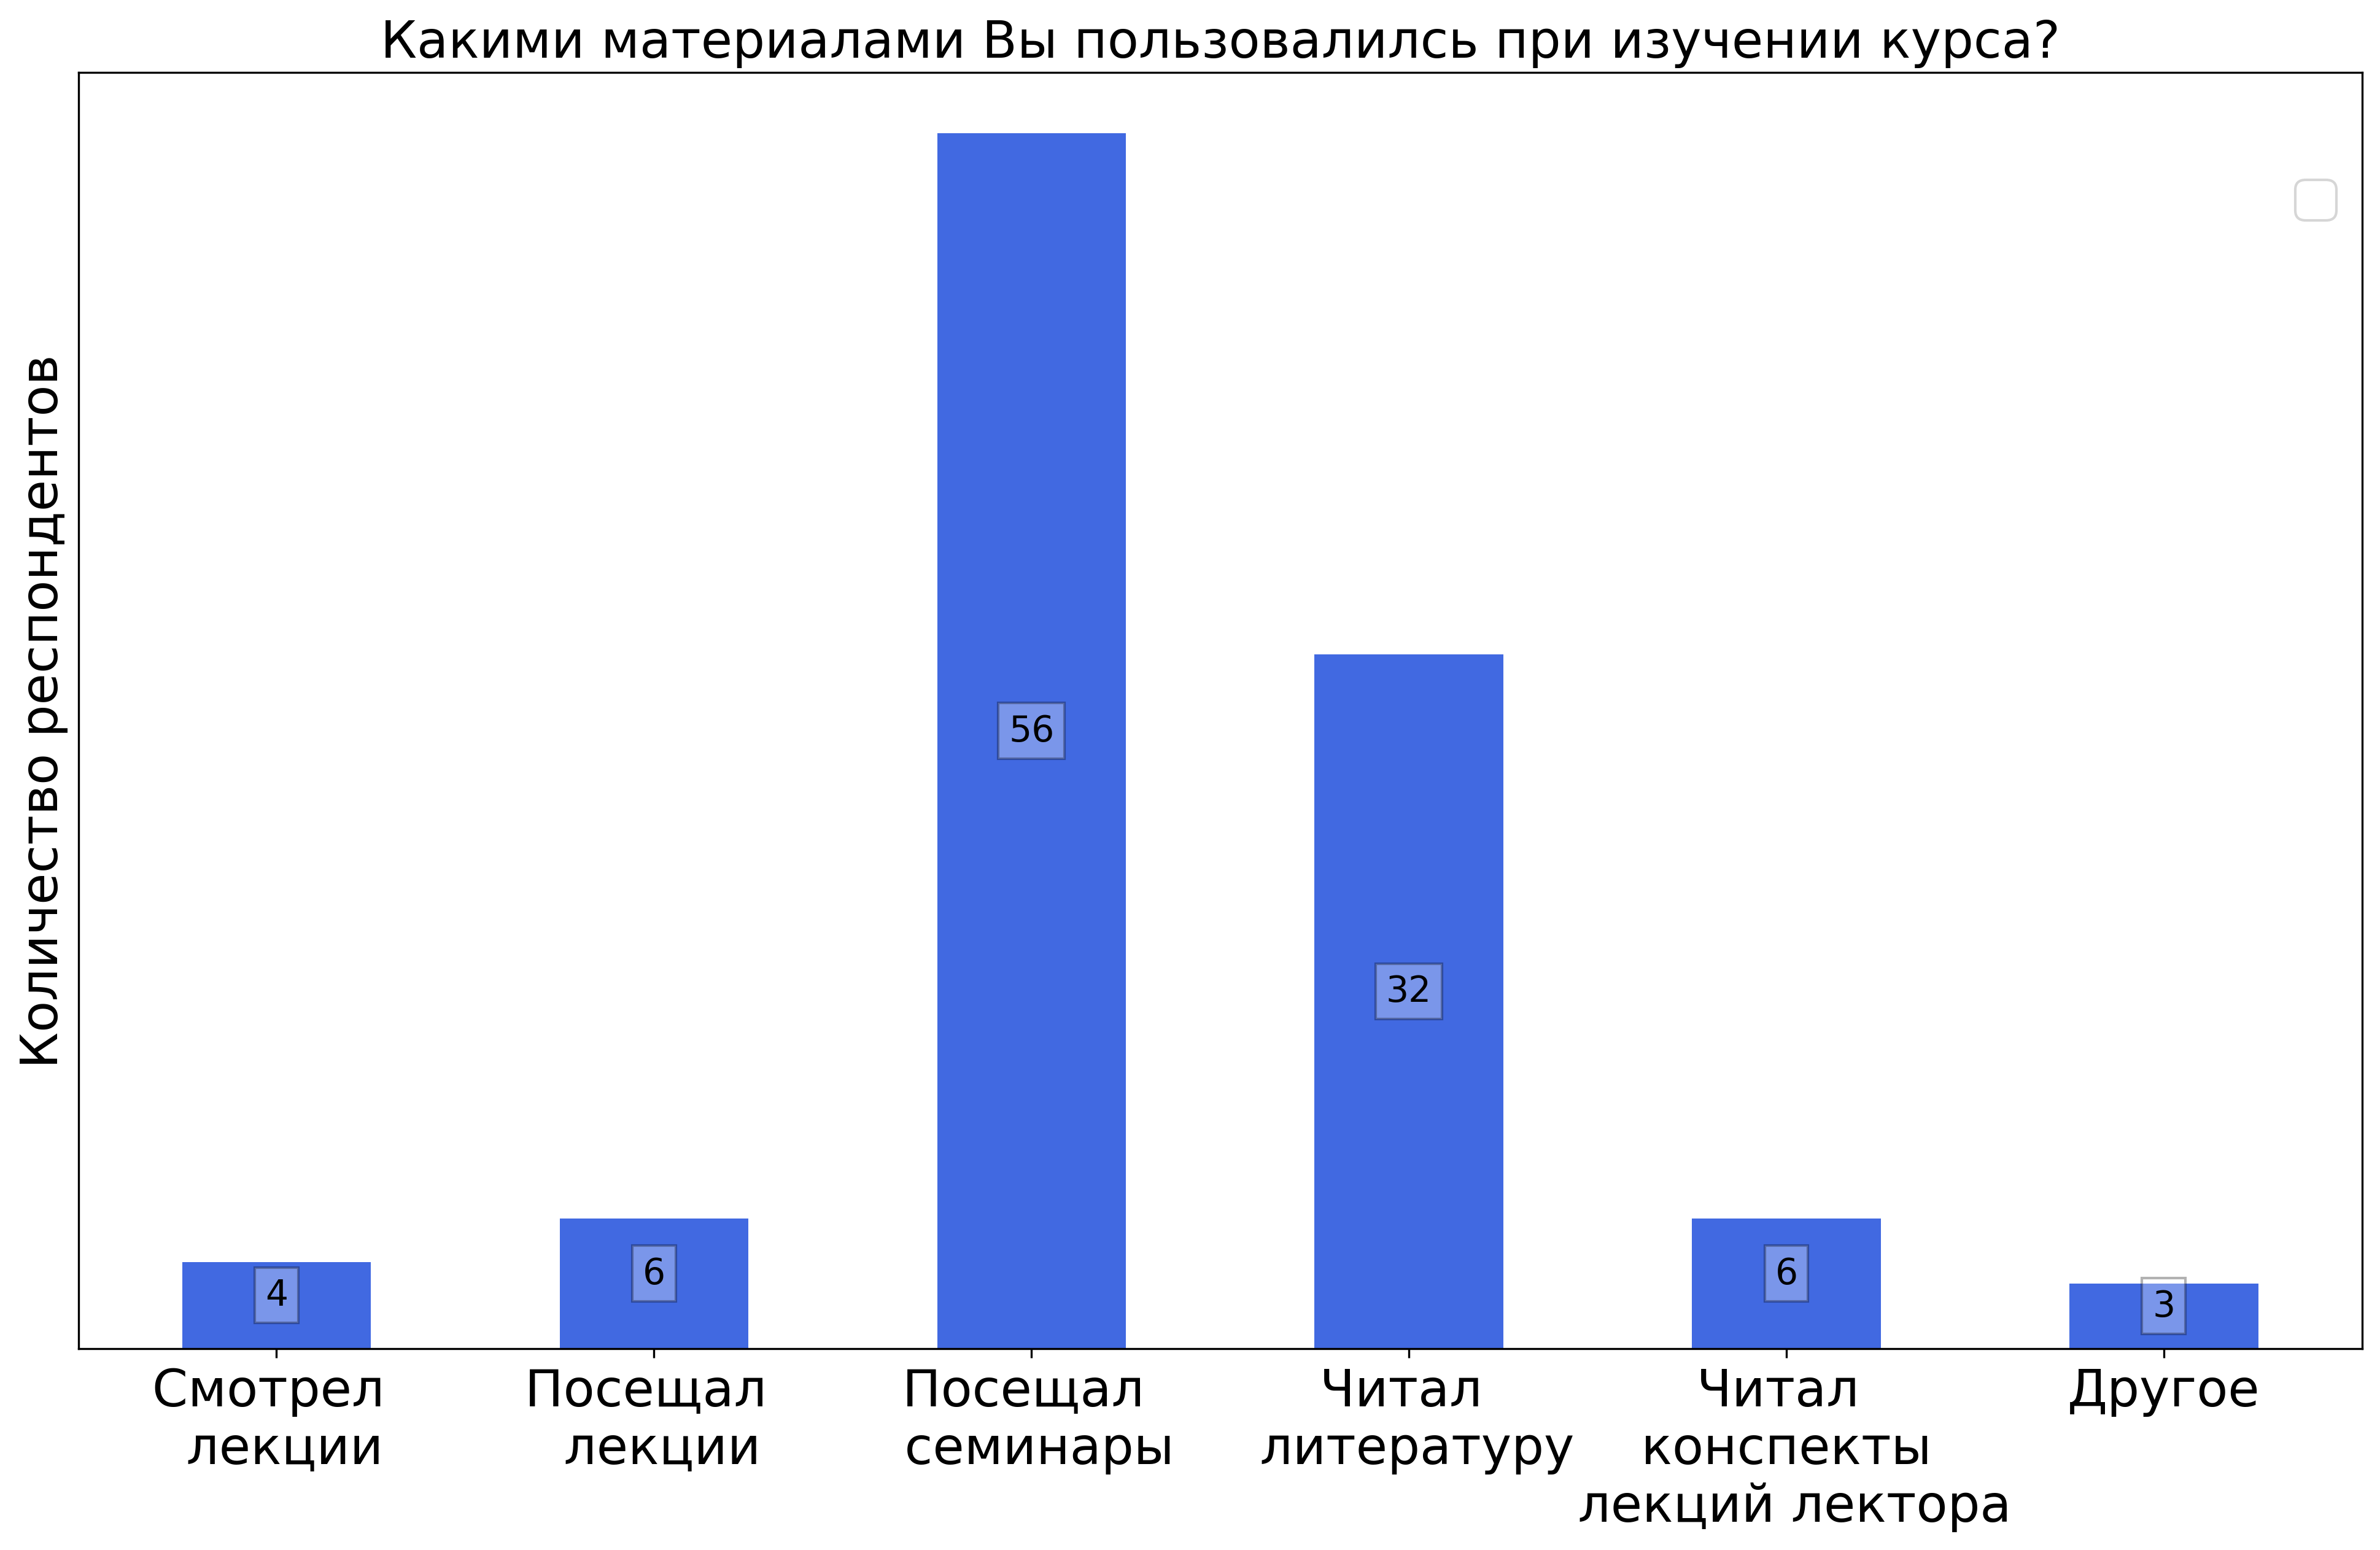
\includegraphics[width = 0.45\textwidth]{images/3 course/Вычислительная математика/materials.png}
		\end{figure}

		\textit{В качестве других источников информации студенты указали:} 
		\begin{itemize}
			\item методички Петрова Михаила Николаевича.
		\end{itemize}

	\subsubsection{Отзыв студентов о лекциях. Лектор: Петров И.Б.}

		\begin{figure}[H]
			\centering
            \begin{subfigure}[b]{0.45\textwidth}
				\centering
				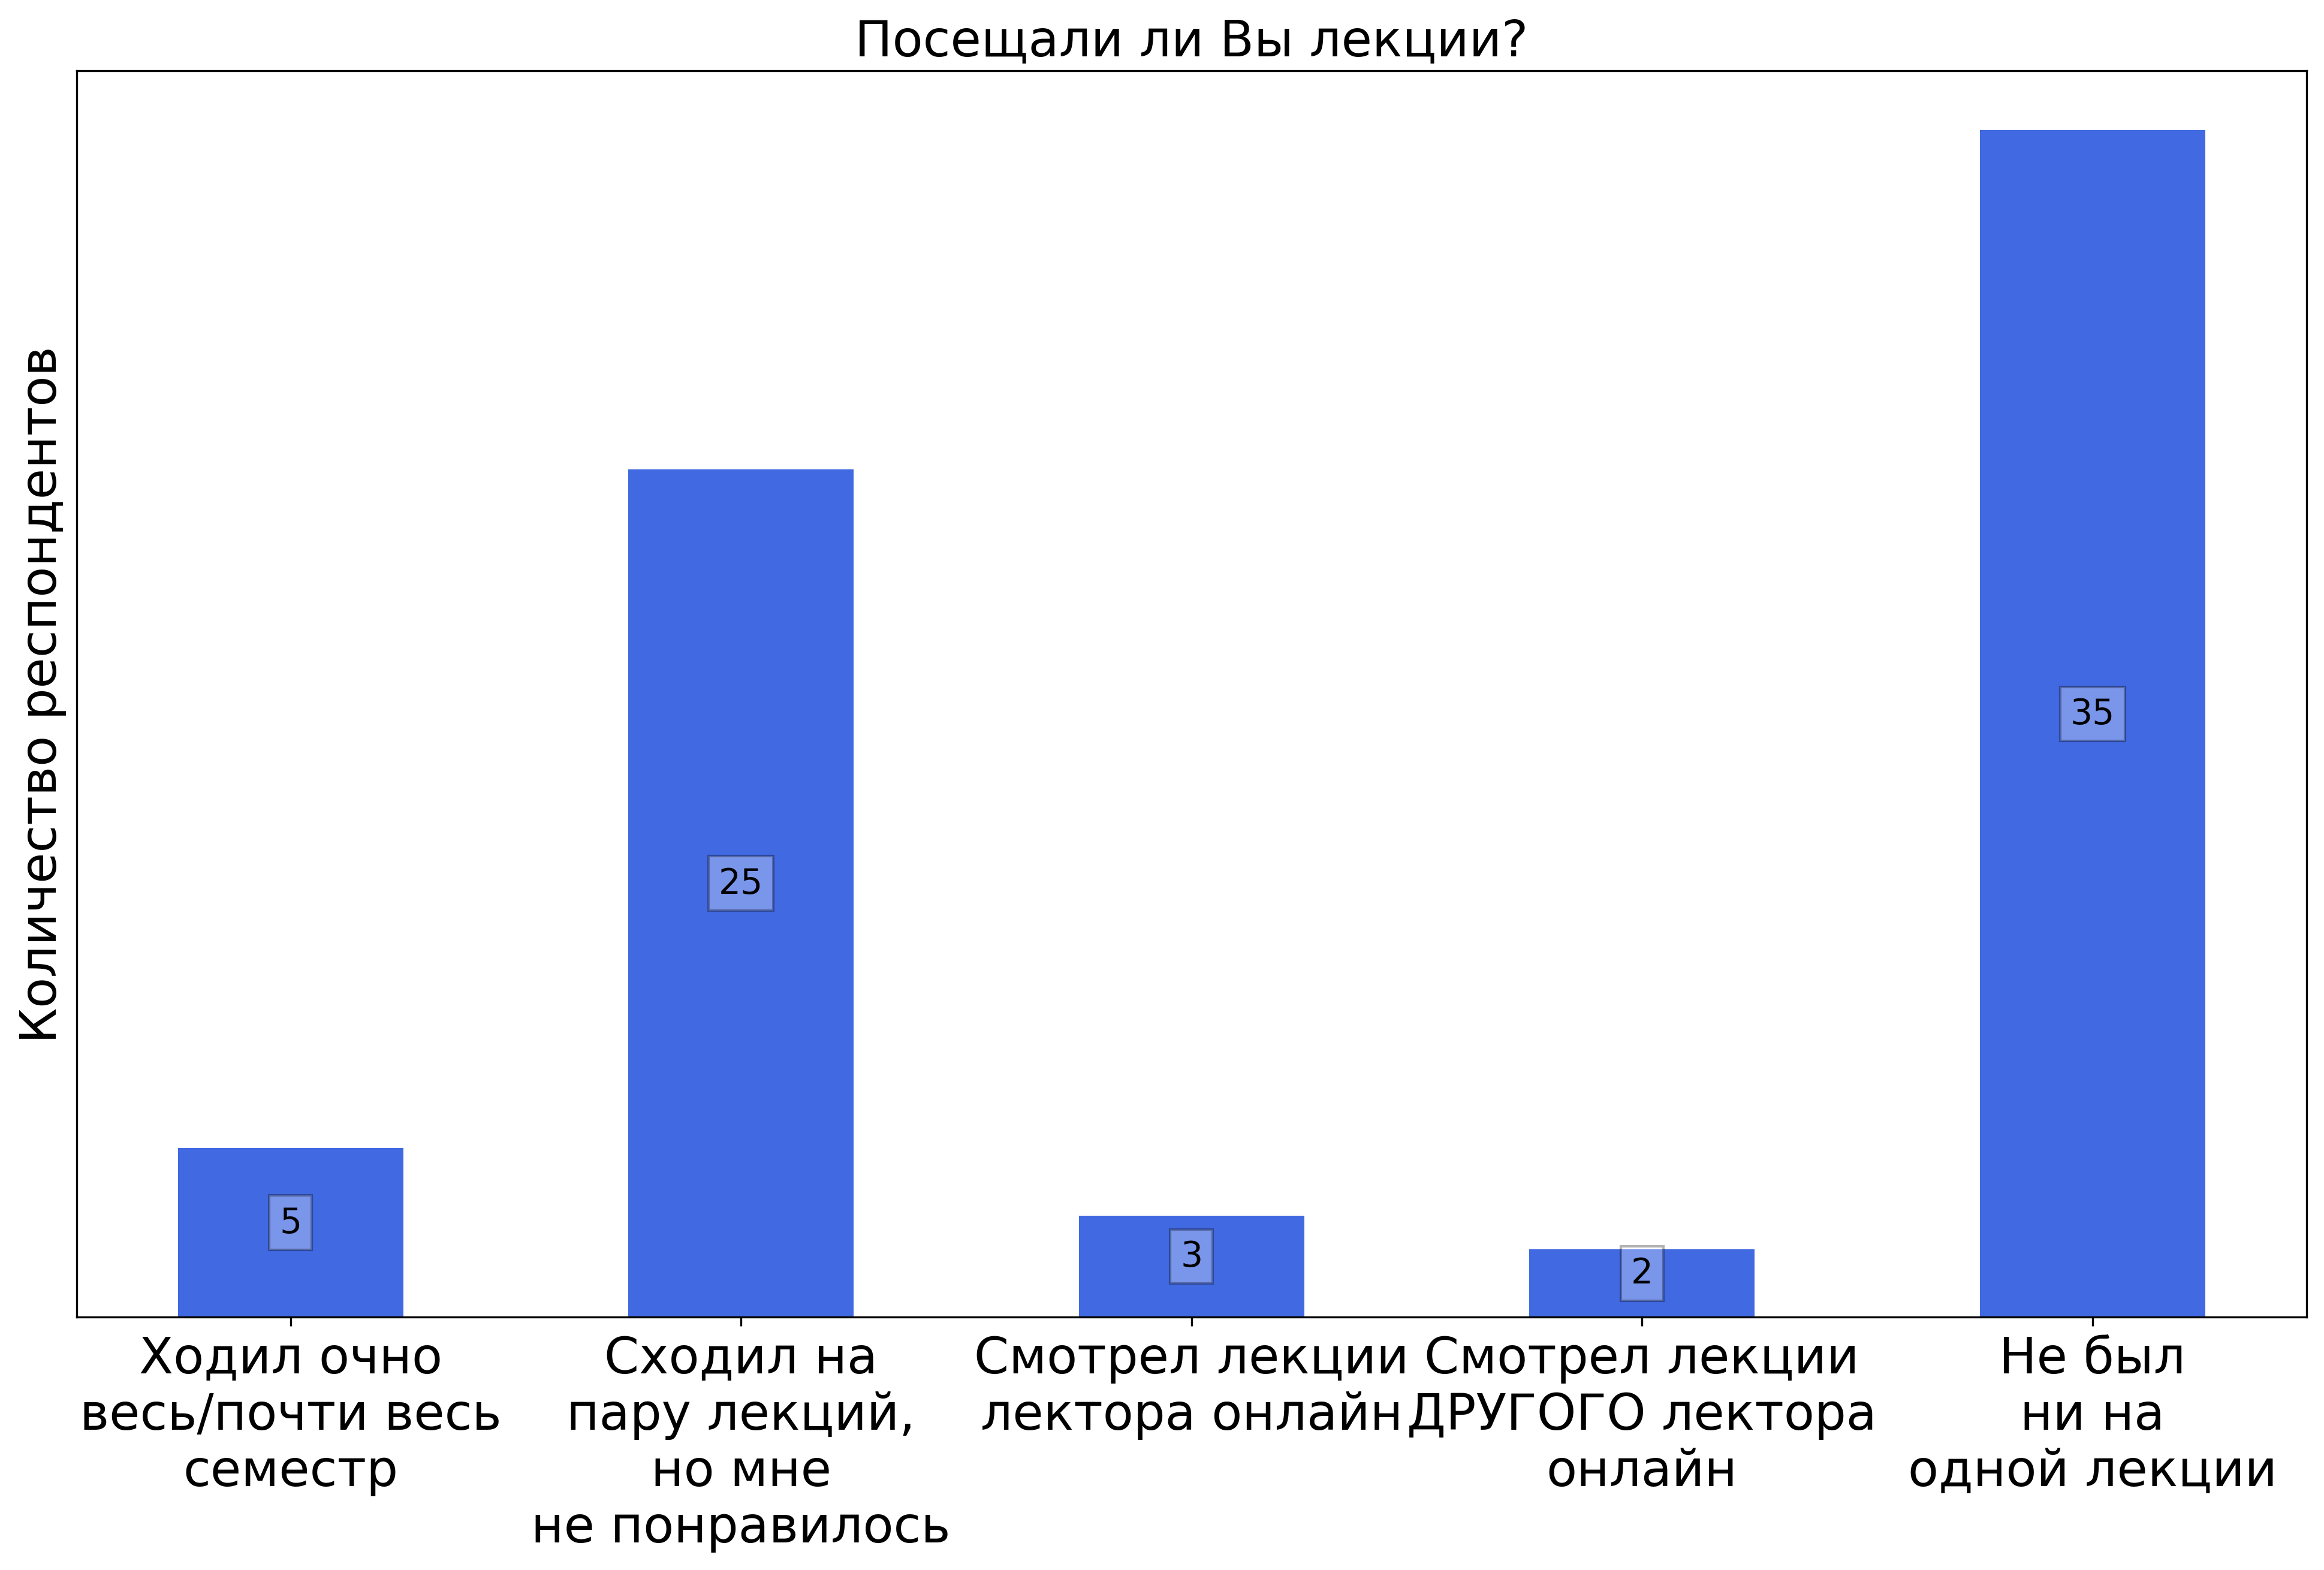
\includegraphics[width=\textwidth]{images/3 course/Вычислительная математика/lecturer-questions-Петров И.Б.-0.png}
			\end{subfigure}
			\begin{subfigure}[b]{0.45\textwidth}
				\centering
				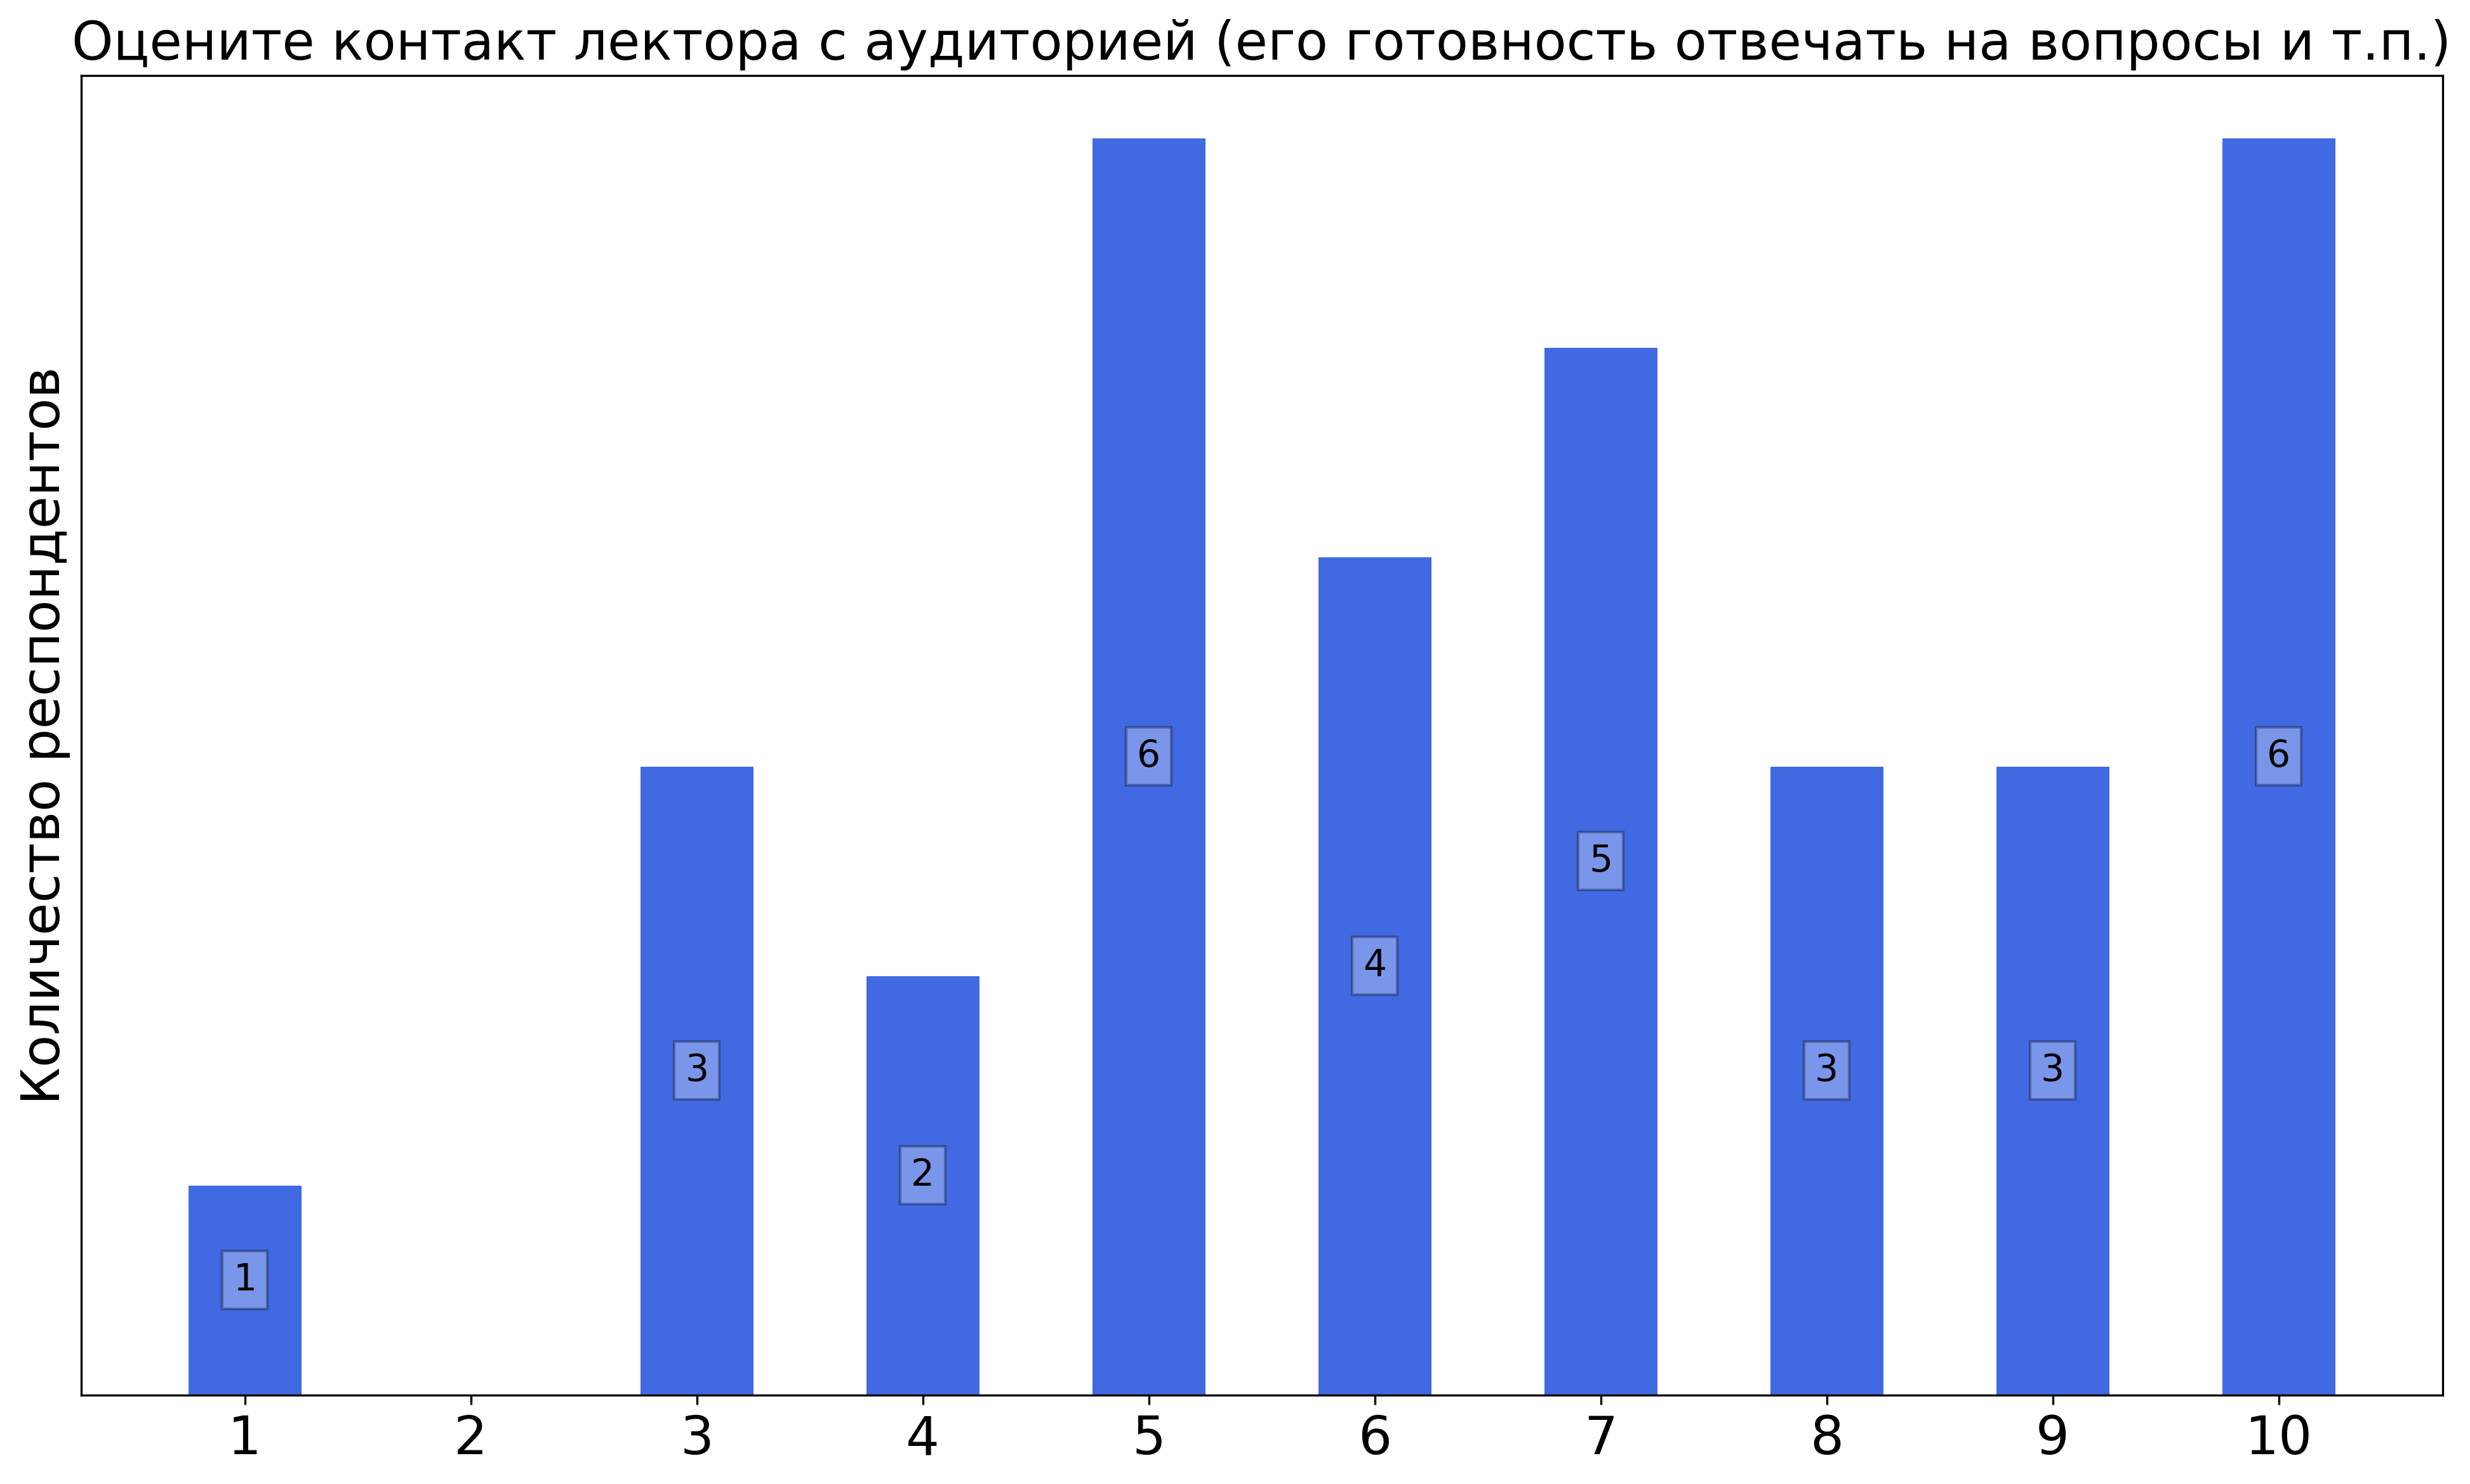
\includegraphics[width=\textwidth]{images/3 course/Вычислительная математика/lecturer-marks-Петров И.Б.-0.png}
			\end{subfigure}
			\begin{subfigure}[b]{0.45\textwidth}
				\centering
				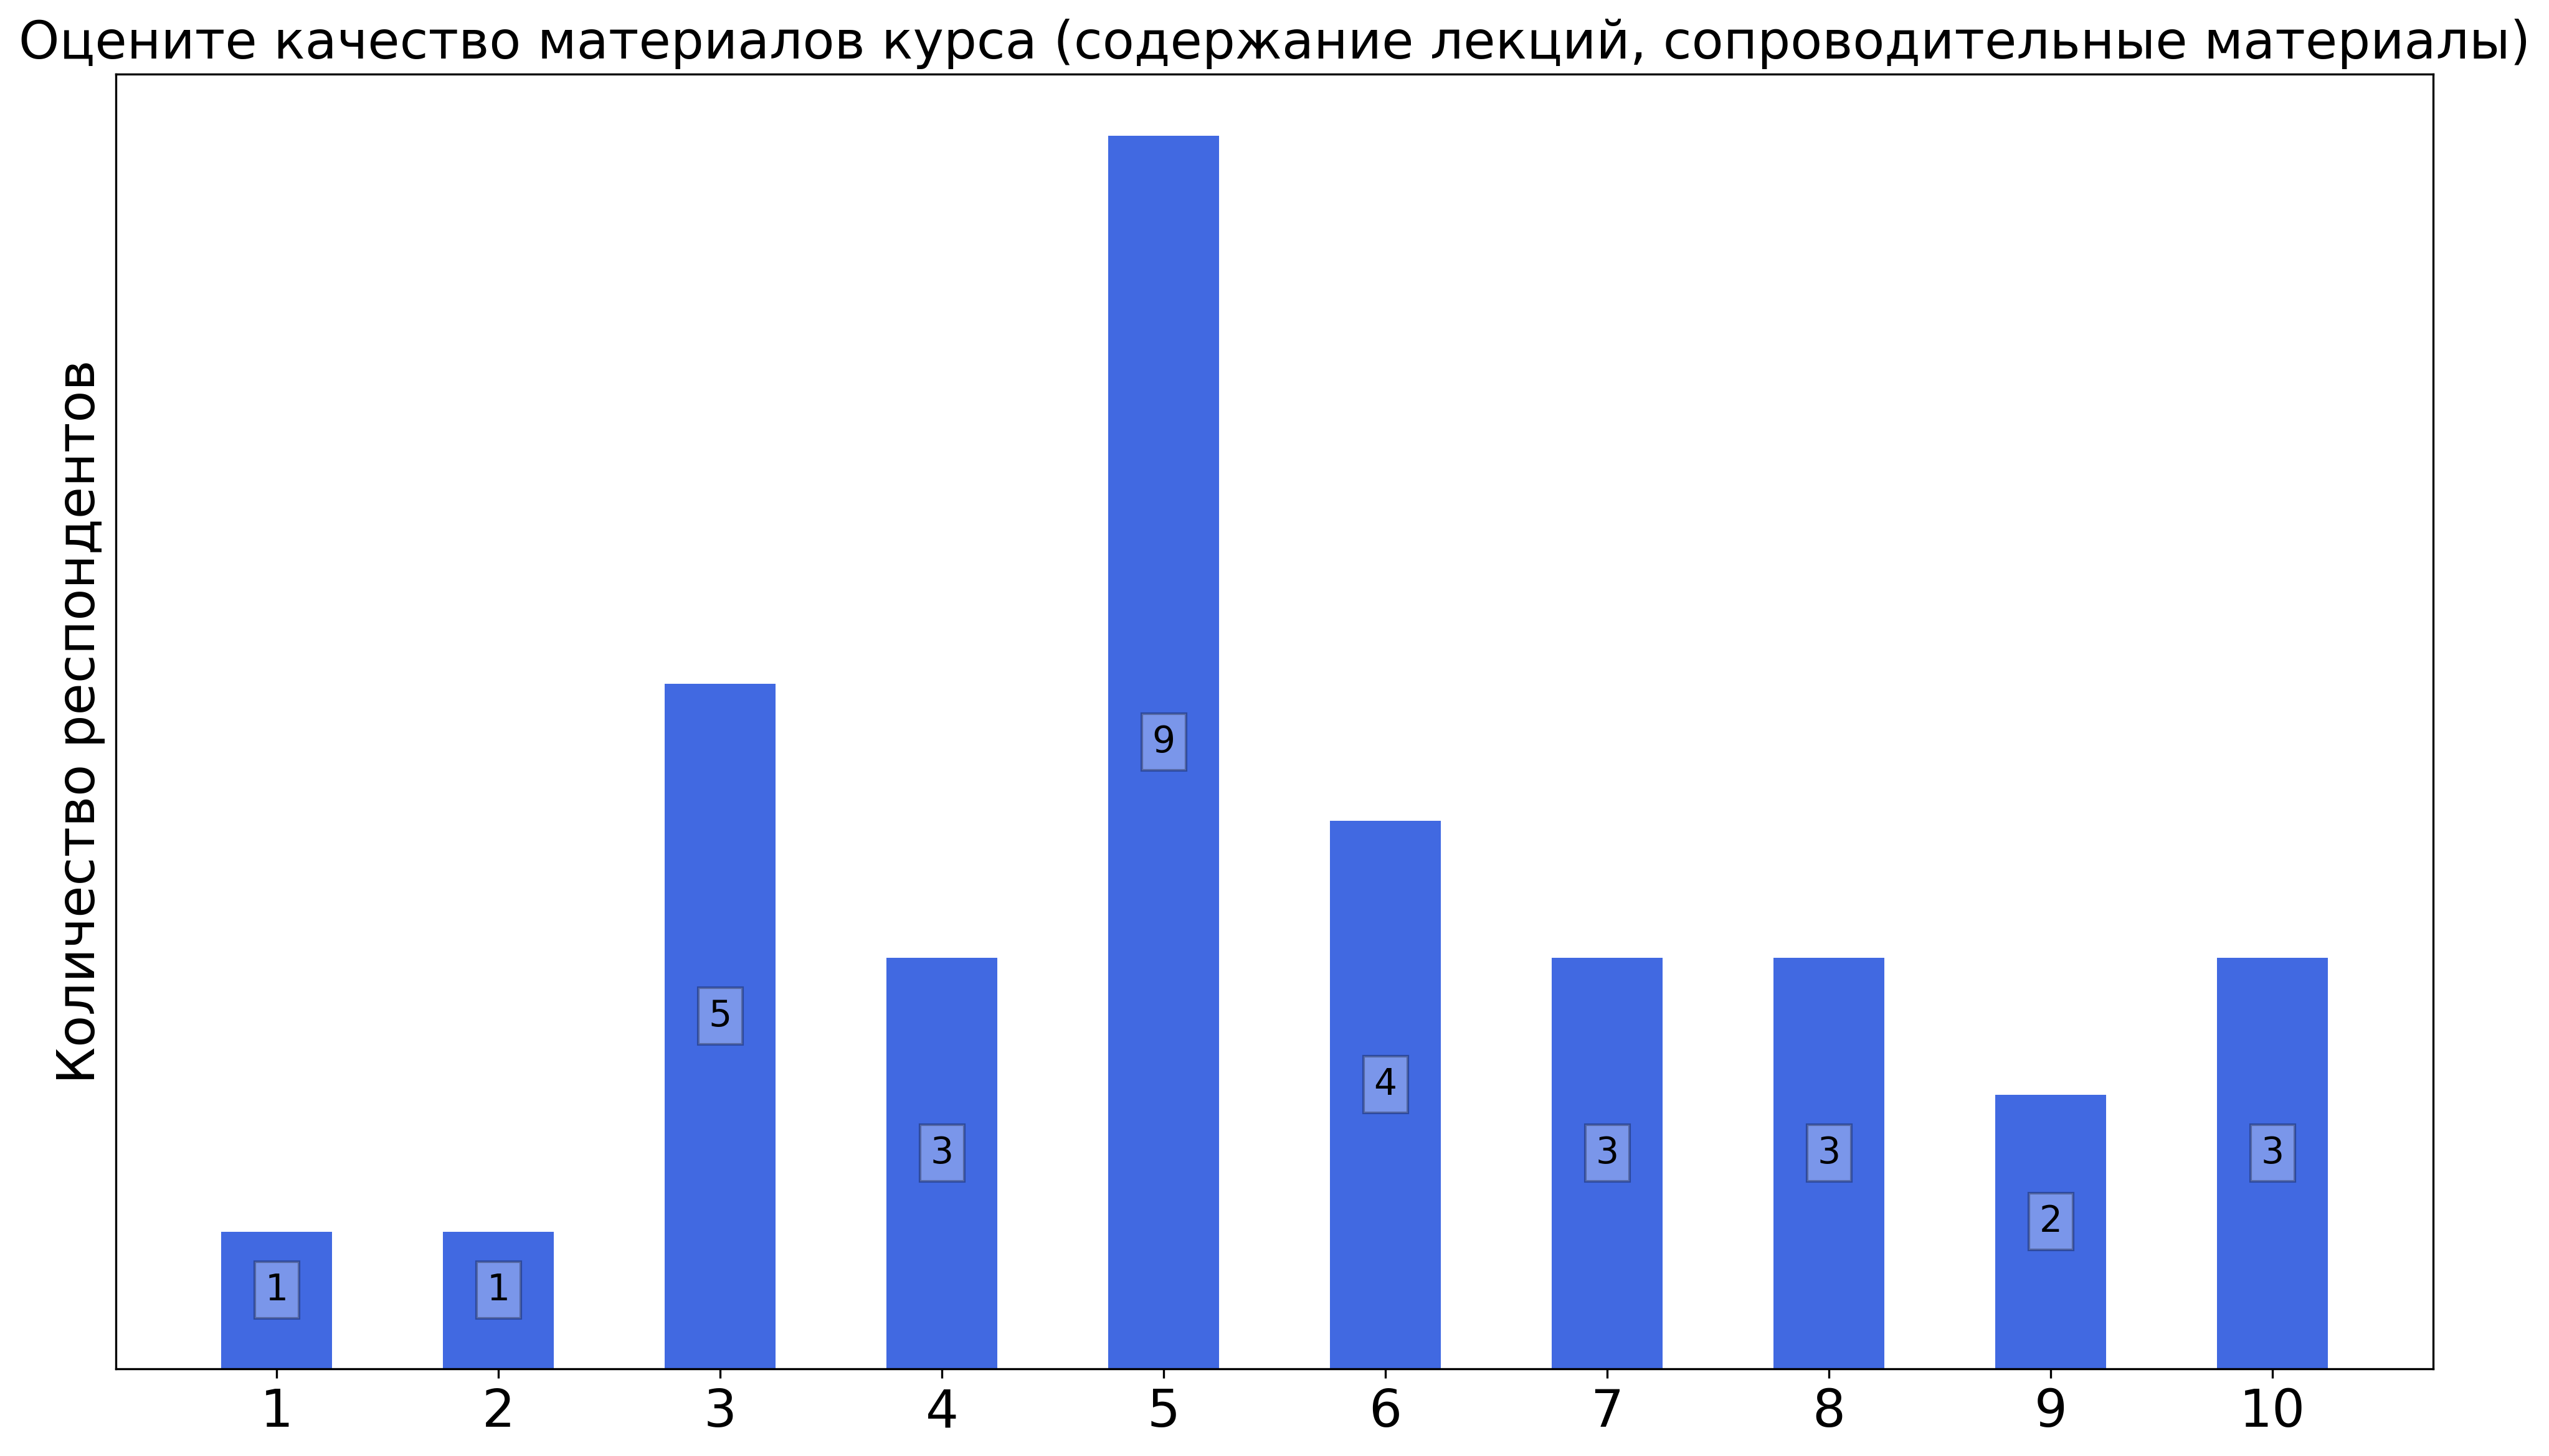
\includegraphics[width=\textwidth]{images/3 course/Вычислительная математика/lecturer-marks-Петров И.Б.-1.png}
			\end{subfigure}
			\begin{subfigure}[b]{0.45\textwidth}
				\centering
				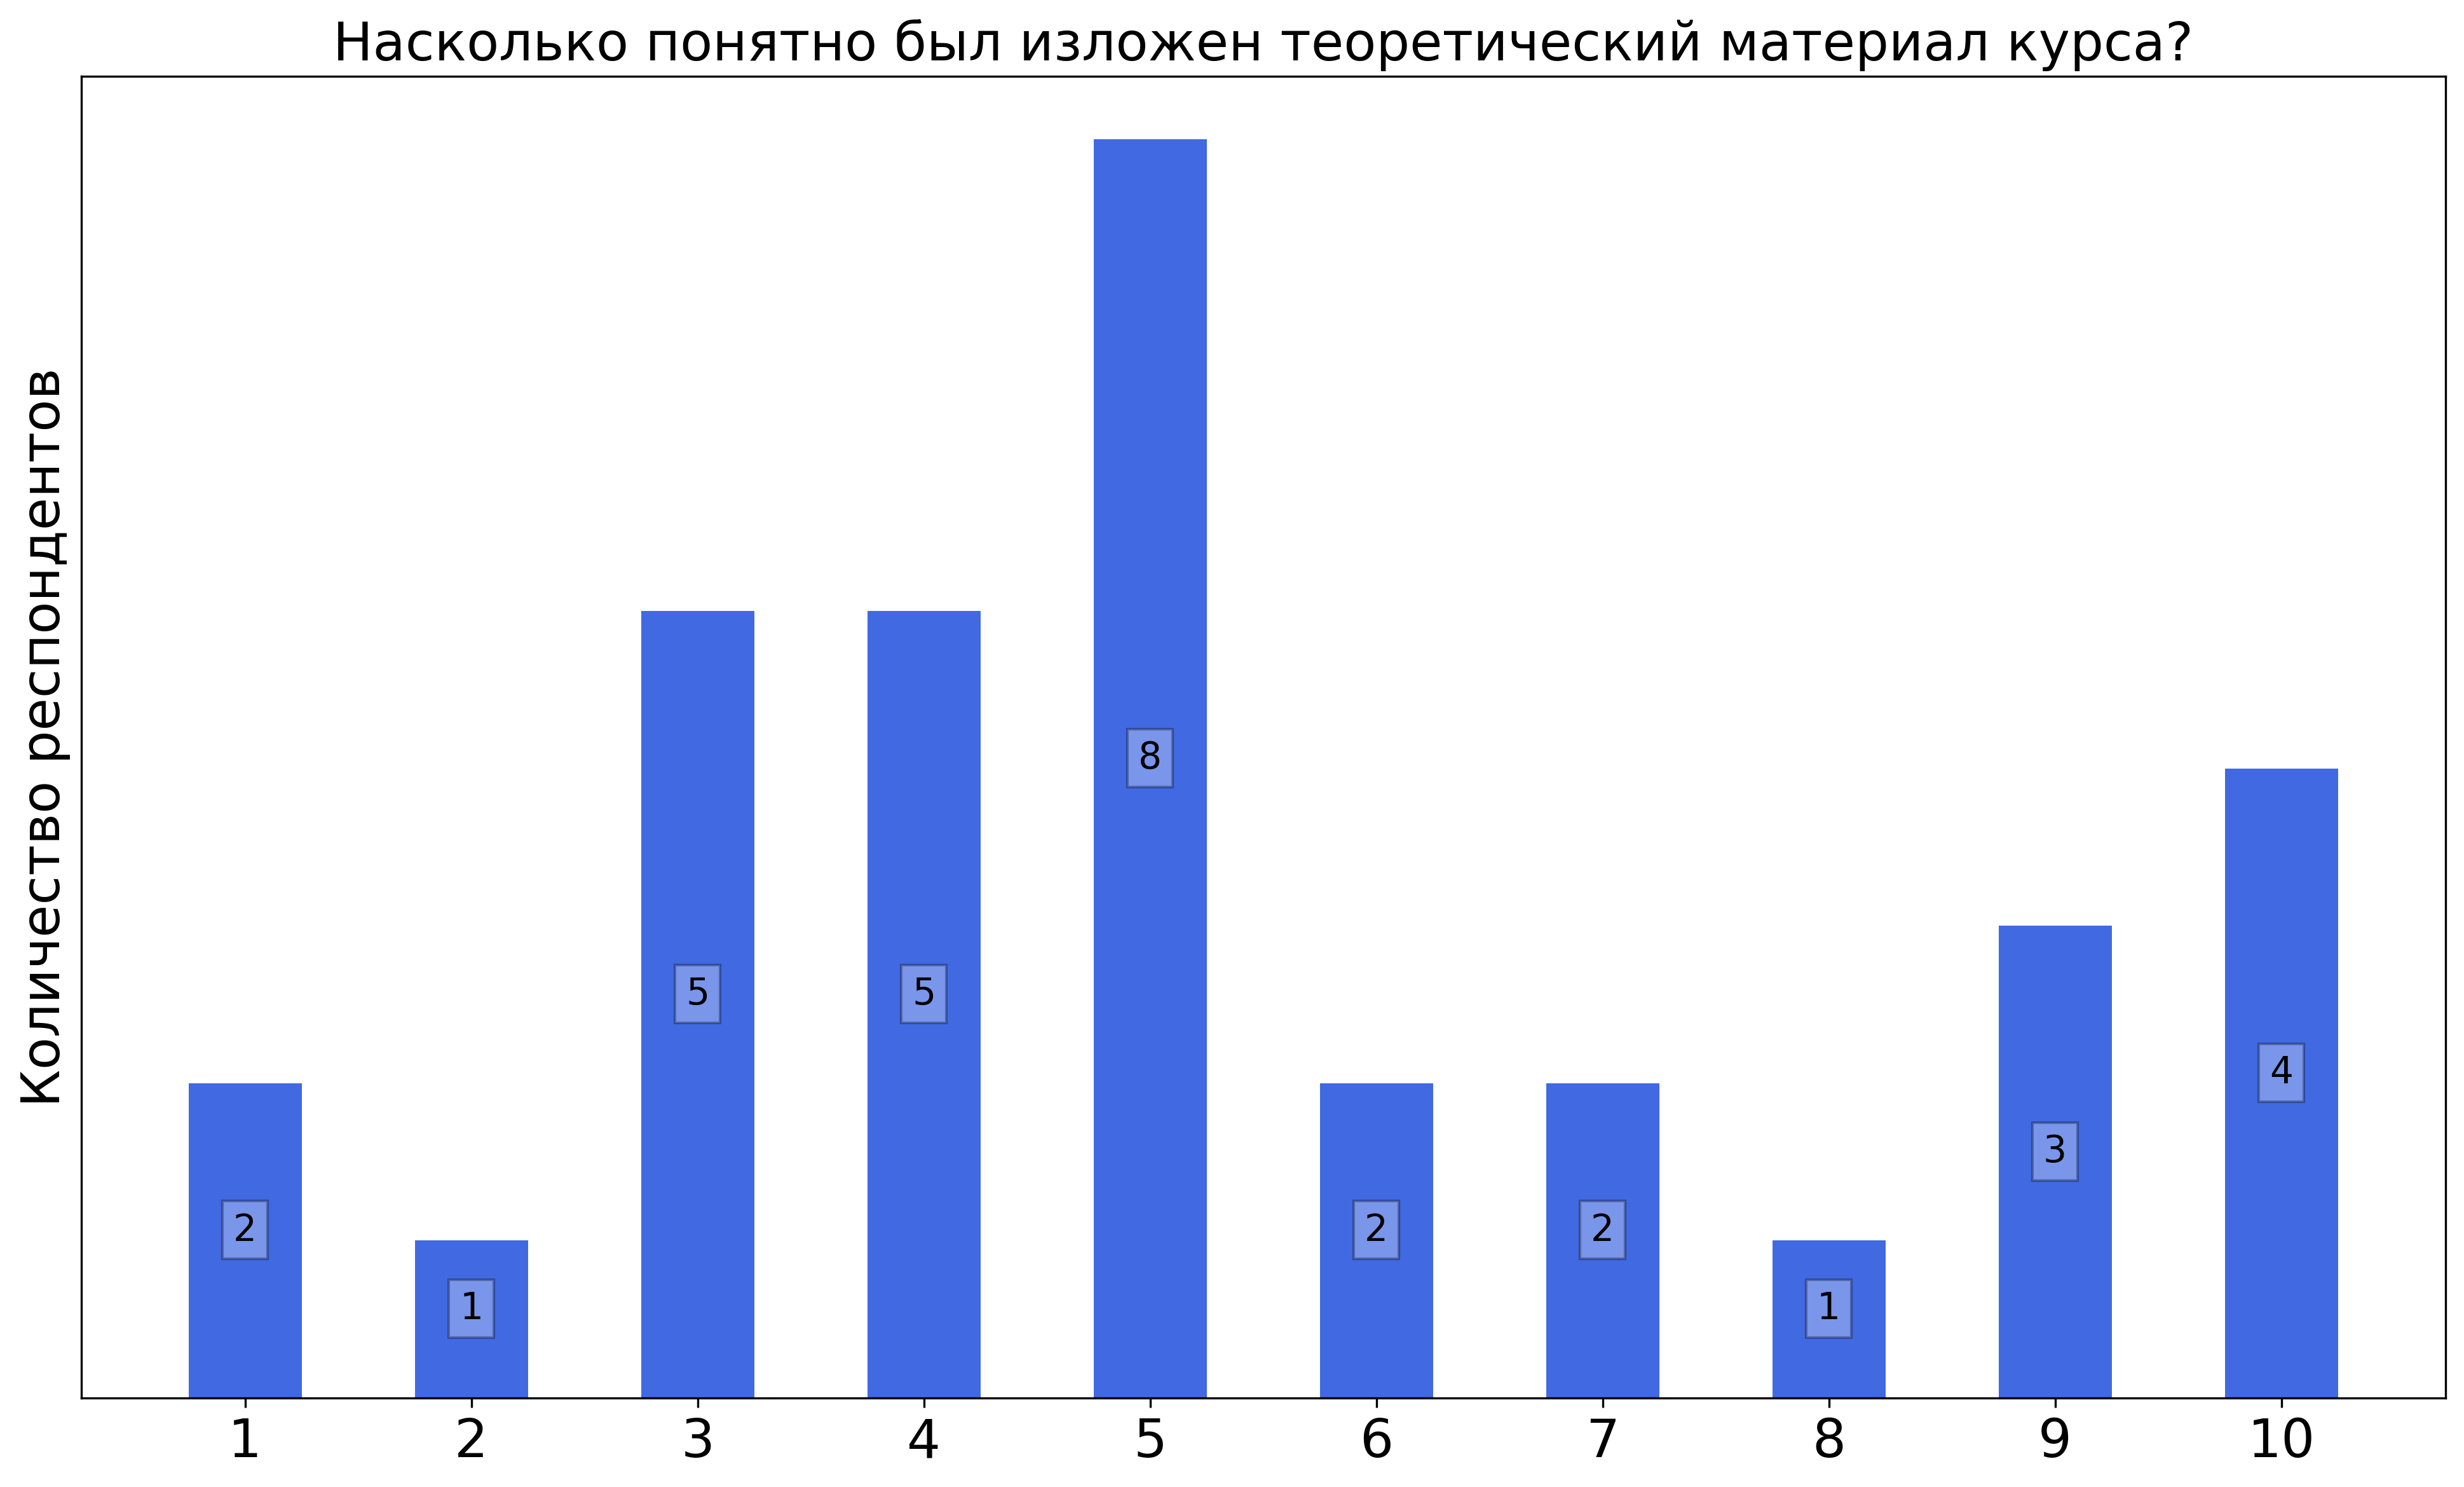
\includegraphics[width=\textwidth]{images/3 course/Вычислительная математика/lecturer-marks-Петров И.Б.-2.png}
			\end{subfigure}	
			\begin{subfigure}[b]{0.45\textwidth}
				\centering
				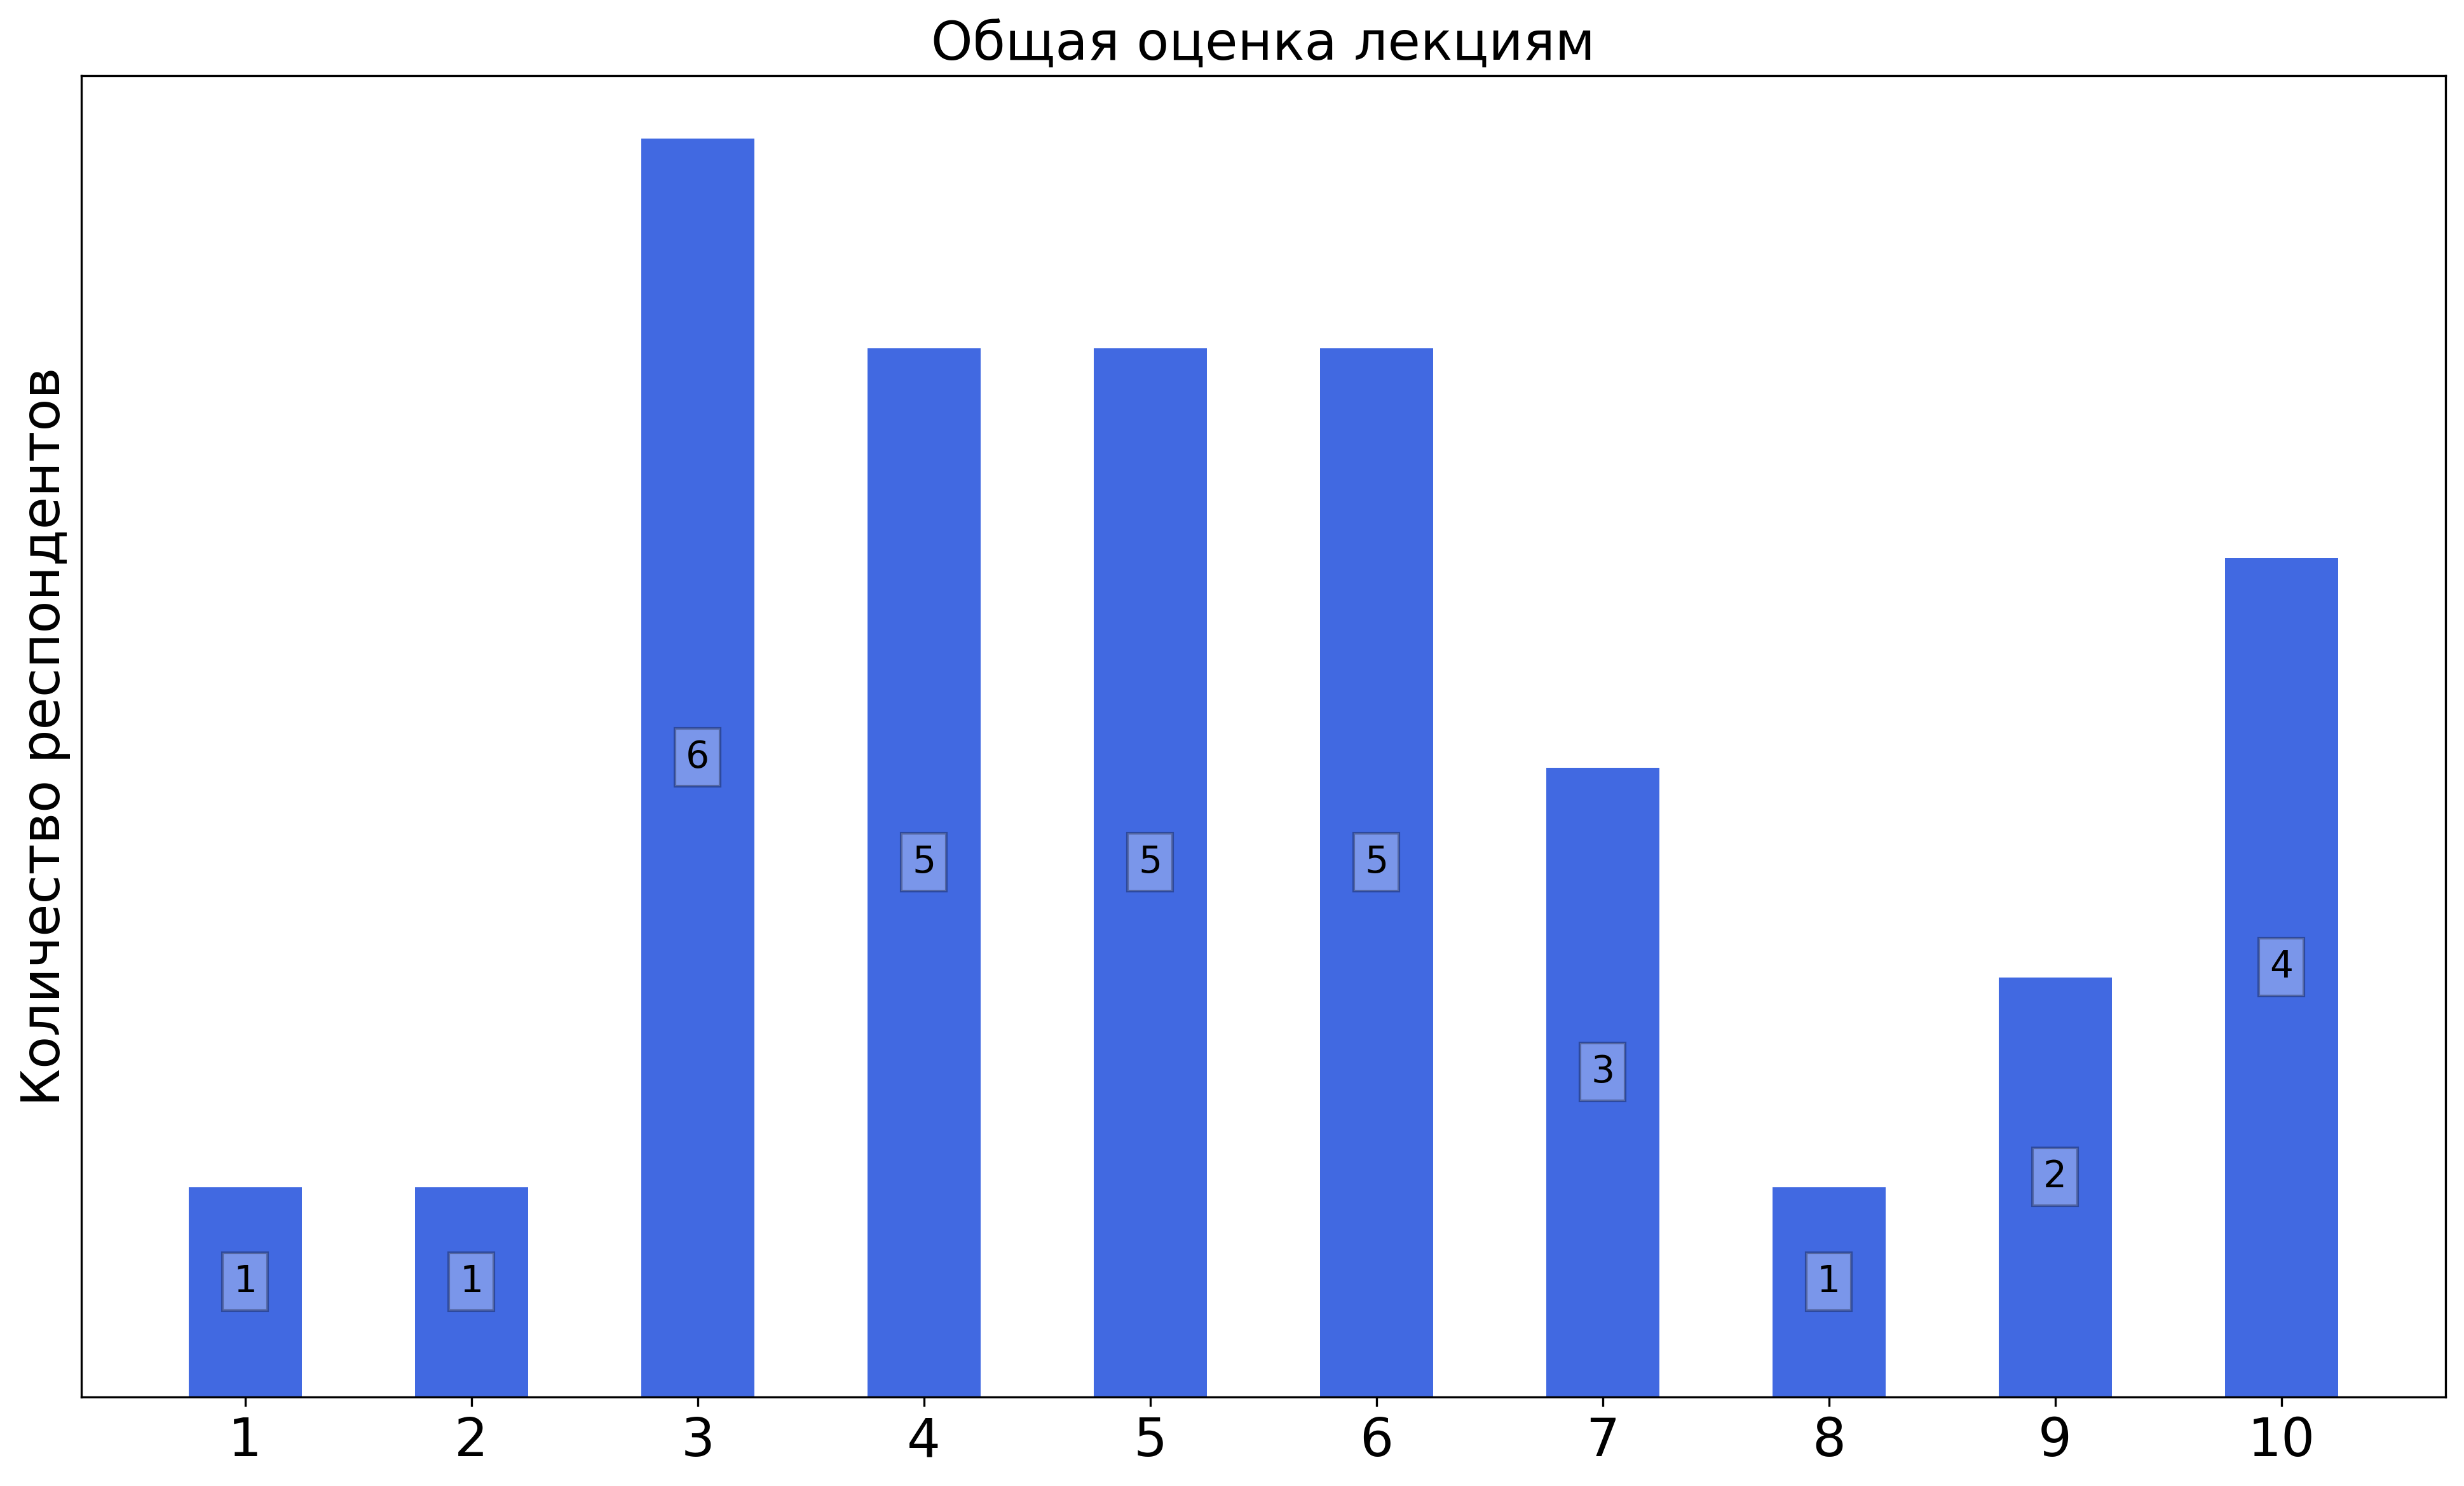
\includegraphics[width=\textwidth]{images/3 course/Вычислительная математика/lecturer-marks-Петров И.Б.-3.png}
			\end{subfigure}
			\caption{Оценки респондентов о качестве преподавания лекций по курсу <<Вычислительная математика>>}
		\end{figure}

		\textbf{Комментарии студентов о лекциях\protect\footnote{сохранены оригинальные орфография и пунктуация}}
            \begin{commentbox} 
                Лекции  воспринимаются очень тяжело, так как читаются по презентациям. Невозможно успеть просто все записать, на осознание времени нет совсем. Поэтому лекции превращаются в перечисление набора фактов, в котором либо я не смог усмотреть какой-то глубины, либо ее там просто нет. В целом самое красивое часто остается за кадром, и вычматы стали казаться очень душным и устаревшим предметом. Надо отметить, что лектор рассказывает так же историю появления некоторых методов, и примеры реального применения, это классно, но основные проблемы остаются. На вопросы лектор отвечает, но часто ответ немного не соответствует вопросу и просто повторяет уже сказанное на лекции. 
            \end{commentbox} 
        
            \begin{commentbox} 
                Конспекты было сложно вести из-за темпа лекции. Материал тоже не очень понятно излагался. Забавно, но я даже не могу объяснить, почему, я, в отличие от других предетов, просто не понимал, что происходит 
            \end{commentbox} 
        
            \begin{commentbox} 
                Просто презентации, не успевал ничего записывать и не было какой-то понятной структуры 
            \end{commentbox} 
        
            \begin{commentbox} 
                Сходил на две лекции, показались весьма бесполезными. Из теории было достаточно того, что дают на семинарах. Мне показалось, что лекции по вычислительной математике - самая бесполезная вещь 
            \end{commentbox} 
        
            \begin{commentbox} 
                Лекции в лучшем случае повторяют материал семинарских занятий, изложение хотелось бы перестроить ближе к рамкам лекций по информатике/математике, сейчас лекционный курс выглядит сырым 
            \end{commentbox} 
        
            \begin{commentbox} 
                считаю, что этому предмету лекции абсолютно не нужны, семинаров/лабораторных работ более чем достаточно 
            \end{commentbox} 
        
            \begin{commentbox} 
                С первого же захода не понравились лекции. Первую половину лекции вообще была история, потом тоже не очень понятный материал, так еще и в виде презентаций (что ухудшает читабельность выкладок). Приходил после еще раз в середине семестра - замечания остались те же.  Также не нравится структура лекций - возникло ощущения, что мы с ничего просто вводим новый метод вычисления. А так лектор шарящий, на вопросы вроде отвечает 
            \end{commentbox} 
        
            \begin{commentbox} 
                Символы на слайдах презентации часто съезжали в сторону, что затрудняло понимание материала. 
            \end{commentbox} 
        
            \begin{commentbox} 
                Вещает не очень понятно, воспринимать математический предмет с презентации очень сложно 
            \end{commentbox} 
        
            \begin{commentbox} 
                Лично для меня тяжело воспринимается материал по математической дисциплине, который преподносится в виде презентаций. Последовательное изложение на доске позволяет разобраться в теме, в отличии от презентаций.  
            \end{commentbox} 
        
            \begin{commentbox} 
                Не понравилось, лекции преподаются кое-как 
            \end{commentbox} 
        
            \begin{commentbox} 
                Петров И. Б. в буквальном смысле "читвет" лекции с презентации. И делает это так, что студент не успевает ни записать, ни понять то, что говорит лектор. На доске пишет крайне редко и поясняет так себе. Ладно бы просто не всё понятно, что-то не записал - но презентации лектор никуда не выкладывает и не делится. А так как имеется книга Петрова по вычматам, то смысл посещать подобные лекции теряется. 
            \end{commentbox} 
        
            \begin{commentbox} 
                Сами по себе лекции читаются нормально, но толку от них для большинства нет совсем. Излишняя теоретизированность прикладного курса, которая только отнимает лишнее время 
            \end{commentbox} 
        
            \begin{commentbox} 
                Большая проблема лекций по вычислительной математике состоит в том, что они читаются по презентациям и очень бегло, к тому же включая в себя доказательства теорем, не имеющие никакого практического применения. В моём случае курс лекций был попросту не нужен для освоения предмета, все необходимые материалы на различные источники скидывал семинарист. 
            \end{commentbox} 
        
            \begin{commentbox} 
                Мне не понравилось на 1ой лекции, после этого не ходил. Не могу дать оценку преподавательским качествам лектора, но могу сказать, что говорит он тихо и непонятно - это и не понравилось 
            \end{commentbox} 
        
            \begin{commentbox} 
                Не понятно, нужны ли лекции по предмету, может больше практики 
            \end{commentbox} 
        
            \begin{commentbox} 
                Трудно сказать, посетила только одну лекцию 
            \end{commentbox} 
        
            \begin{commentbox} 
                Предмет непонятно зачем, с плохой структуированностью и материалами 
            \end{commentbox} 
    
    
    \subsubsection{Отзыв студентов о семинарах. Семинарист: Кожемяченко А.А.}
		\begin{figure}[H]
			\centering
			\begin{subfigure}[b]{0.45\textwidth}
				\centering
				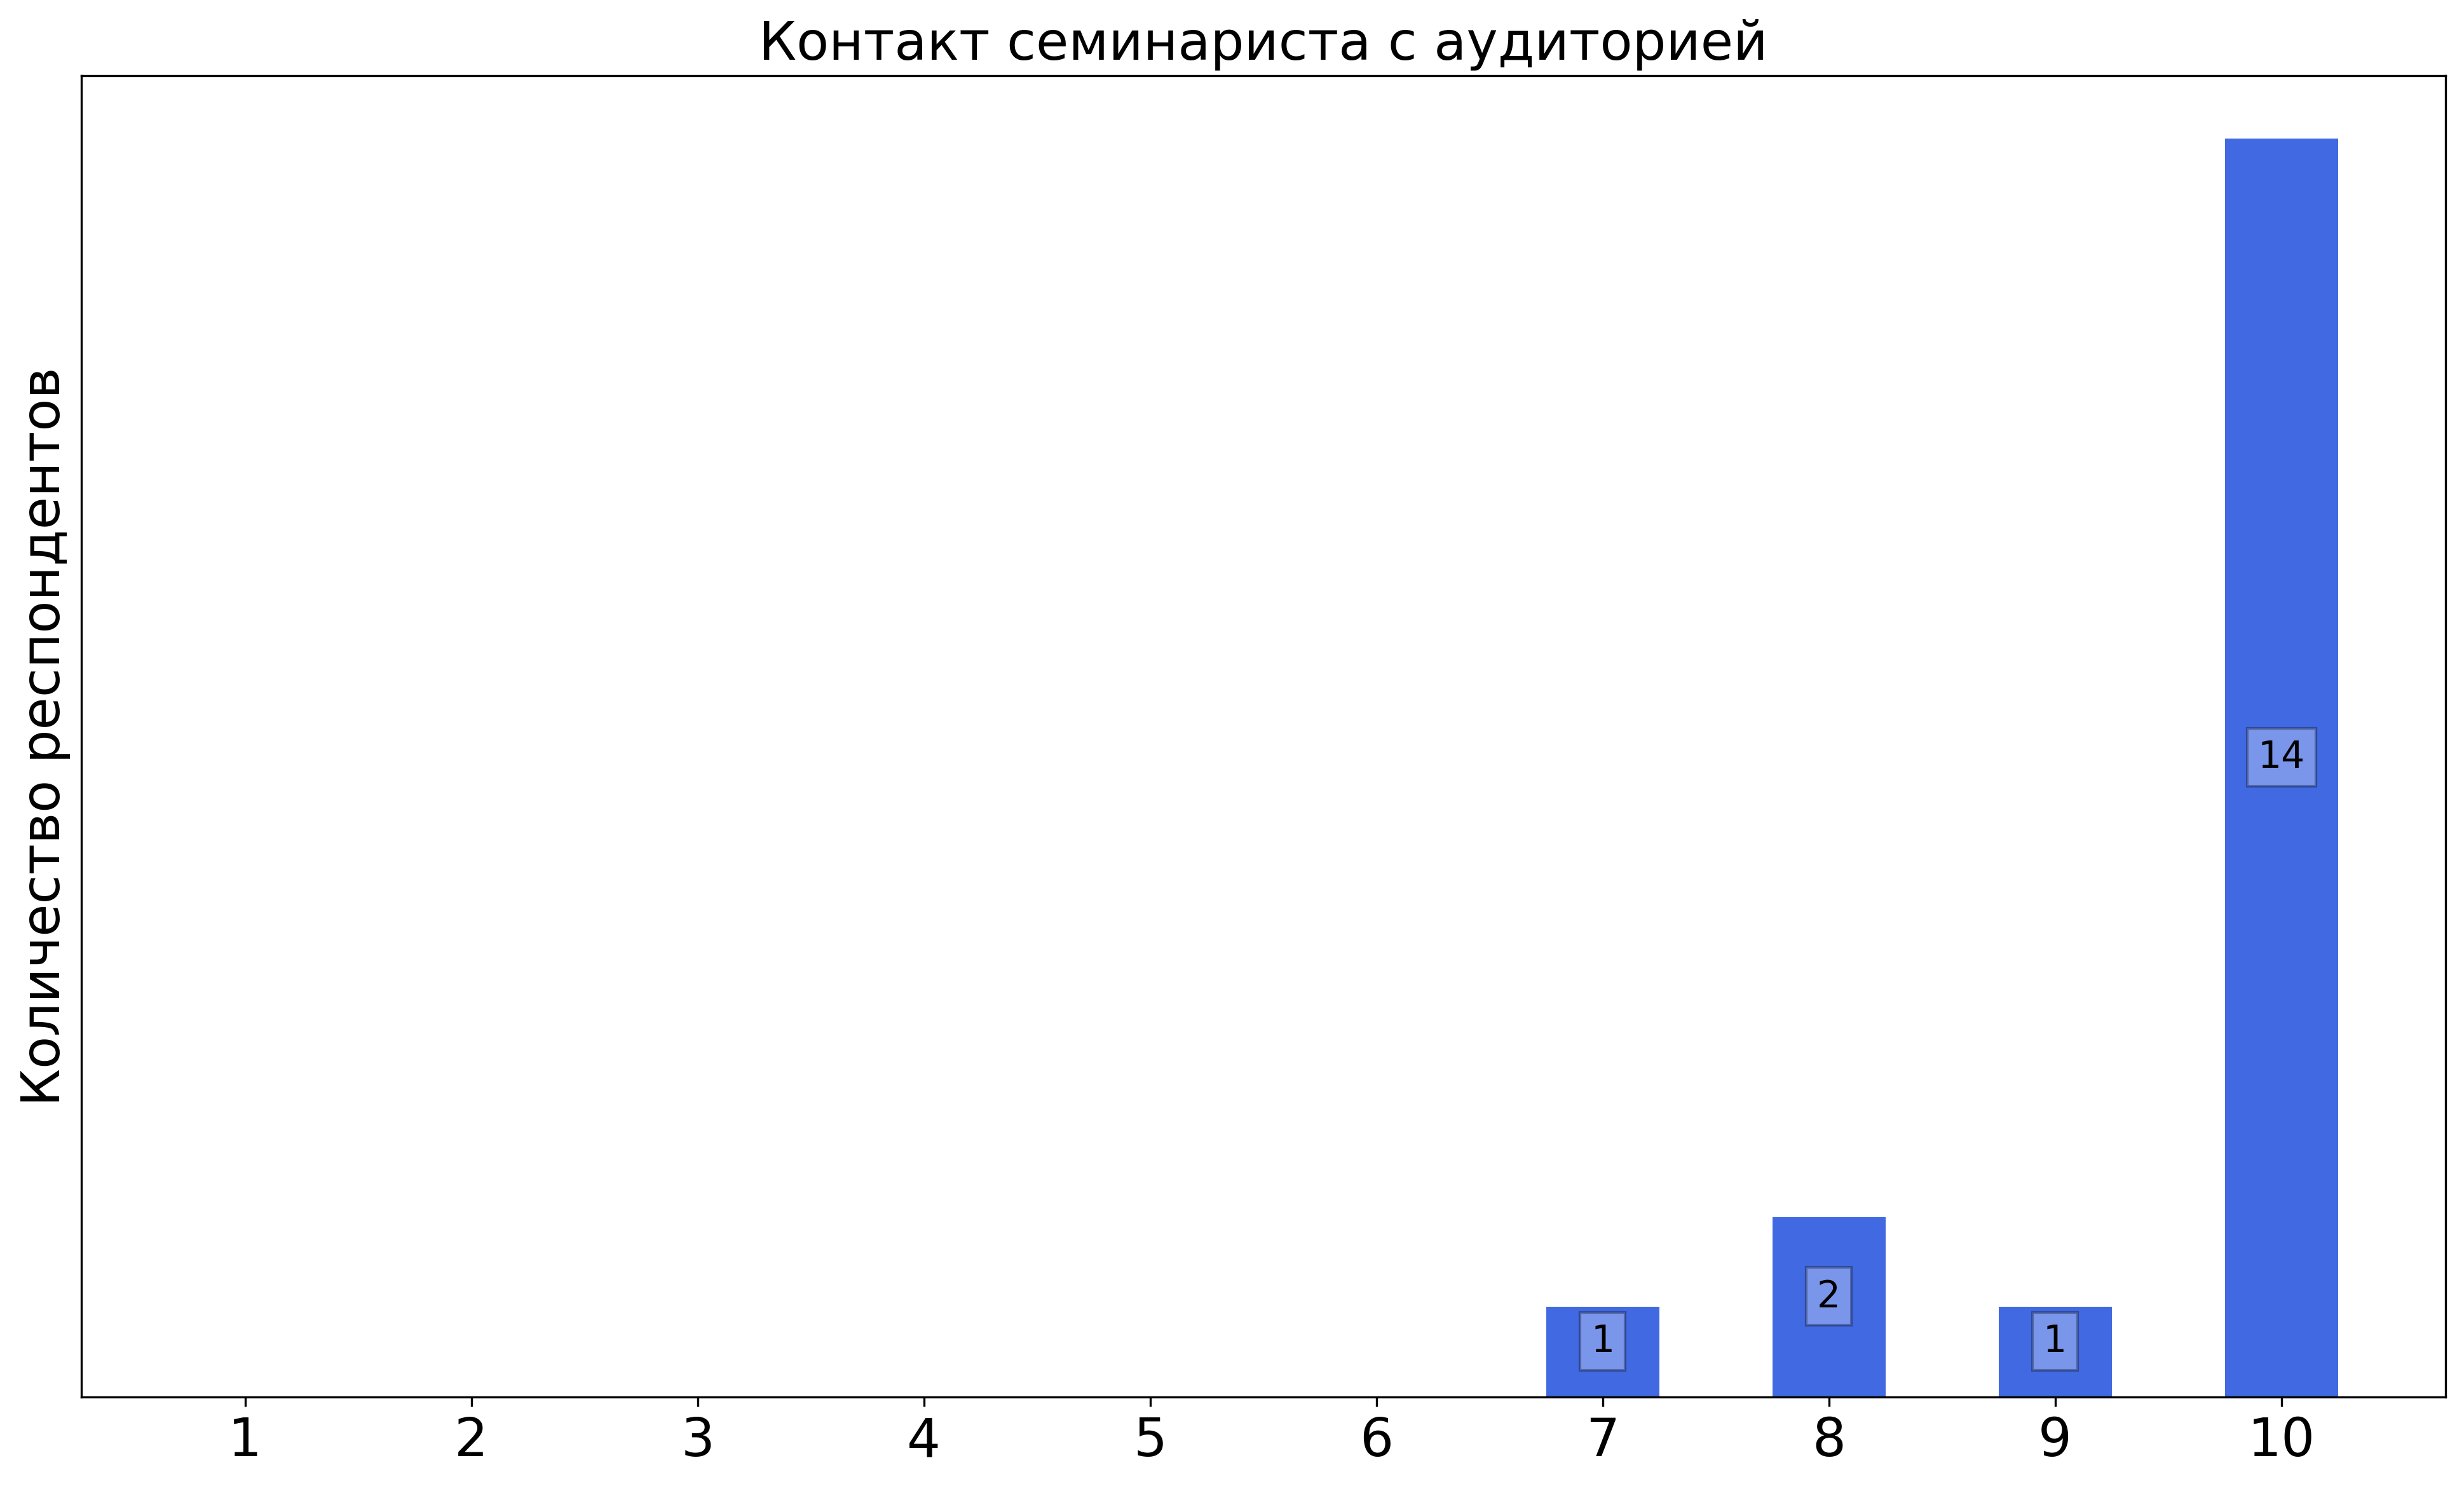
\includegraphics[width=\textwidth]{images/3 course/Вычислительная математика/seminarists-marks-Кожемяченко А.А.-0.png}
			\end{subfigure}
			\begin{subfigure}[b]{0.45\textwidth}
				\centering
				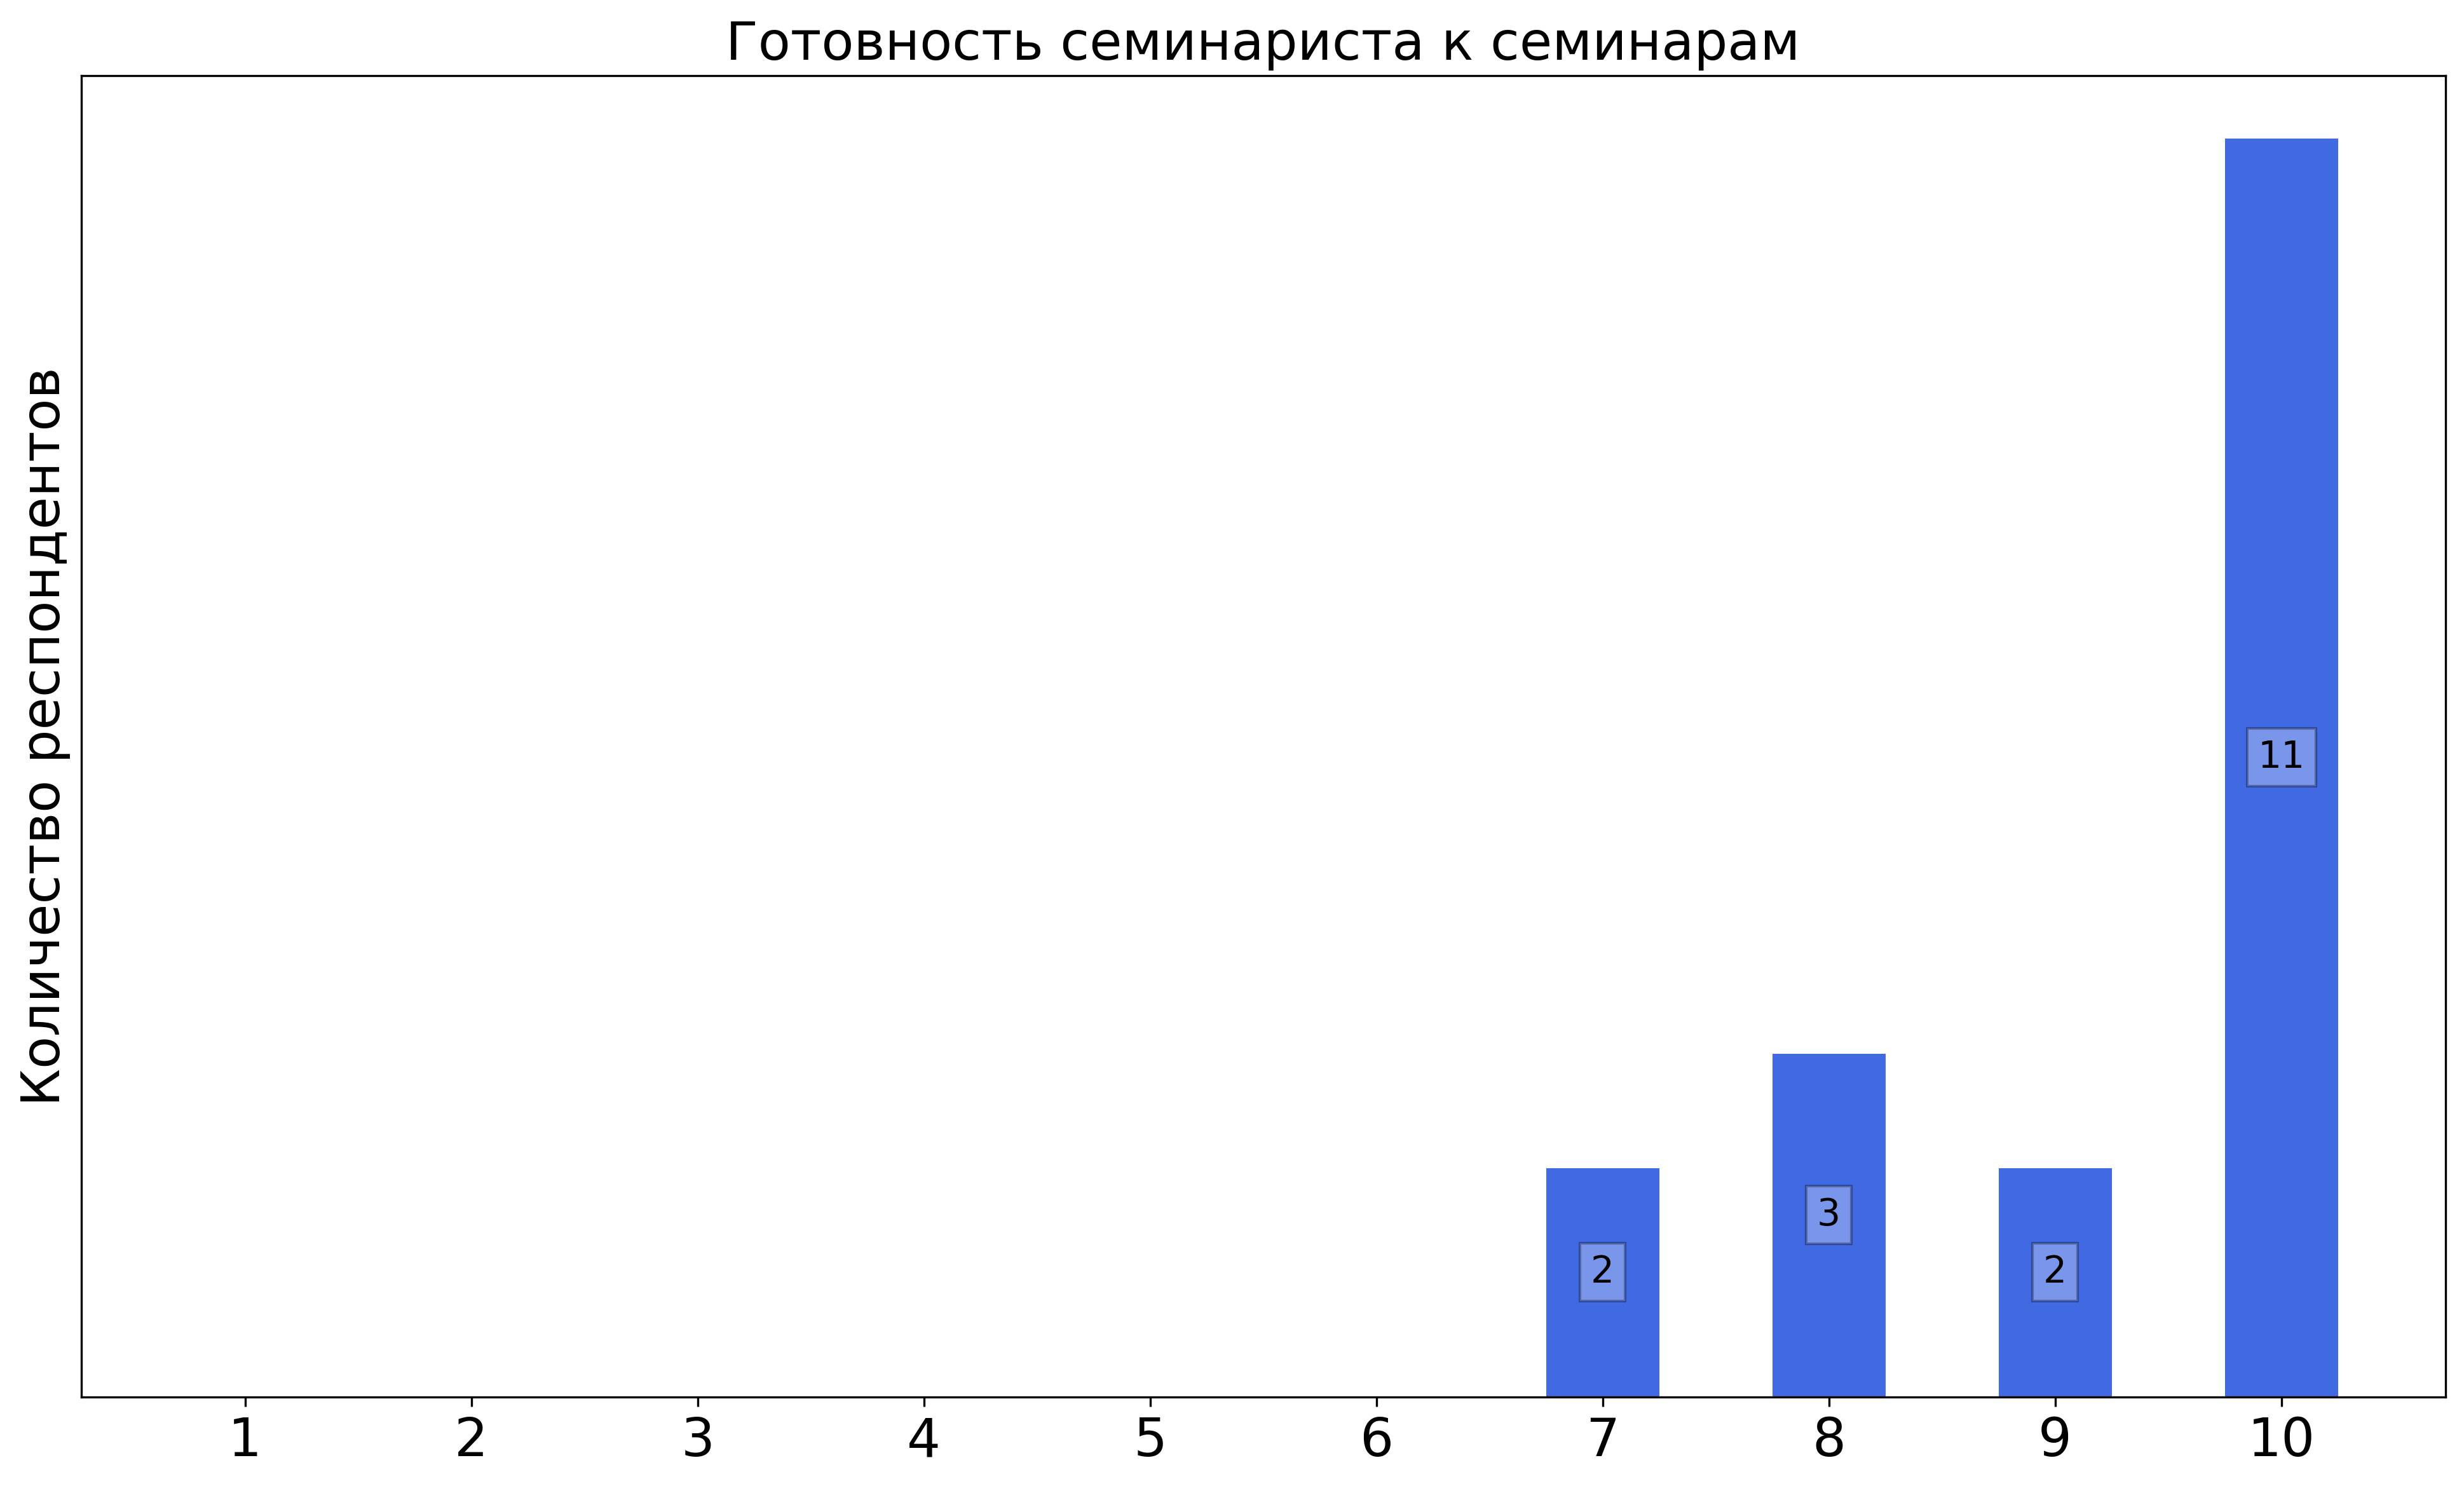
\includegraphics[width=\textwidth]{images/3 course/Вычислительная математика/seminarists-marks-Кожемяченко А.А.-1.png}
			\end{subfigure}
			\begin{subfigure}[b]{0.45\textwidth}
				\centering
				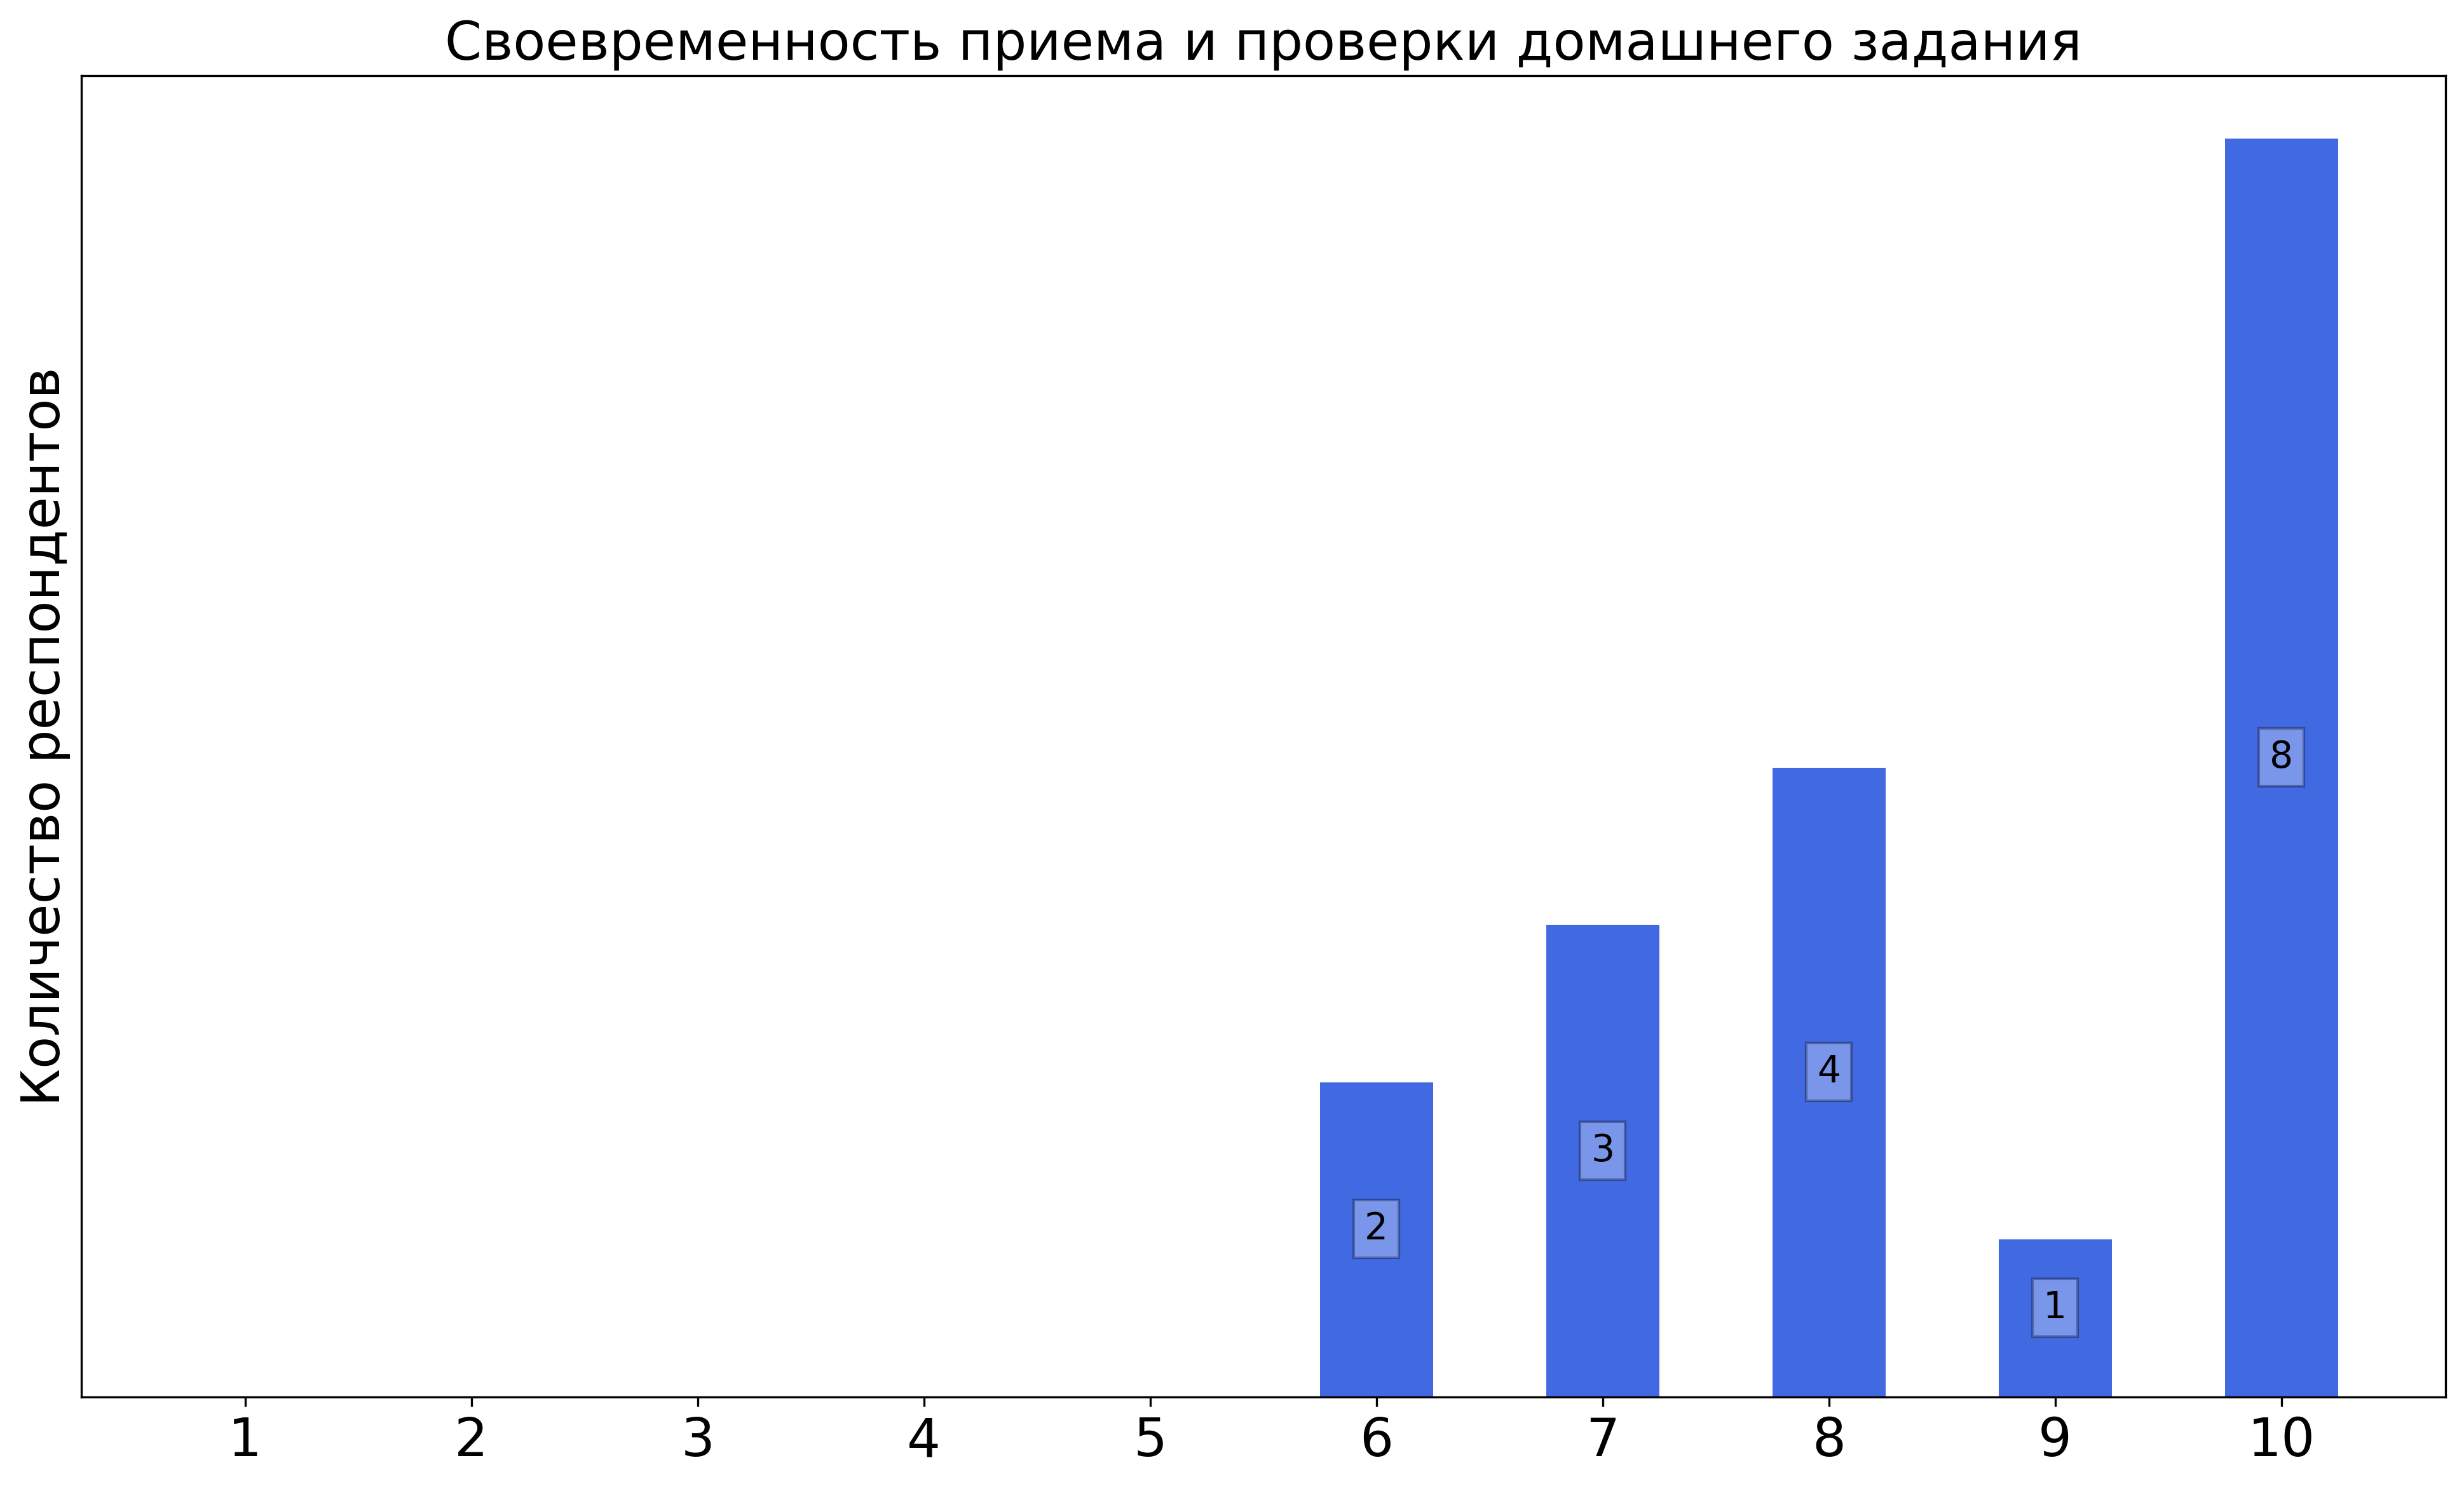
\includegraphics[width=\textwidth]{images/3 course/Вычислительная математика/seminarists-marks-Кожемяченко А.А.-2.png}
			\end{subfigure}
			\begin{subfigure}[b]{0.45\textwidth}
				\centering
				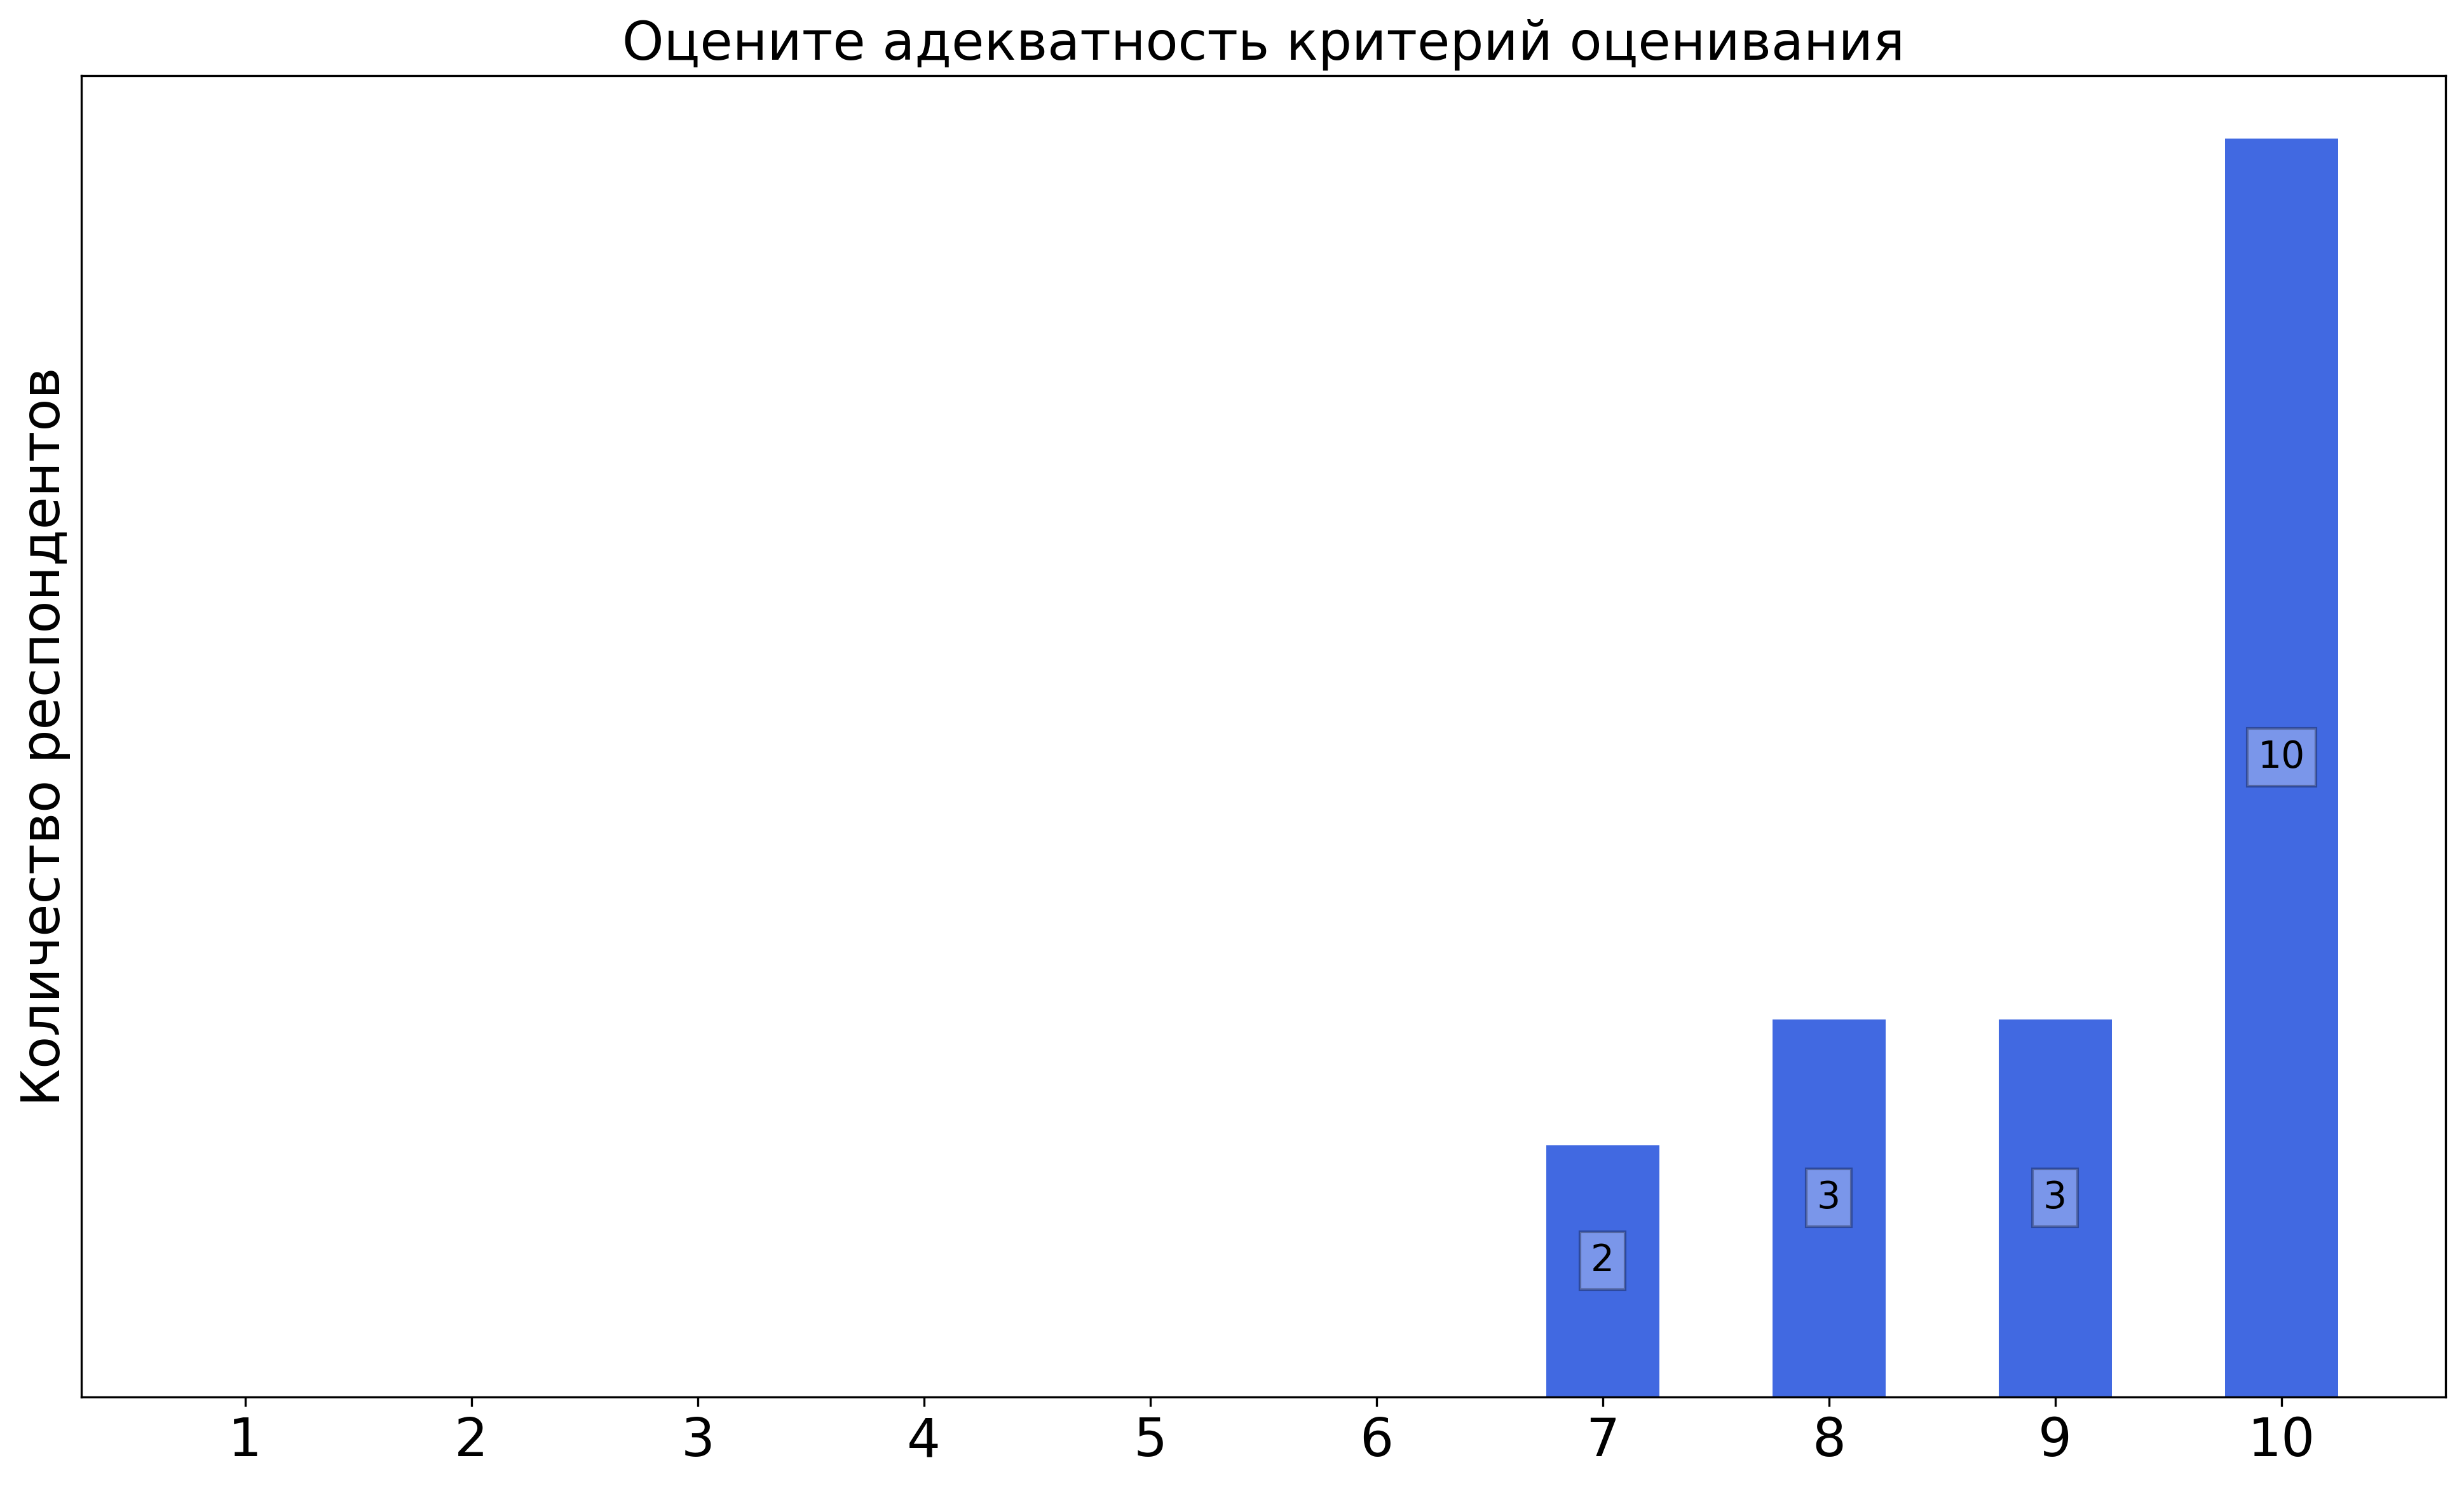
\includegraphics[width=\textwidth]{images/3 course/Вычислительная математика/seminarists-marks-Кожемяченко А.А.-3.png}
			\end{subfigure}	
			\caption{Оценки респондентов о качестве преподавания семинаров}
		\end{figure}


		\textbf{Комментарии студентов о семинаристе\protect\footnote{сохранены оригинальные орфография и пунктуация}}
            \begin{commentbox} 
                Хорошие семинары, добрый семинарист, старается всё объяснить, приятно ходить на семинары 
            \end{commentbox} 

            \begin{commentbox} 
                Отличные объяснения. 
            \end{commentbox} 
        
            \begin{commentbox} 
                Отличные у семинары: минимум теории и разбор задач, а лабы на дом. На контрольных исключительно задачи (знаю, что у многих была на контрольных теория, что, на мой взгляд, не нужно). 
            \end{commentbox} 
        
            \begin{commentbox} 
                Очень классный препод. Мне предмет вообще не интересен, но на семинары я ходил только из-за него 
            \end{commentbox} 
        
            \begin{commentbox} 
                Хорошие семинары, с точки зрения практических приложений методов вычислительной математики всё понятно, чётко. Лабы прекрасные! Когда сам что-то делаешь - лучше разбираешься. Также нам скидывают все методички где можно дополнительно прочесть материалы с семинаров 
            \end{commentbox} 
        
            \begin{commentbox} 
                Больше было именно практических знаний и лабораторных работ, что позволило лучше осознать полезность данного предмета. Теоретические упражнения также были, однако им роль отводилась больше для примеров и контрольных работ, которые можно было спокойно написать на высокий балл, если посещал семинары. 
            \end{commentbox} 
        
            \begin{commentbox} 
                Рассказывает хорошо, лабы принимает халявно. Контрольные нормальные  
            \end{commentbox} 
        
            \begin{commentbox} 
                Замечательный семинарист, всегда очень интересно и доступно излагает материал и ответственно готовится к семинарам. Антон Андреевич использует в учебном процессе большое число источников не из списка литературы, которые помогают в освоении курса. Семинаров и рекомендуемой семинаристом литературы полностью хватает для выполнения лабораторных работ и написания контрольных, на семинары хожу с удовольствием. 
            \end{commentbox} 
        
            \begin{commentbox} 
                Очень хорош. Разбирает на семинарах то, что потом окажется в контрольной. Понятно и четко выдает материал. Очень приятный как преподаватель и как собеседник 
            \end{commentbox}


    \subsubsection{Отзыв студентов о семинарах. Семинарист: Конев С.А.}
        \begin{figure}[H]
            \centering
            \begin{subfigure}[b]{0.45\textwidth}
                \centering
                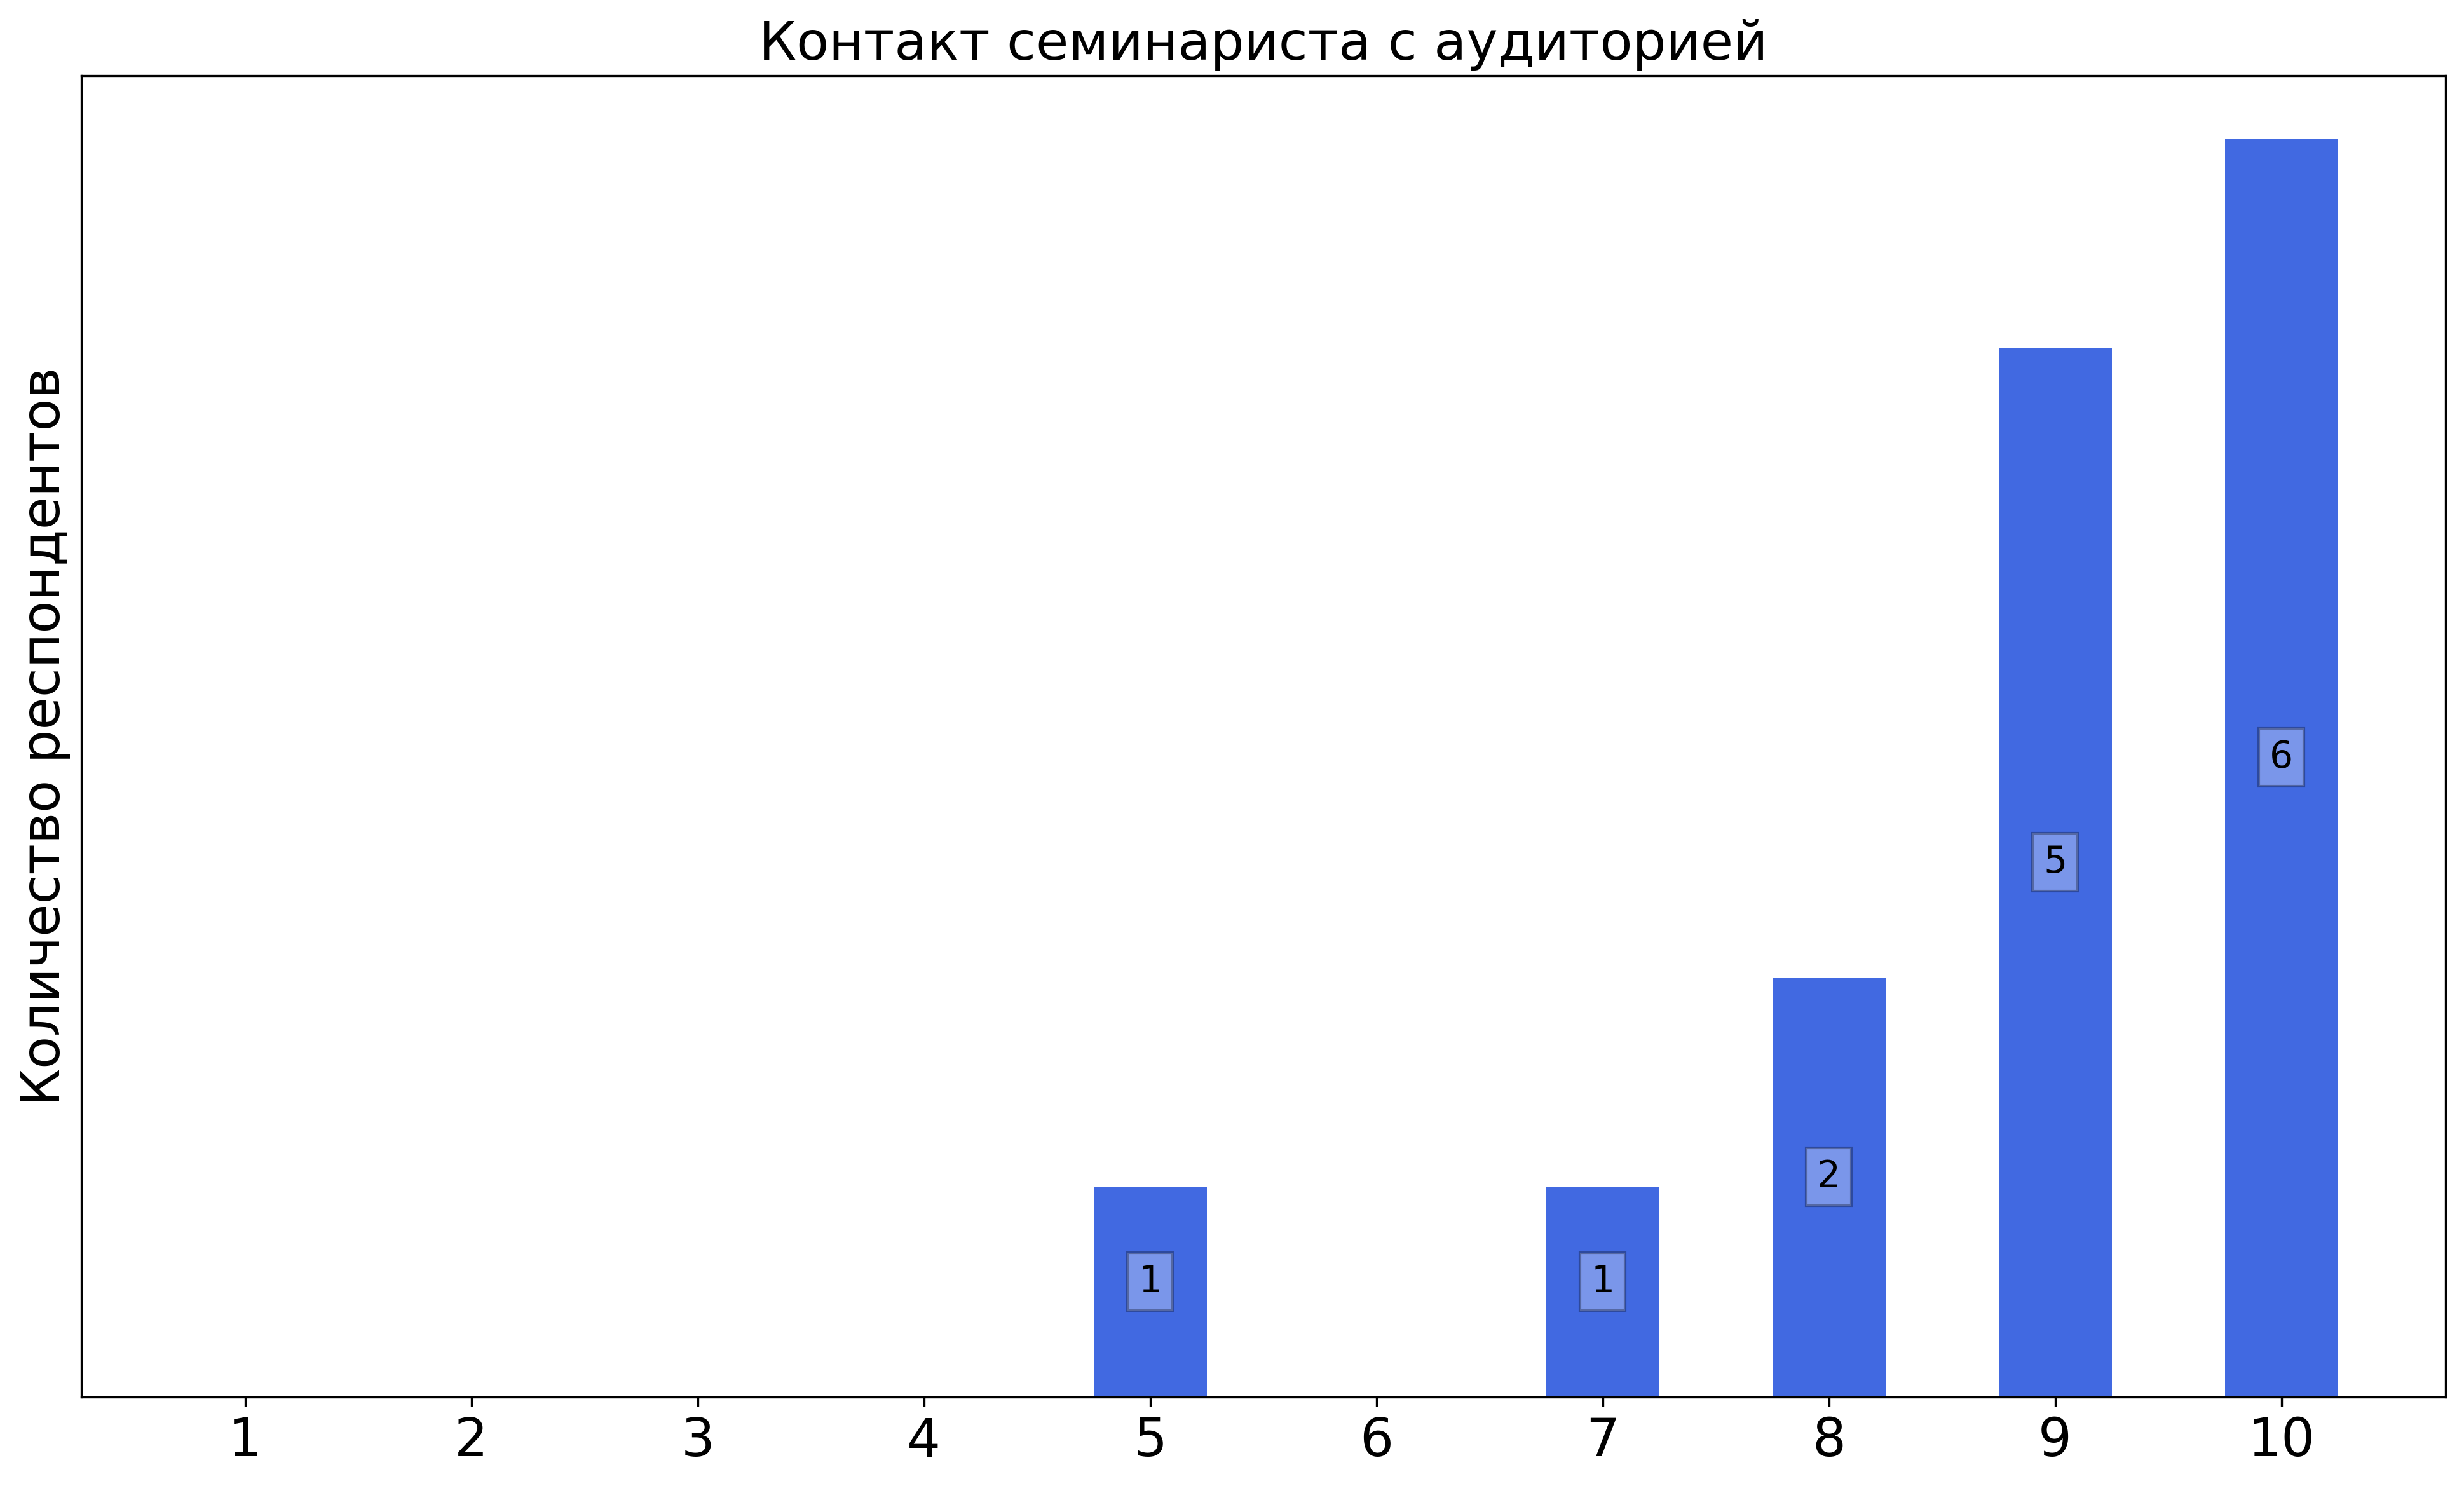
\includegraphics[width=\textwidth]{images/3 course/Вычислительная математика/seminarists-marks-Конев С.А.-0.png}
            \end{subfigure}
            \begin{subfigure}[b]{0.45\textwidth}
                \centering
                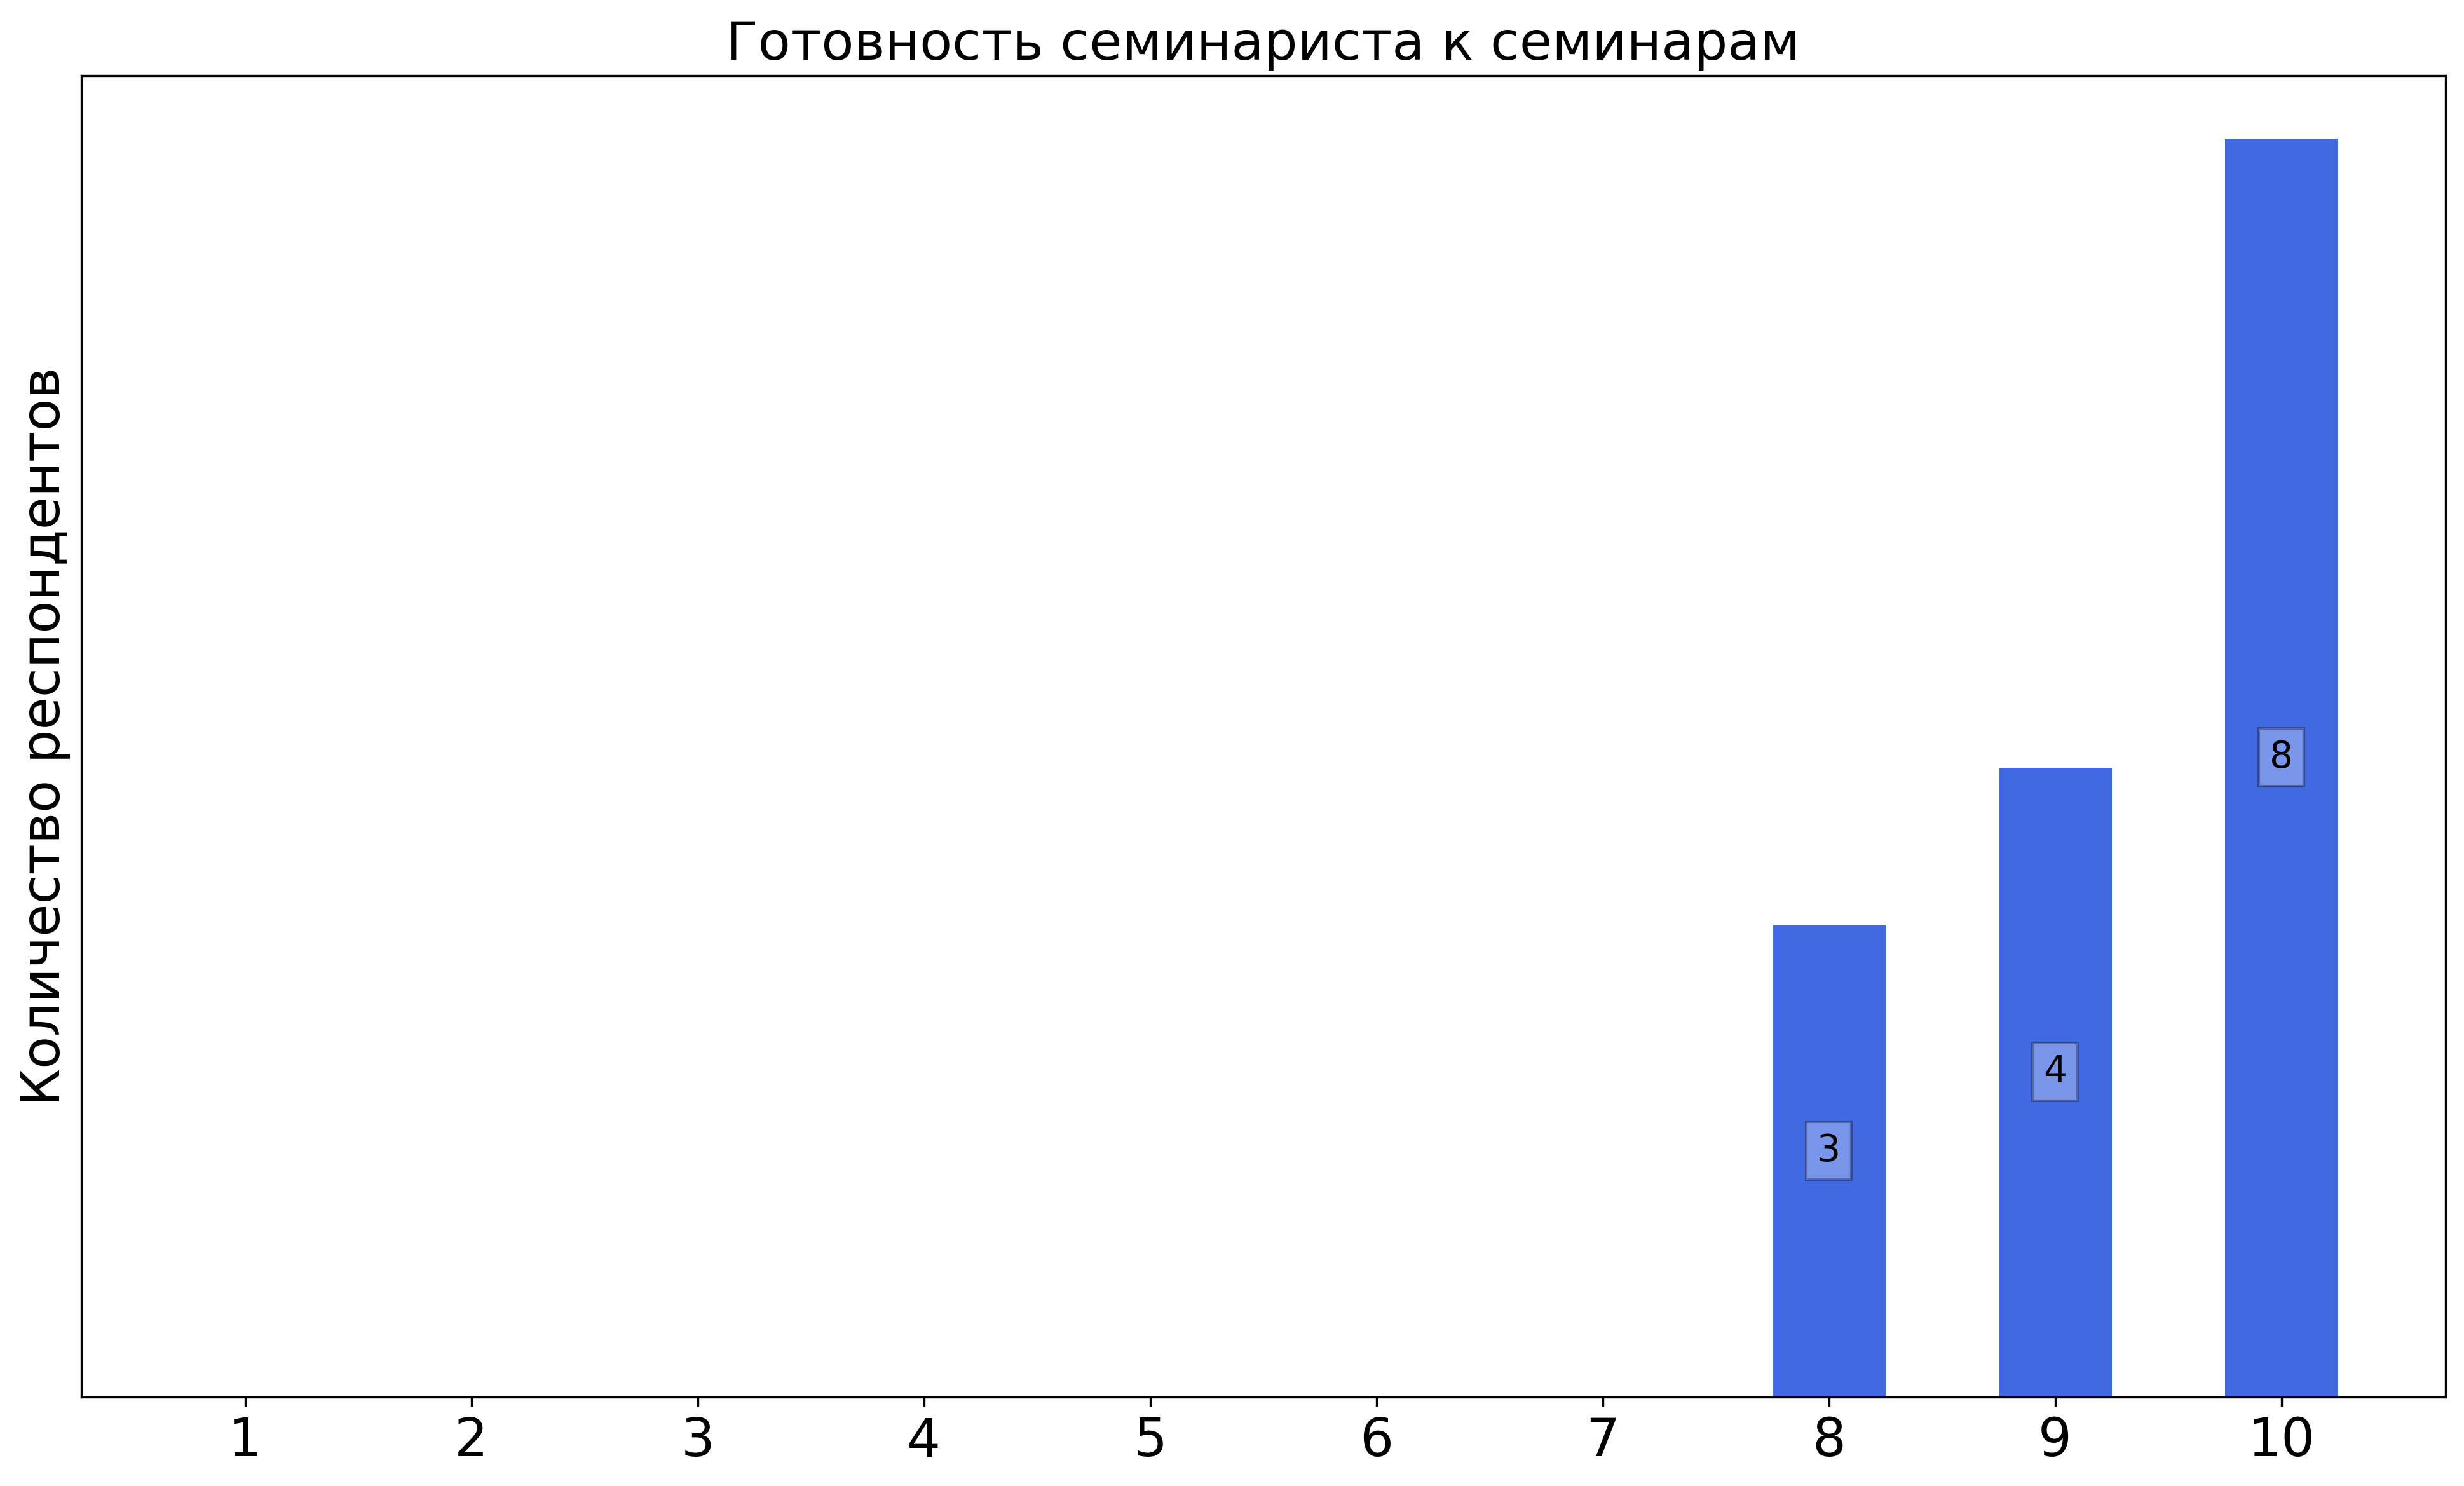
\includegraphics[width=\textwidth]{images/3 course/Вычислительная математика/seminarists-marks-Конев С.А.-1.png}
            \end{subfigure}
            \begin{subfigure}[b]{0.45\textwidth}
                \centering
                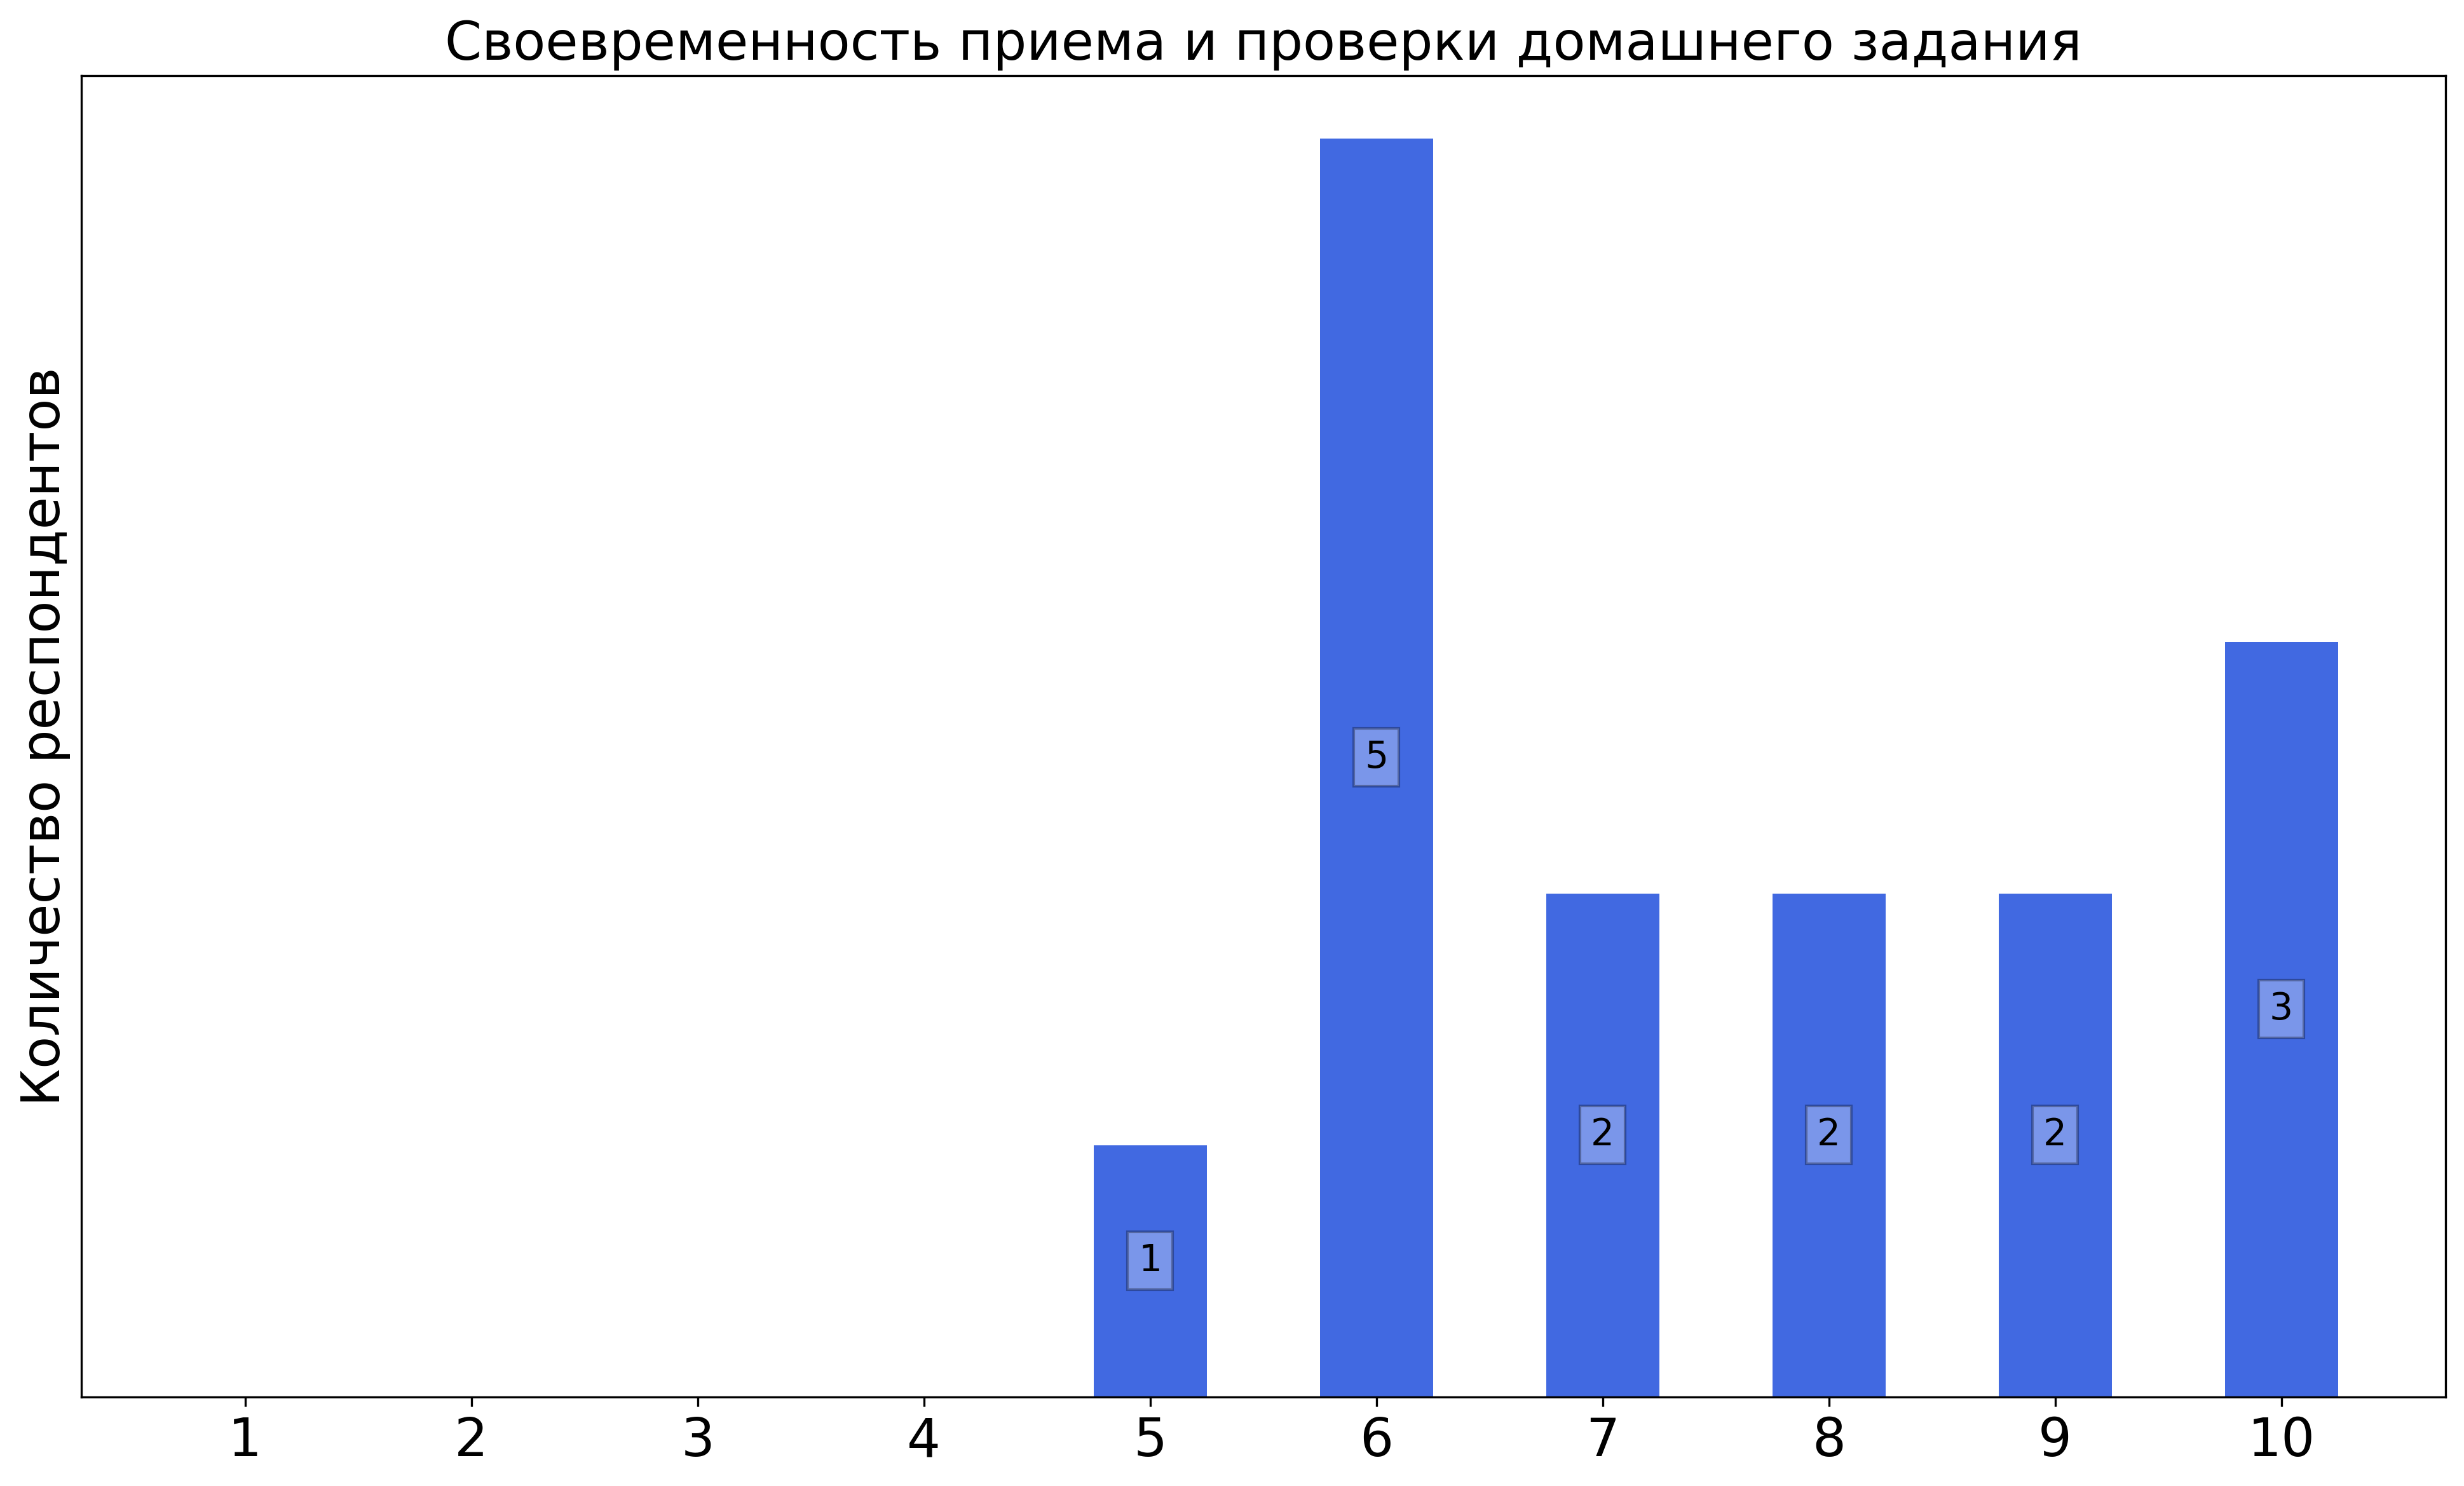
\includegraphics[width=\textwidth]{images/3 course/Вычислительная математика/seminarists-marks-Конев С.А.-2.png}
            \end{subfigure}
            \begin{subfigure}[b]{0.45\textwidth}
                \centering
                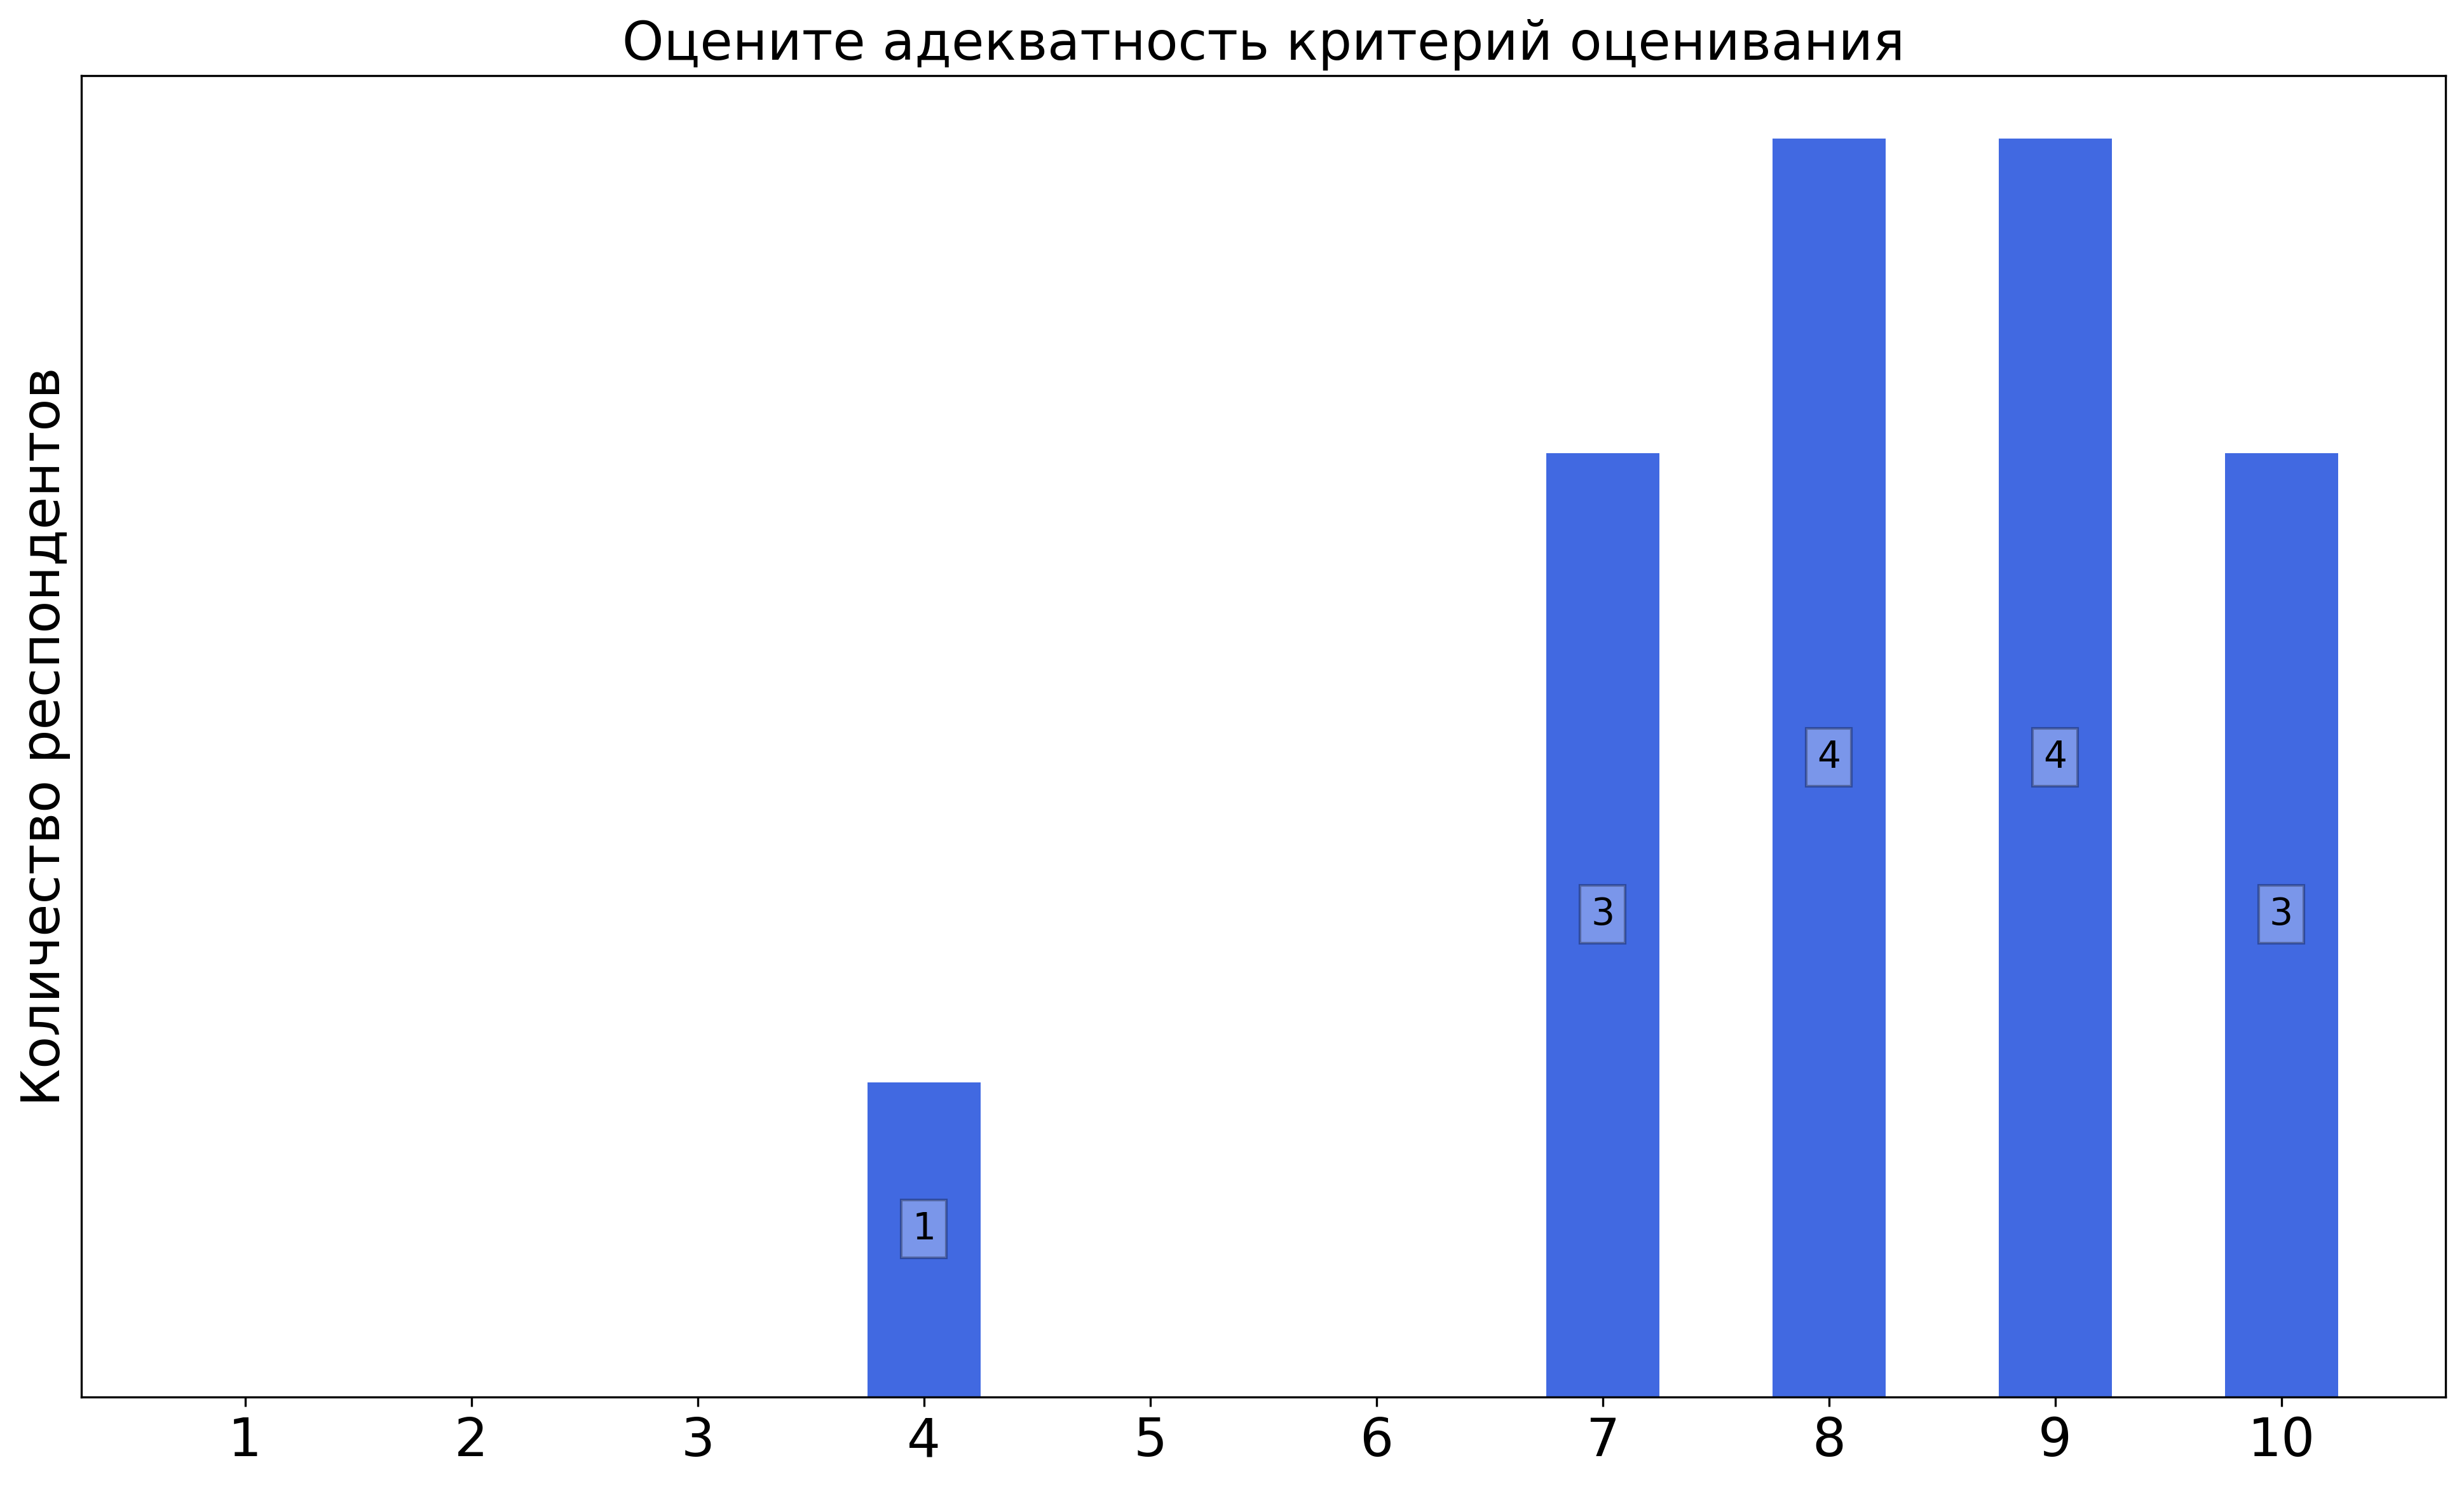
\includegraphics[width=\textwidth]{images/3 course/Вычислительная математика/seminarists-marks-Конев С.А.-3.png}
            \end{subfigure}	
            \caption{Оценки респондентов о качестве преподавания семинаров}
        \end{figure}

        \textbf{Комментарии студентов о семинаристе\protect\footnote{сохранены оригинальные орфография и пунктуация}}
            \begin{commentbox} 
                Достаточно молодой, хорошо преподает, заинтересован в предмете, но только первый год на физтехе, это чувсвуется 
            \end{commentbox} 

            \begin{commentbox} 
                Действительно крутой преподаватель, но без нормальных лекций крайне сложно что-то воспринимать. Контрольные необъективно сложно 
            \end{commentbox} 

            \begin{commentbox} 
                Мне понравились семинары Конева С.А. Хоть он и недавно на физтехе, но с программой был хорошо знаком. Любит свой предмет, часто приводит примеры, где может пригодиться проходимая тема. У него были довольно трудные контрольные, но по итогу оценки вышли у всех справедливые. Идёт навстречу, если нужно устроить доп семинар. Я рекомендовал бы его другим студентам. 
            \end{commentbox} 

            \begin{commentbox} 
                Молодой преподаватель, система ещё не до конца выстроена - в течение семестра менялись критерии оценивания, контрольные невозможно решить за 1 пару. Несмотря на небольшой опыт, материал излагает интересно и доступно, приятный в общении 
            \end{commentbox} 

            \begin{commentbox} 
                Семинары отличные, семинарист замечательный, излагаемый материал был структурирован и понятен и позволял при должной концентрации, отсутствии пропусков и осознании решать почти все задачи из программы. К сожалению, семинар проходил первый парой, поэтому не всегда получалось ходить, а когда получалось, концентрации не хватало. Контрольные были сложные, но по делу и с возможностью использования материала и оценивались достаточно лояльно, имели очень конструктивный вклад в изучение предмета. 
            \end{commentbox} 

            \begin{commentbox} 
                Не было уделено времени программированию, на семинарах решали задачи на доске и было много теории. Подробно, из-за чего сильно не успели несколько тем, запланированных в семестре. 
            \end{commentbox} 

            \begin{commentbox} 
                Хорошо объясняет материал. Размытые/переусложнённые критерии оценивания. 
            \end{commentbox} 
        

    \subsubsection{Отзыв студентов о семинарах. Семинарист: Петров М.Н.}
		\begin{figure}[H]
			\centering
			\begin{subfigure}[b]{0.45\textwidth}
				\centering
				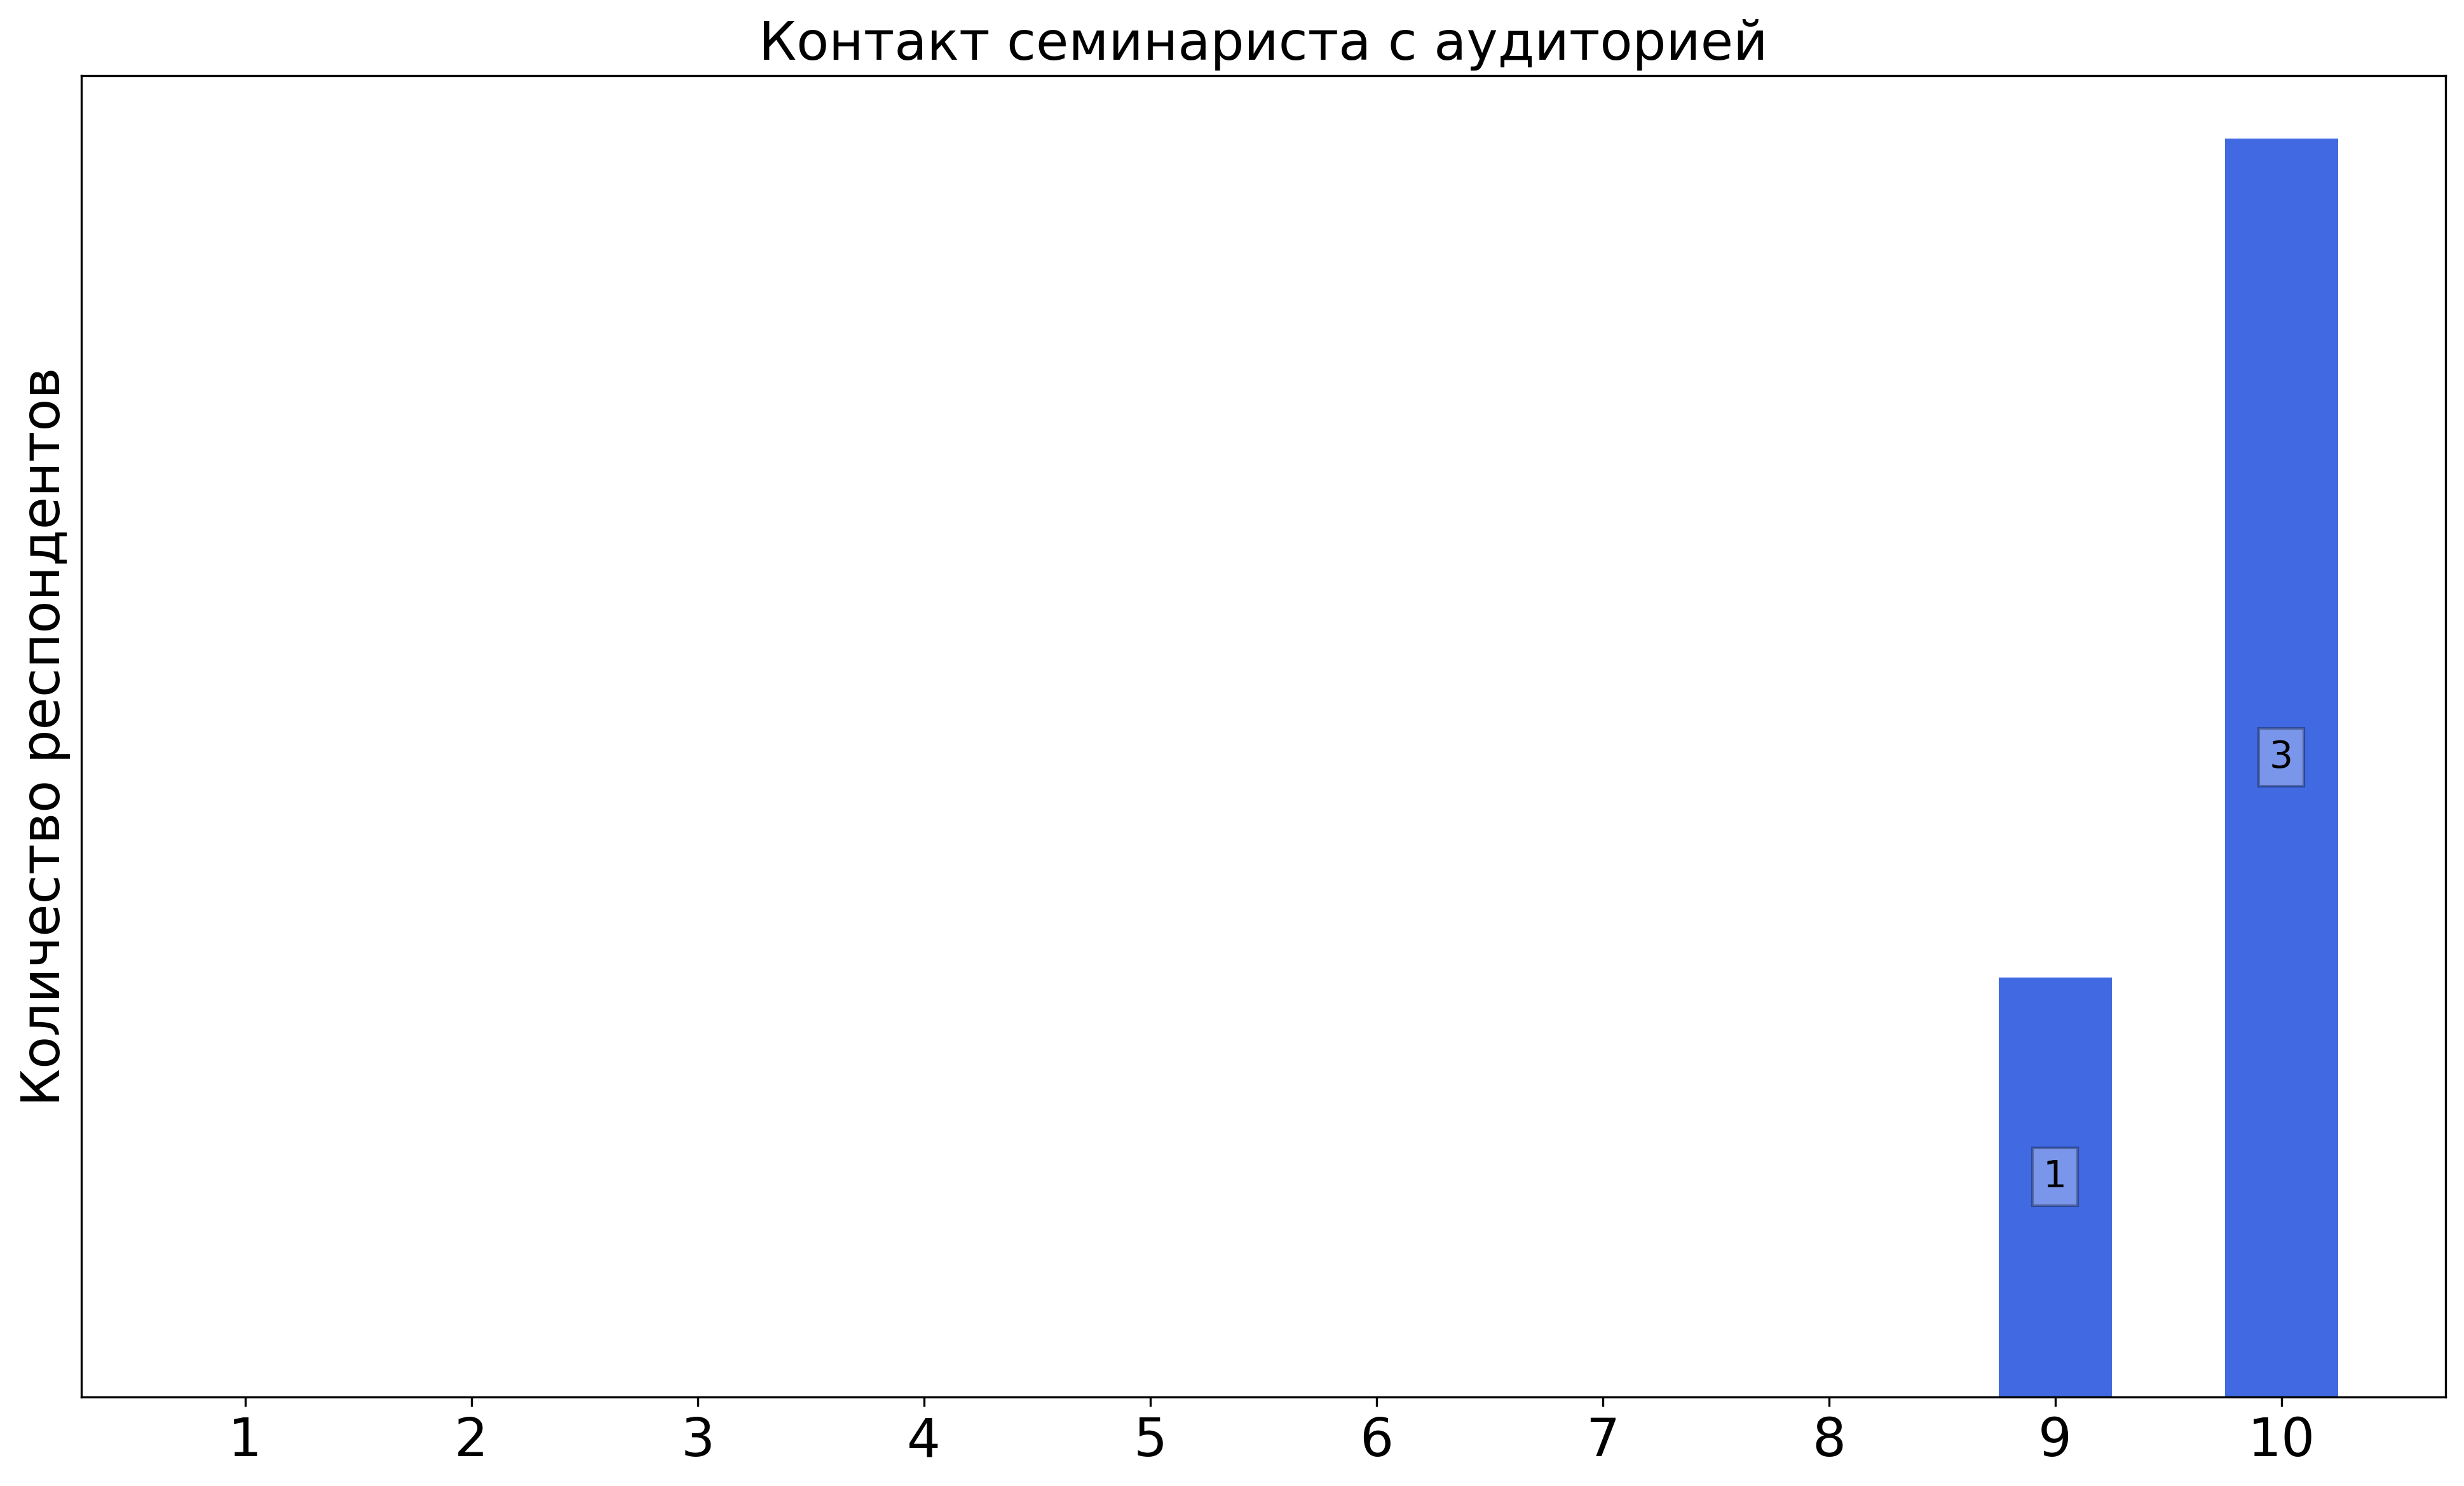
\includegraphics[width=\textwidth]{images/3 course/Вычислительная математика/seminarists-marks-Петров М.Н.-0.png}
			\end{subfigure}
			\begin{subfigure}[b]{0.45\textwidth}
				\centering
				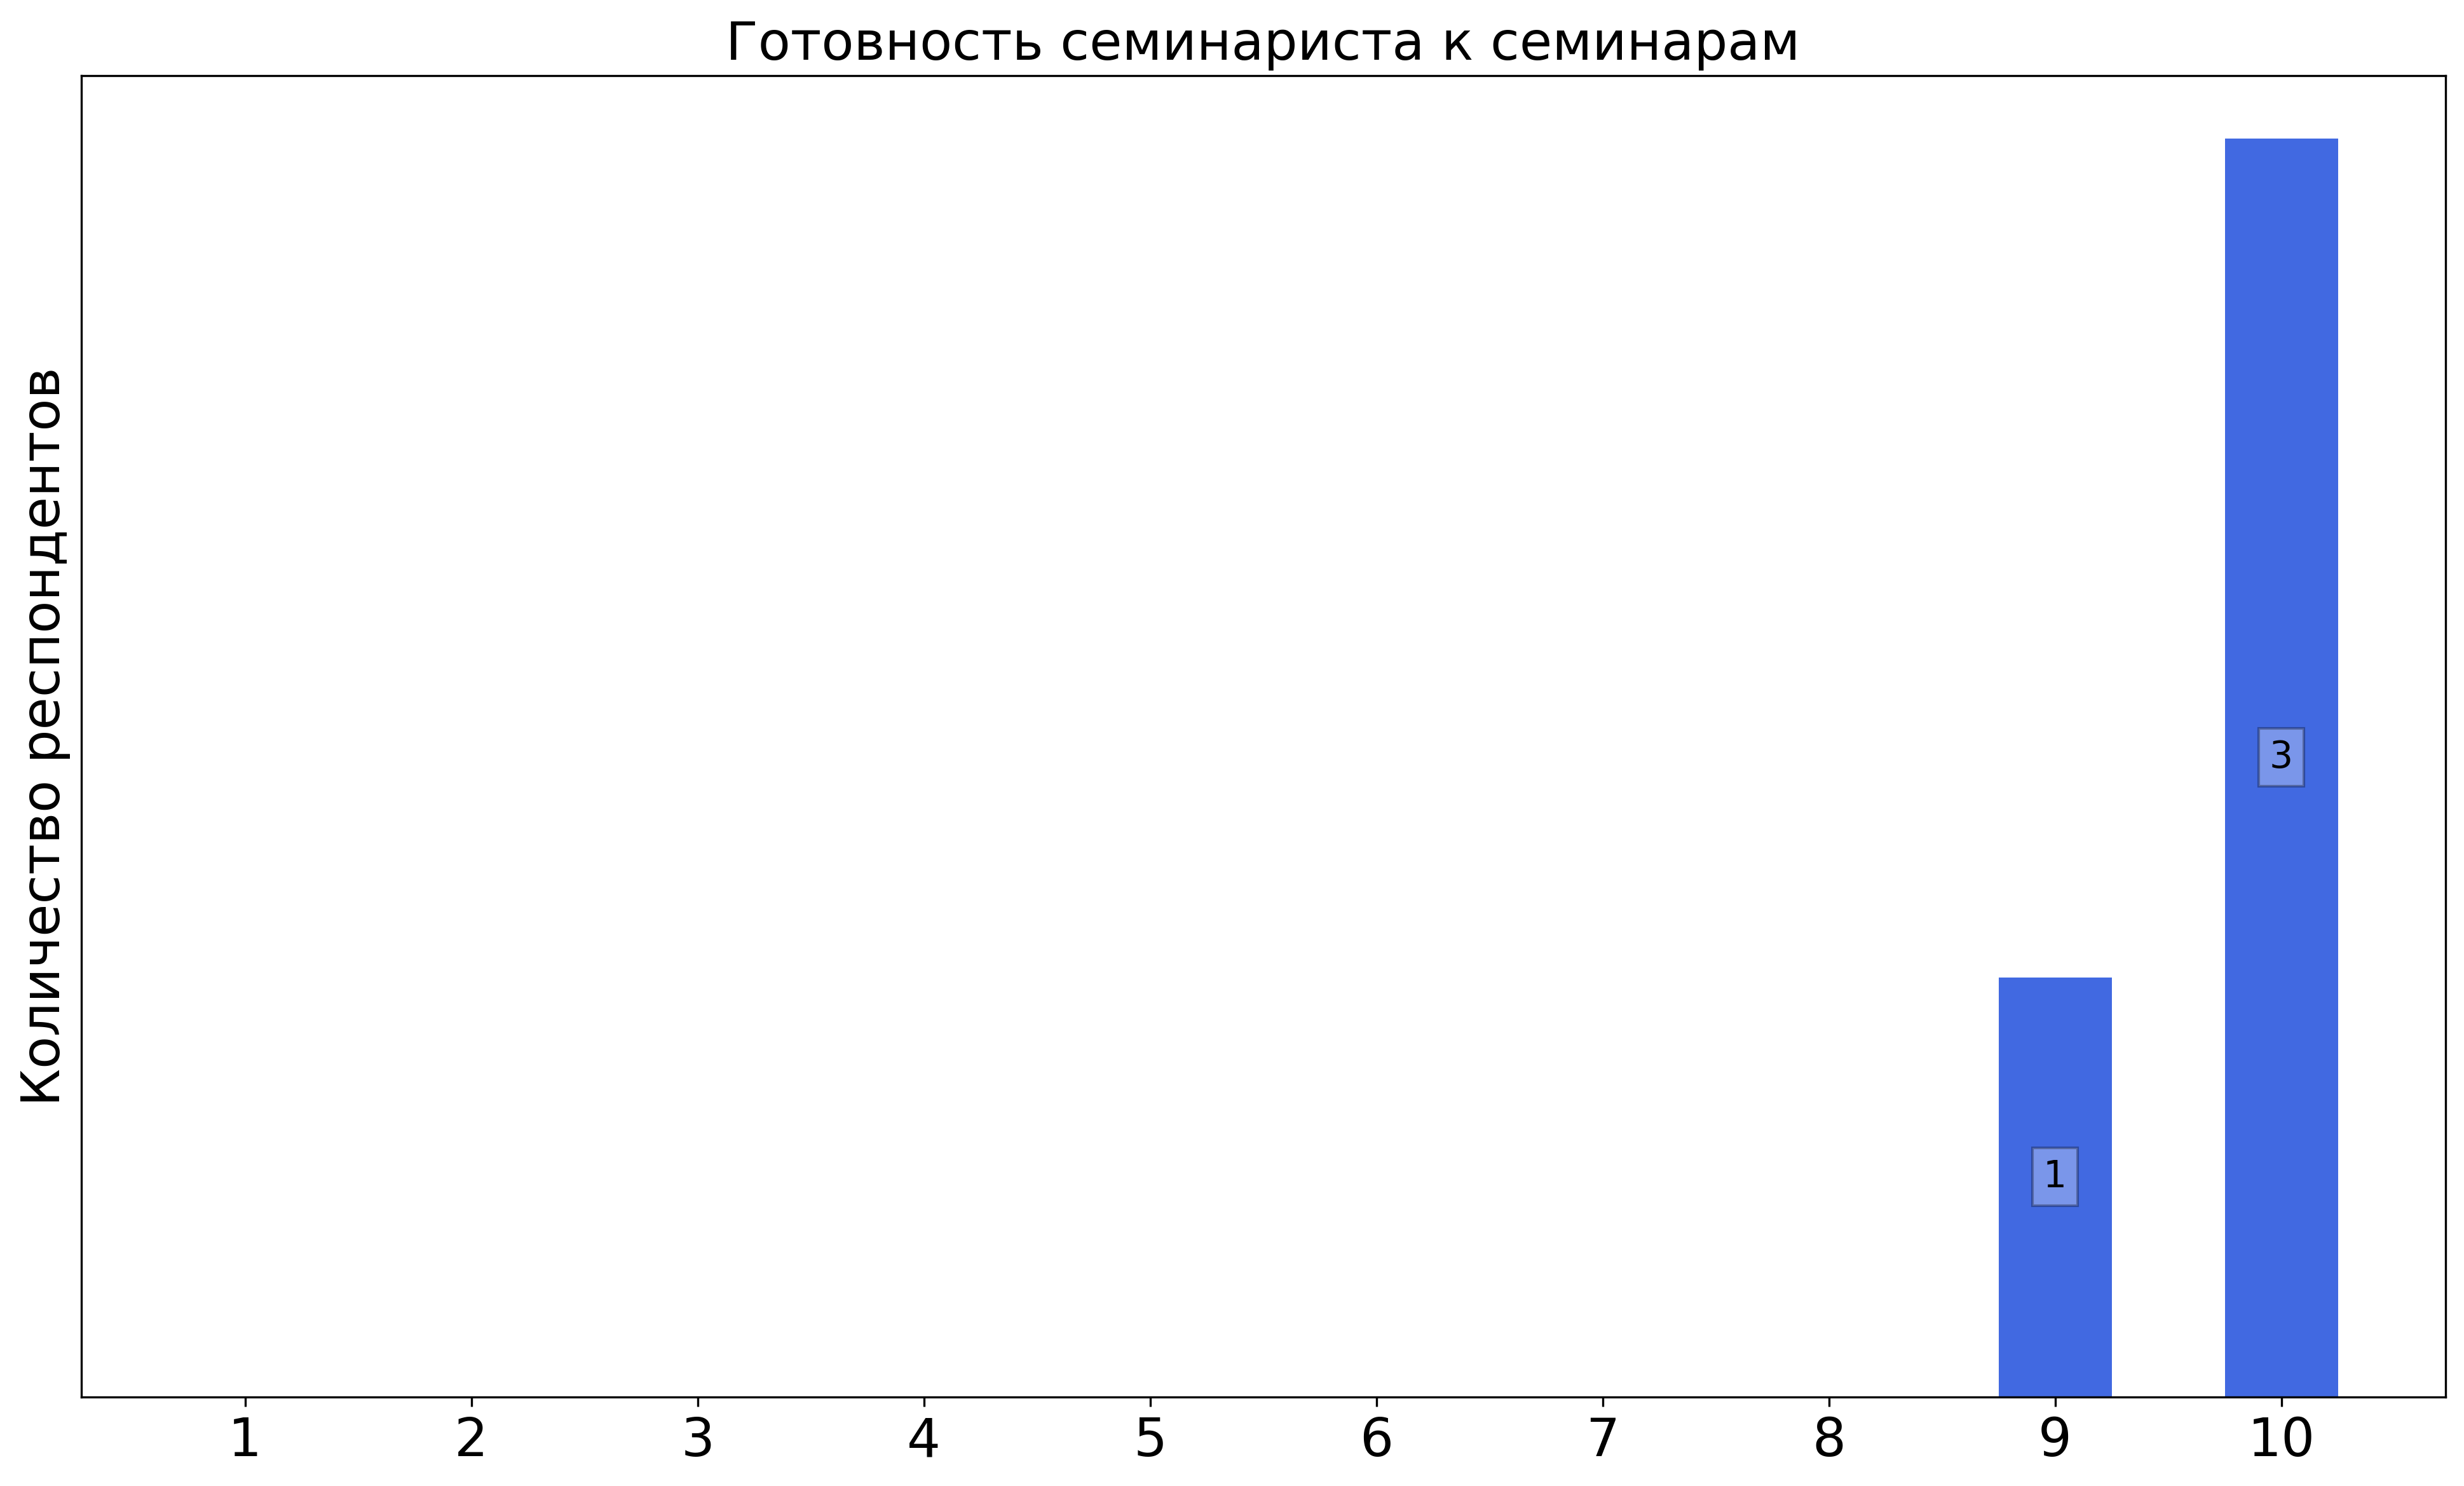
\includegraphics[width=\textwidth]{images/3 course/Вычислительная математика/seminarists-marks-Петров М.Н.-1.png}
			\end{subfigure}
			\begin{subfigure}[b]{0.45\textwidth}
				\centering
				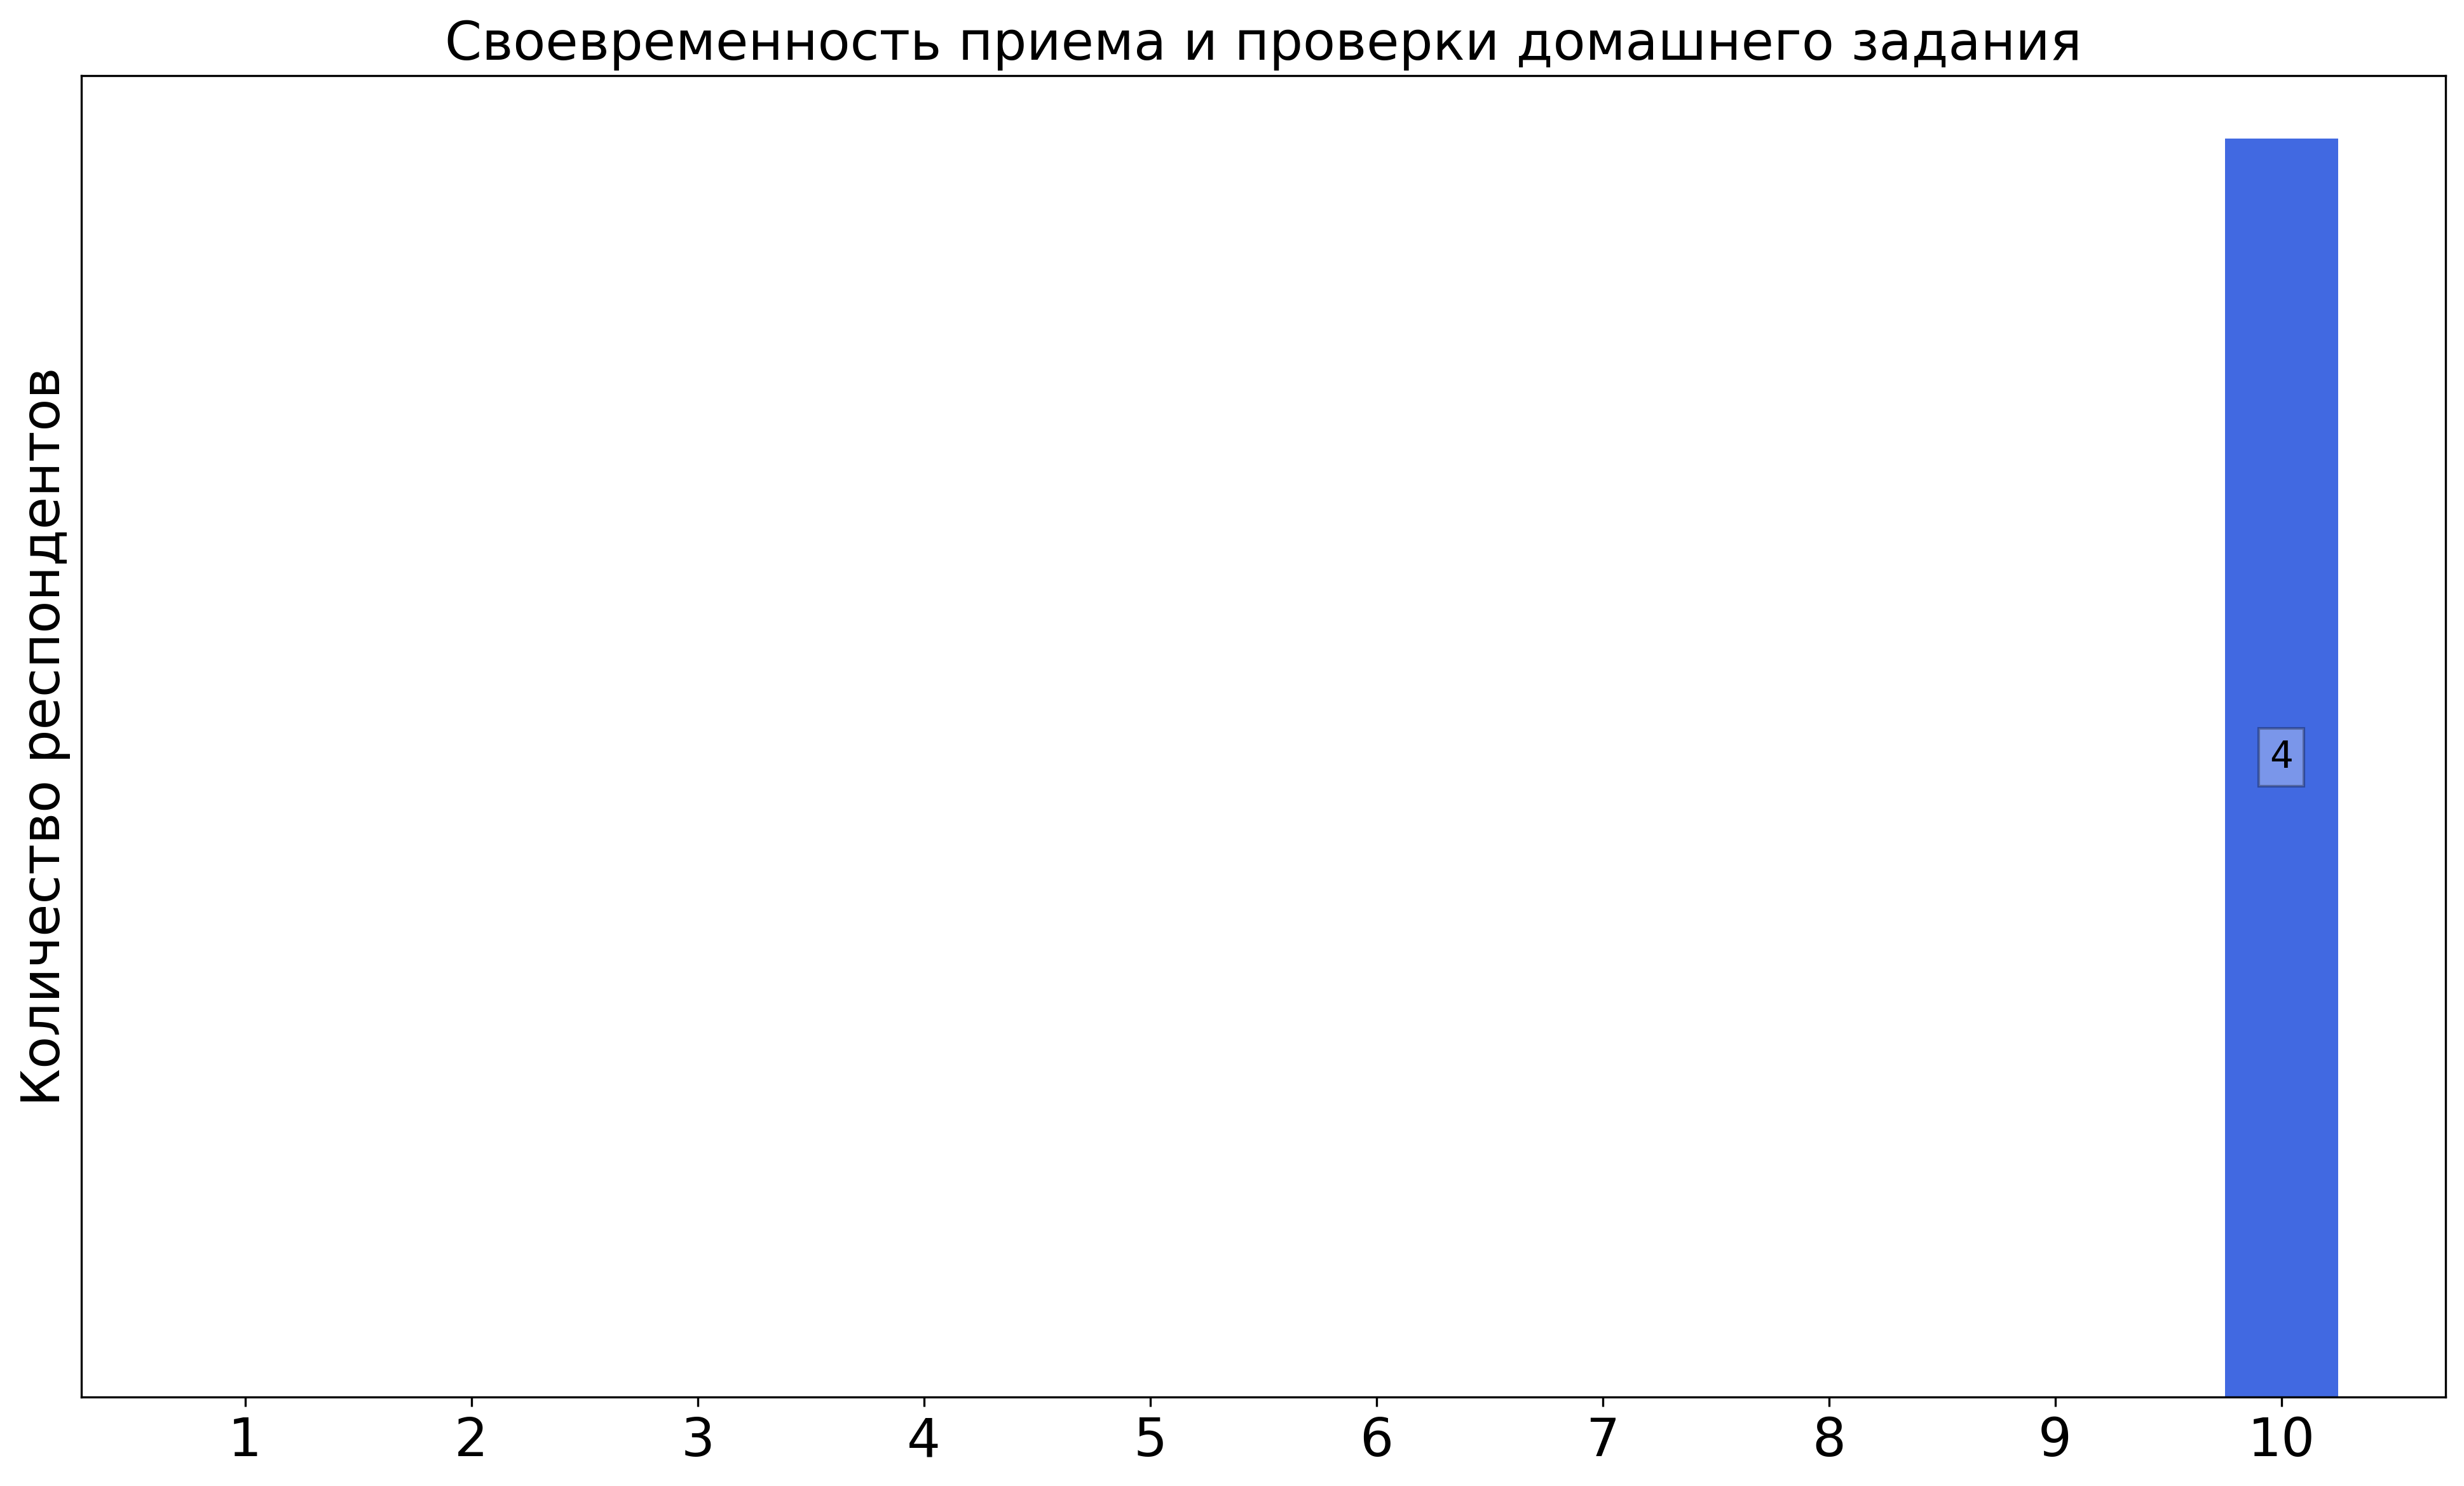
\includegraphics[width=\textwidth]{images/3 course/Вычислительная математика/seminarists-marks-Петров М.Н.-2.png}
			\end{subfigure}
			\begin{subfigure}[b]{0.45\textwidth}
				\centering
				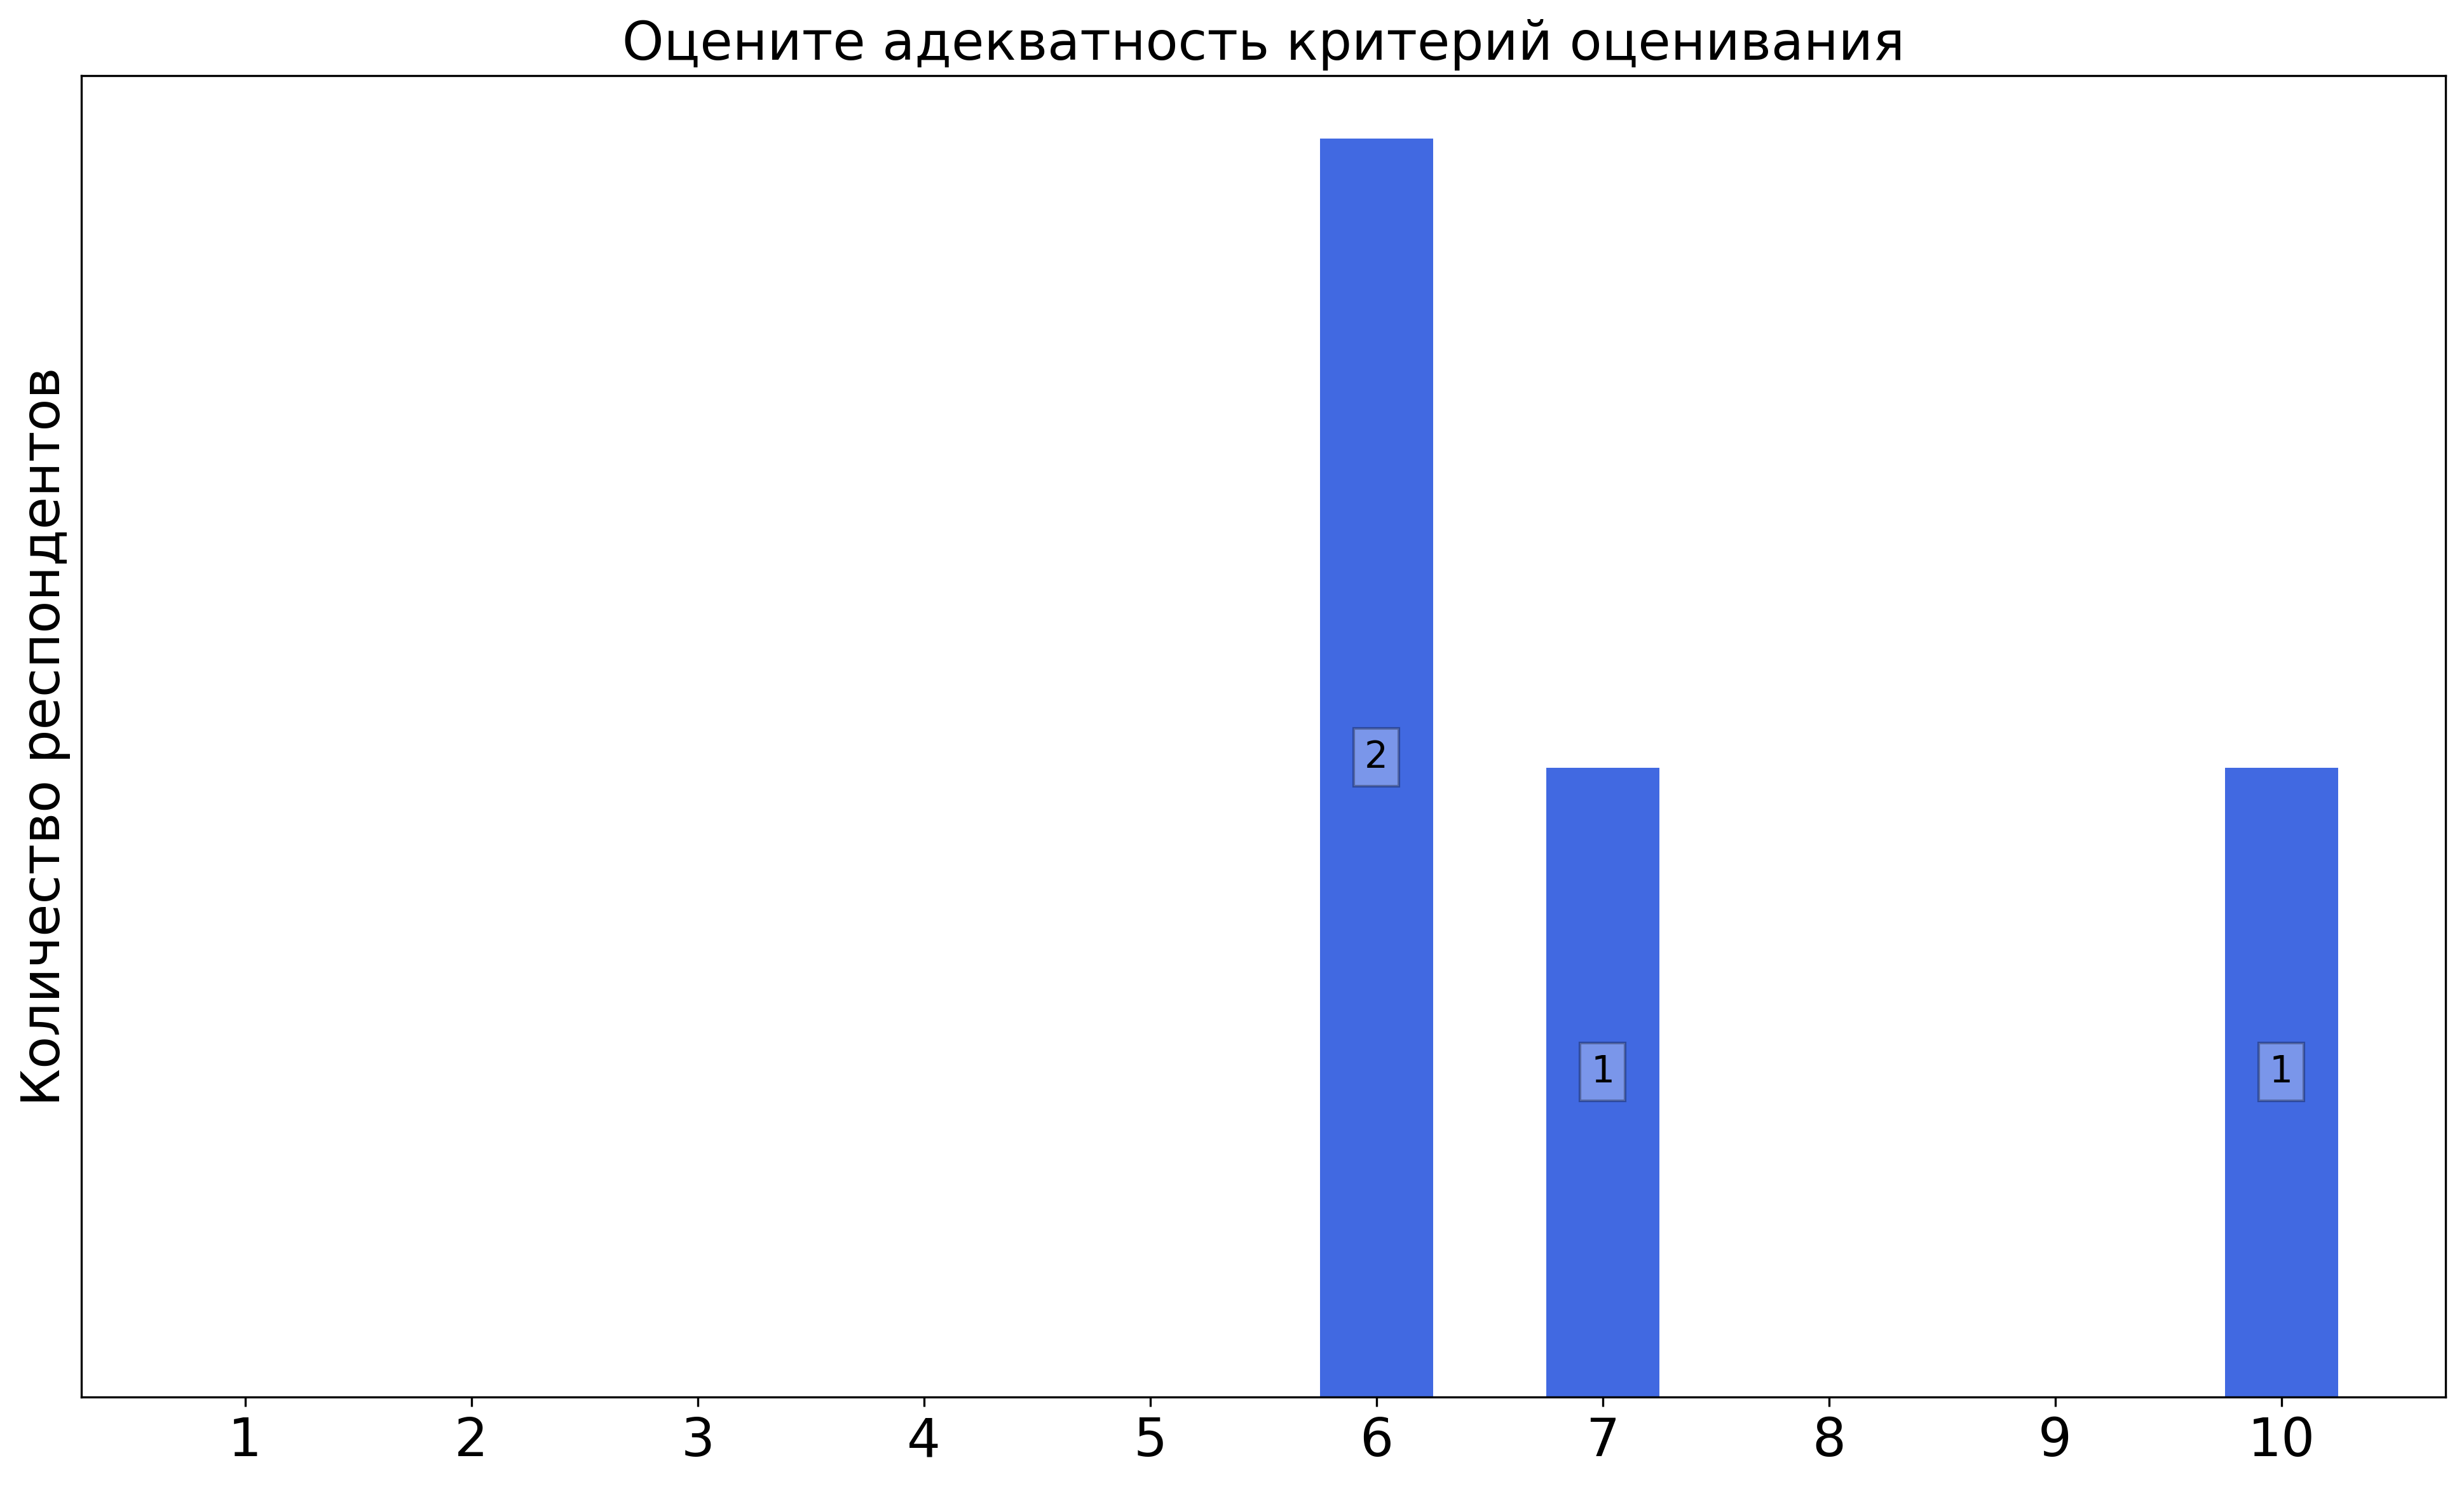
\includegraphics[width=\textwidth]{images/3 course/Вычислительная математика/seminarists-marks-Петров М.Н.-3.png}
			\end{subfigure}	
			\caption{Оценки респондентов о качестве преподавания семинаров}
		\end{figure}

		\textbf{Комментарии студентов о семинаристе\protect\footnote{сохранены оригинальные орфография и пунктуация}}
            \begin{commentbox} 
                Строгие правила, и мало практики, но это не плохо, так как основные темы достаточно примитивные и праки по ним это идейно "напишите свой стек на С". Задачки разбираются хорошо, домашка помогает закрепить материал, если у вас хорошая память, то предмет простой.
            \end{commentbox} 
        
            \begin{commentbox} 
                Семинары божеские, хорлшо объясняет, расшаривает каждому, кто не понял - буквально каждого обходит и спрашивает, как дела с задачкой, которую дал на семинаре. Но оценивает уж слишком жестко. Контрольную, которую я знал, как решать, я буквально написать не успел, и получил за нее мало баллов. 
            \end{commentbox} 
        
            \begin{commentbox} 
                Михаил Николаевич знает идеально свой предмет и отлично умеет его объяснять, но во время семестра пришлось очень много работать. Система оценивания очень строгая, но проверяет лояльно. Хотелось бы чуть снизить количество заданий, выполняемых в течение семестра, при этом сделать семинары, где студенты решают и обсуждают задачи, в особенности практические, это было бы очень интересно, познавательно, при этом увеличило бы знание предмета и навык обсуждать связанную с ним теорию и применять её на практике. 
            \end{commentbox} 
        
            \begin{commentbox} 
                тяжело, но очень круто 
            \end{commentbox} 


    \subsubsection{Отзыв студентов о семинарах. Семинарист: Фаворская А.В.}
		\begin{figure}[H]
			\centering
			\begin{subfigure}[b]{0.45\textwidth}
				\centering
				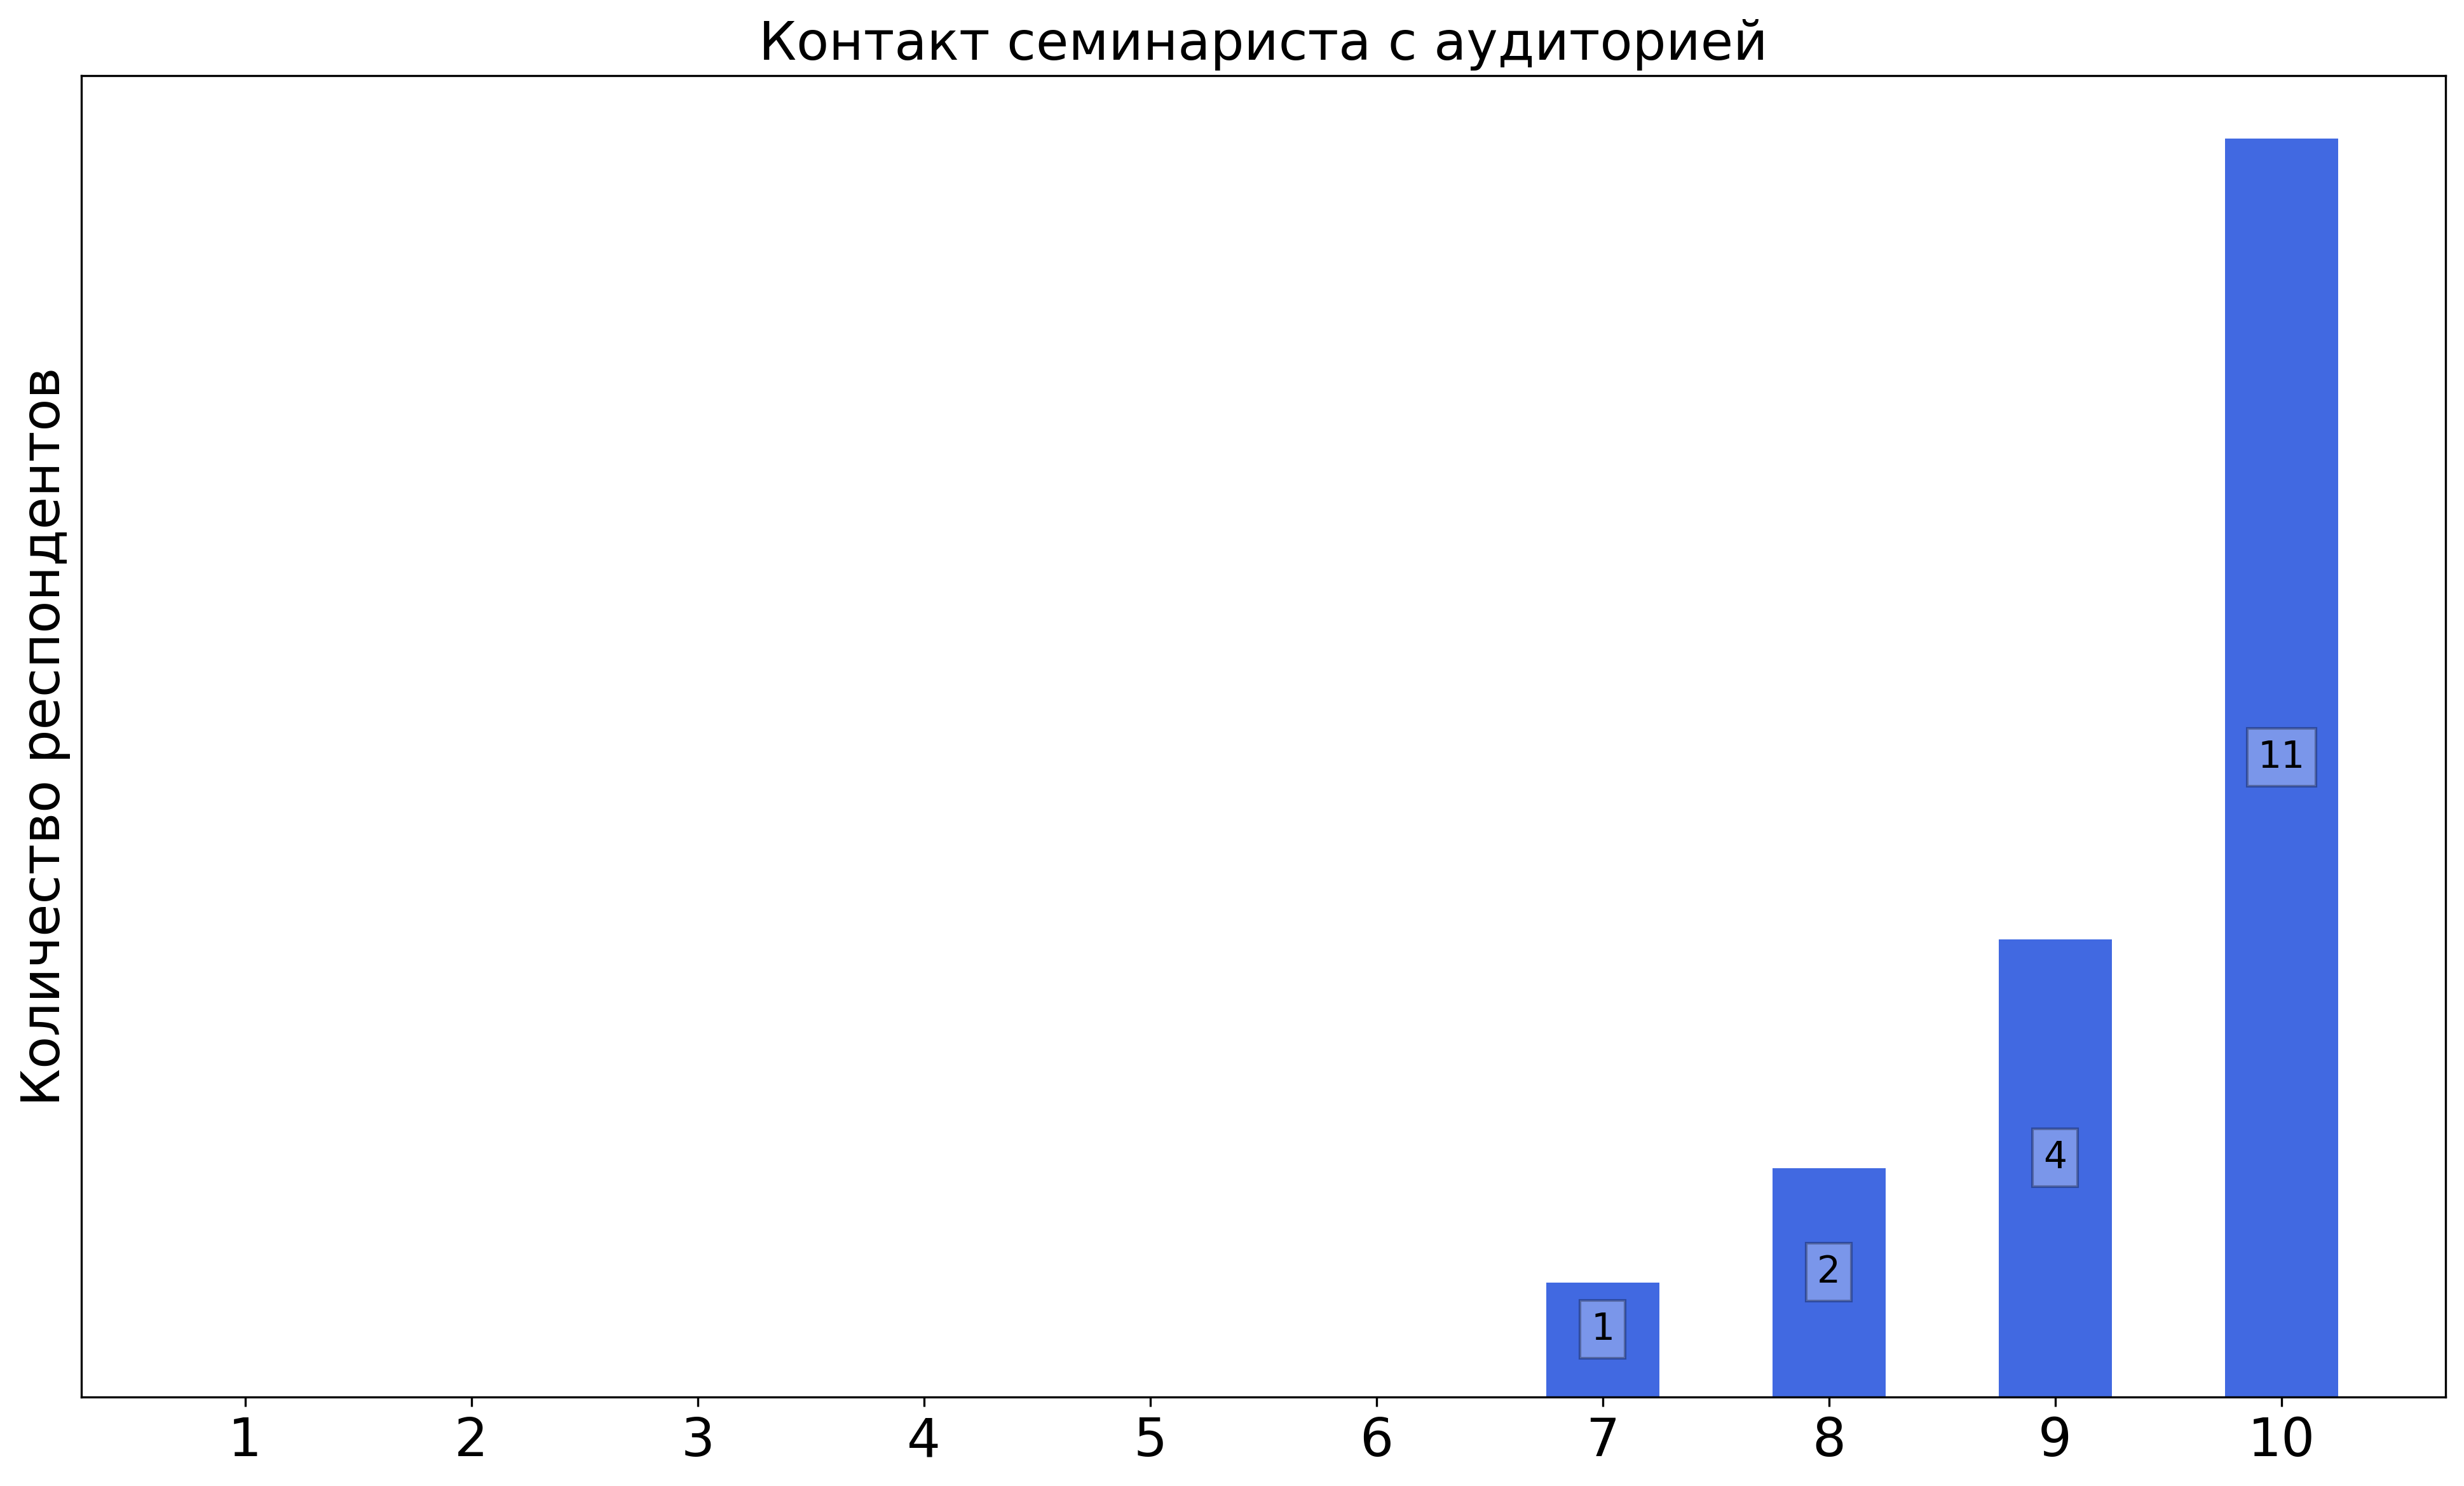
\includegraphics[width=\textwidth]{images/3 course/Вычислительная математика/seminarists-marks-Фаворская А.В.-0.png}
			\end{subfigure}
			\begin{subfigure}[b]{0.45\textwidth}
				\centering
				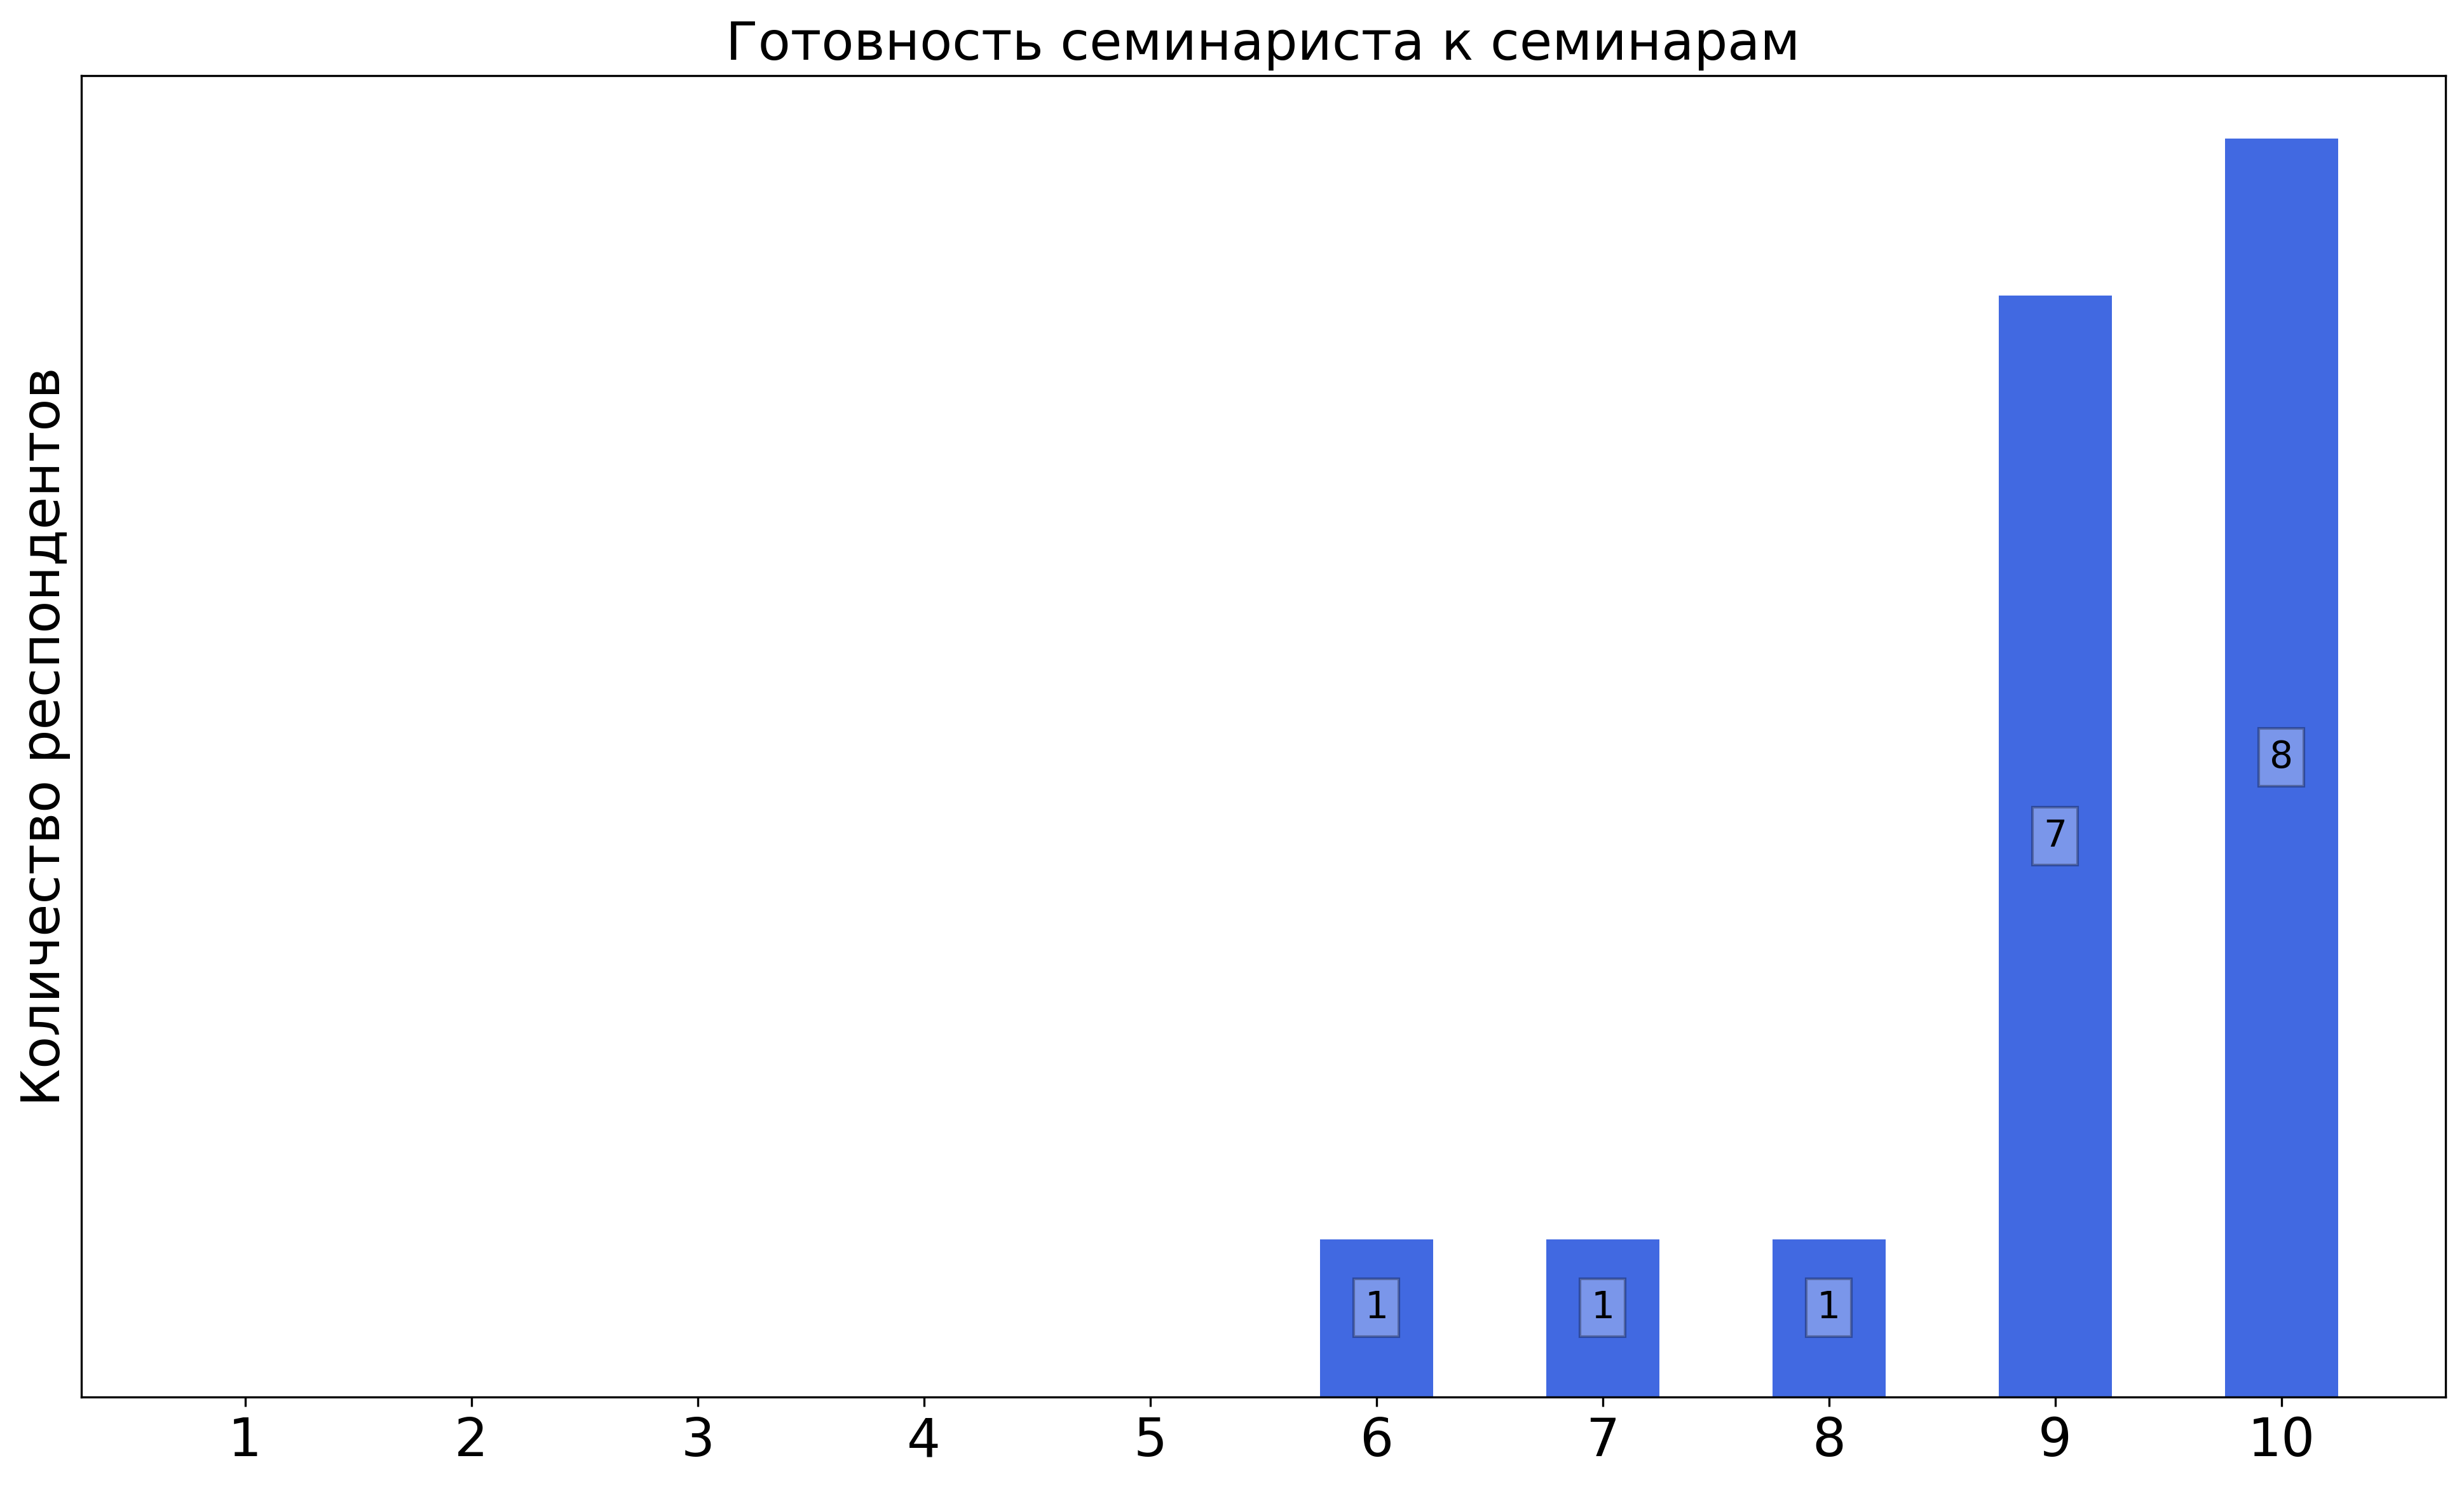
\includegraphics[width=\textwidth]{images/3 course/Вычислительная математика/seminarists-marks-Фаворская А.В.-1.png}
			\end{subfigure}
			\begin{subfigure}[b]{0.45\textwidth}
				\centering
				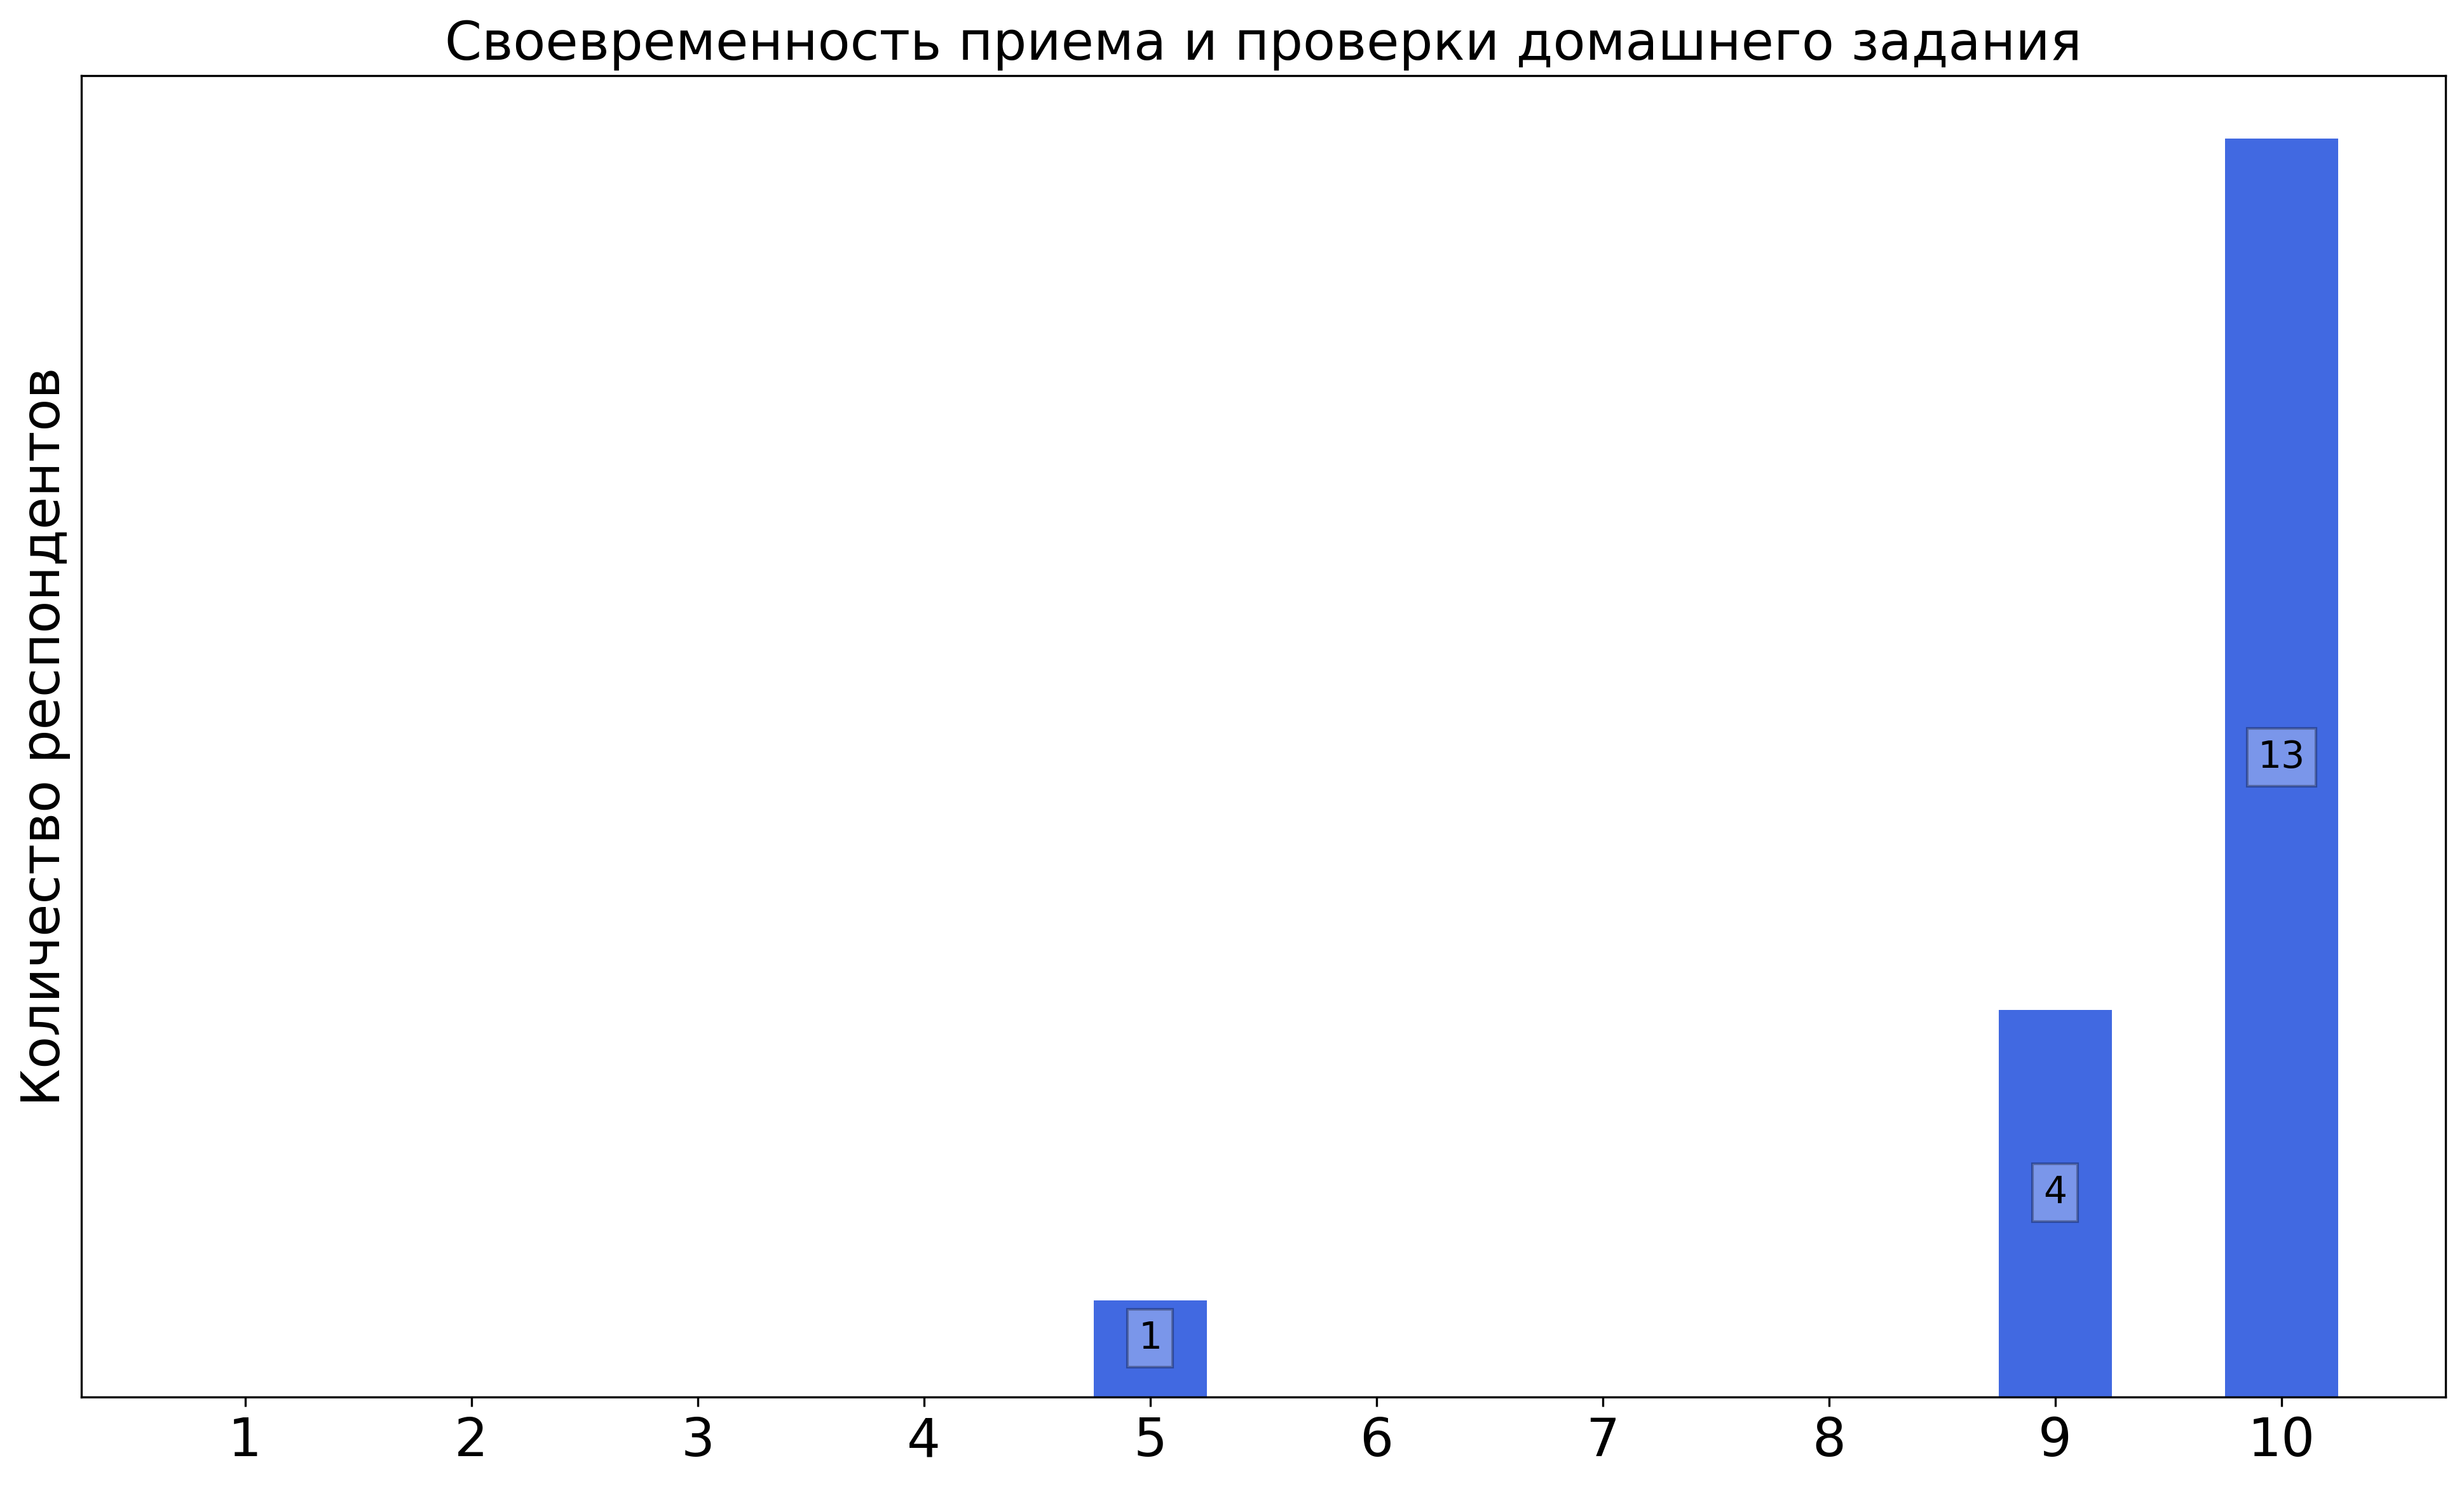
\includegraphics[width=\textwidth]{images/3 course/Вычислительная математика/seminarists-marks-Фаворская А.В.-2.png}
			\end{subfigure}
			\begin{subfigure}[b]{0.45\textwidth}
				\centering
				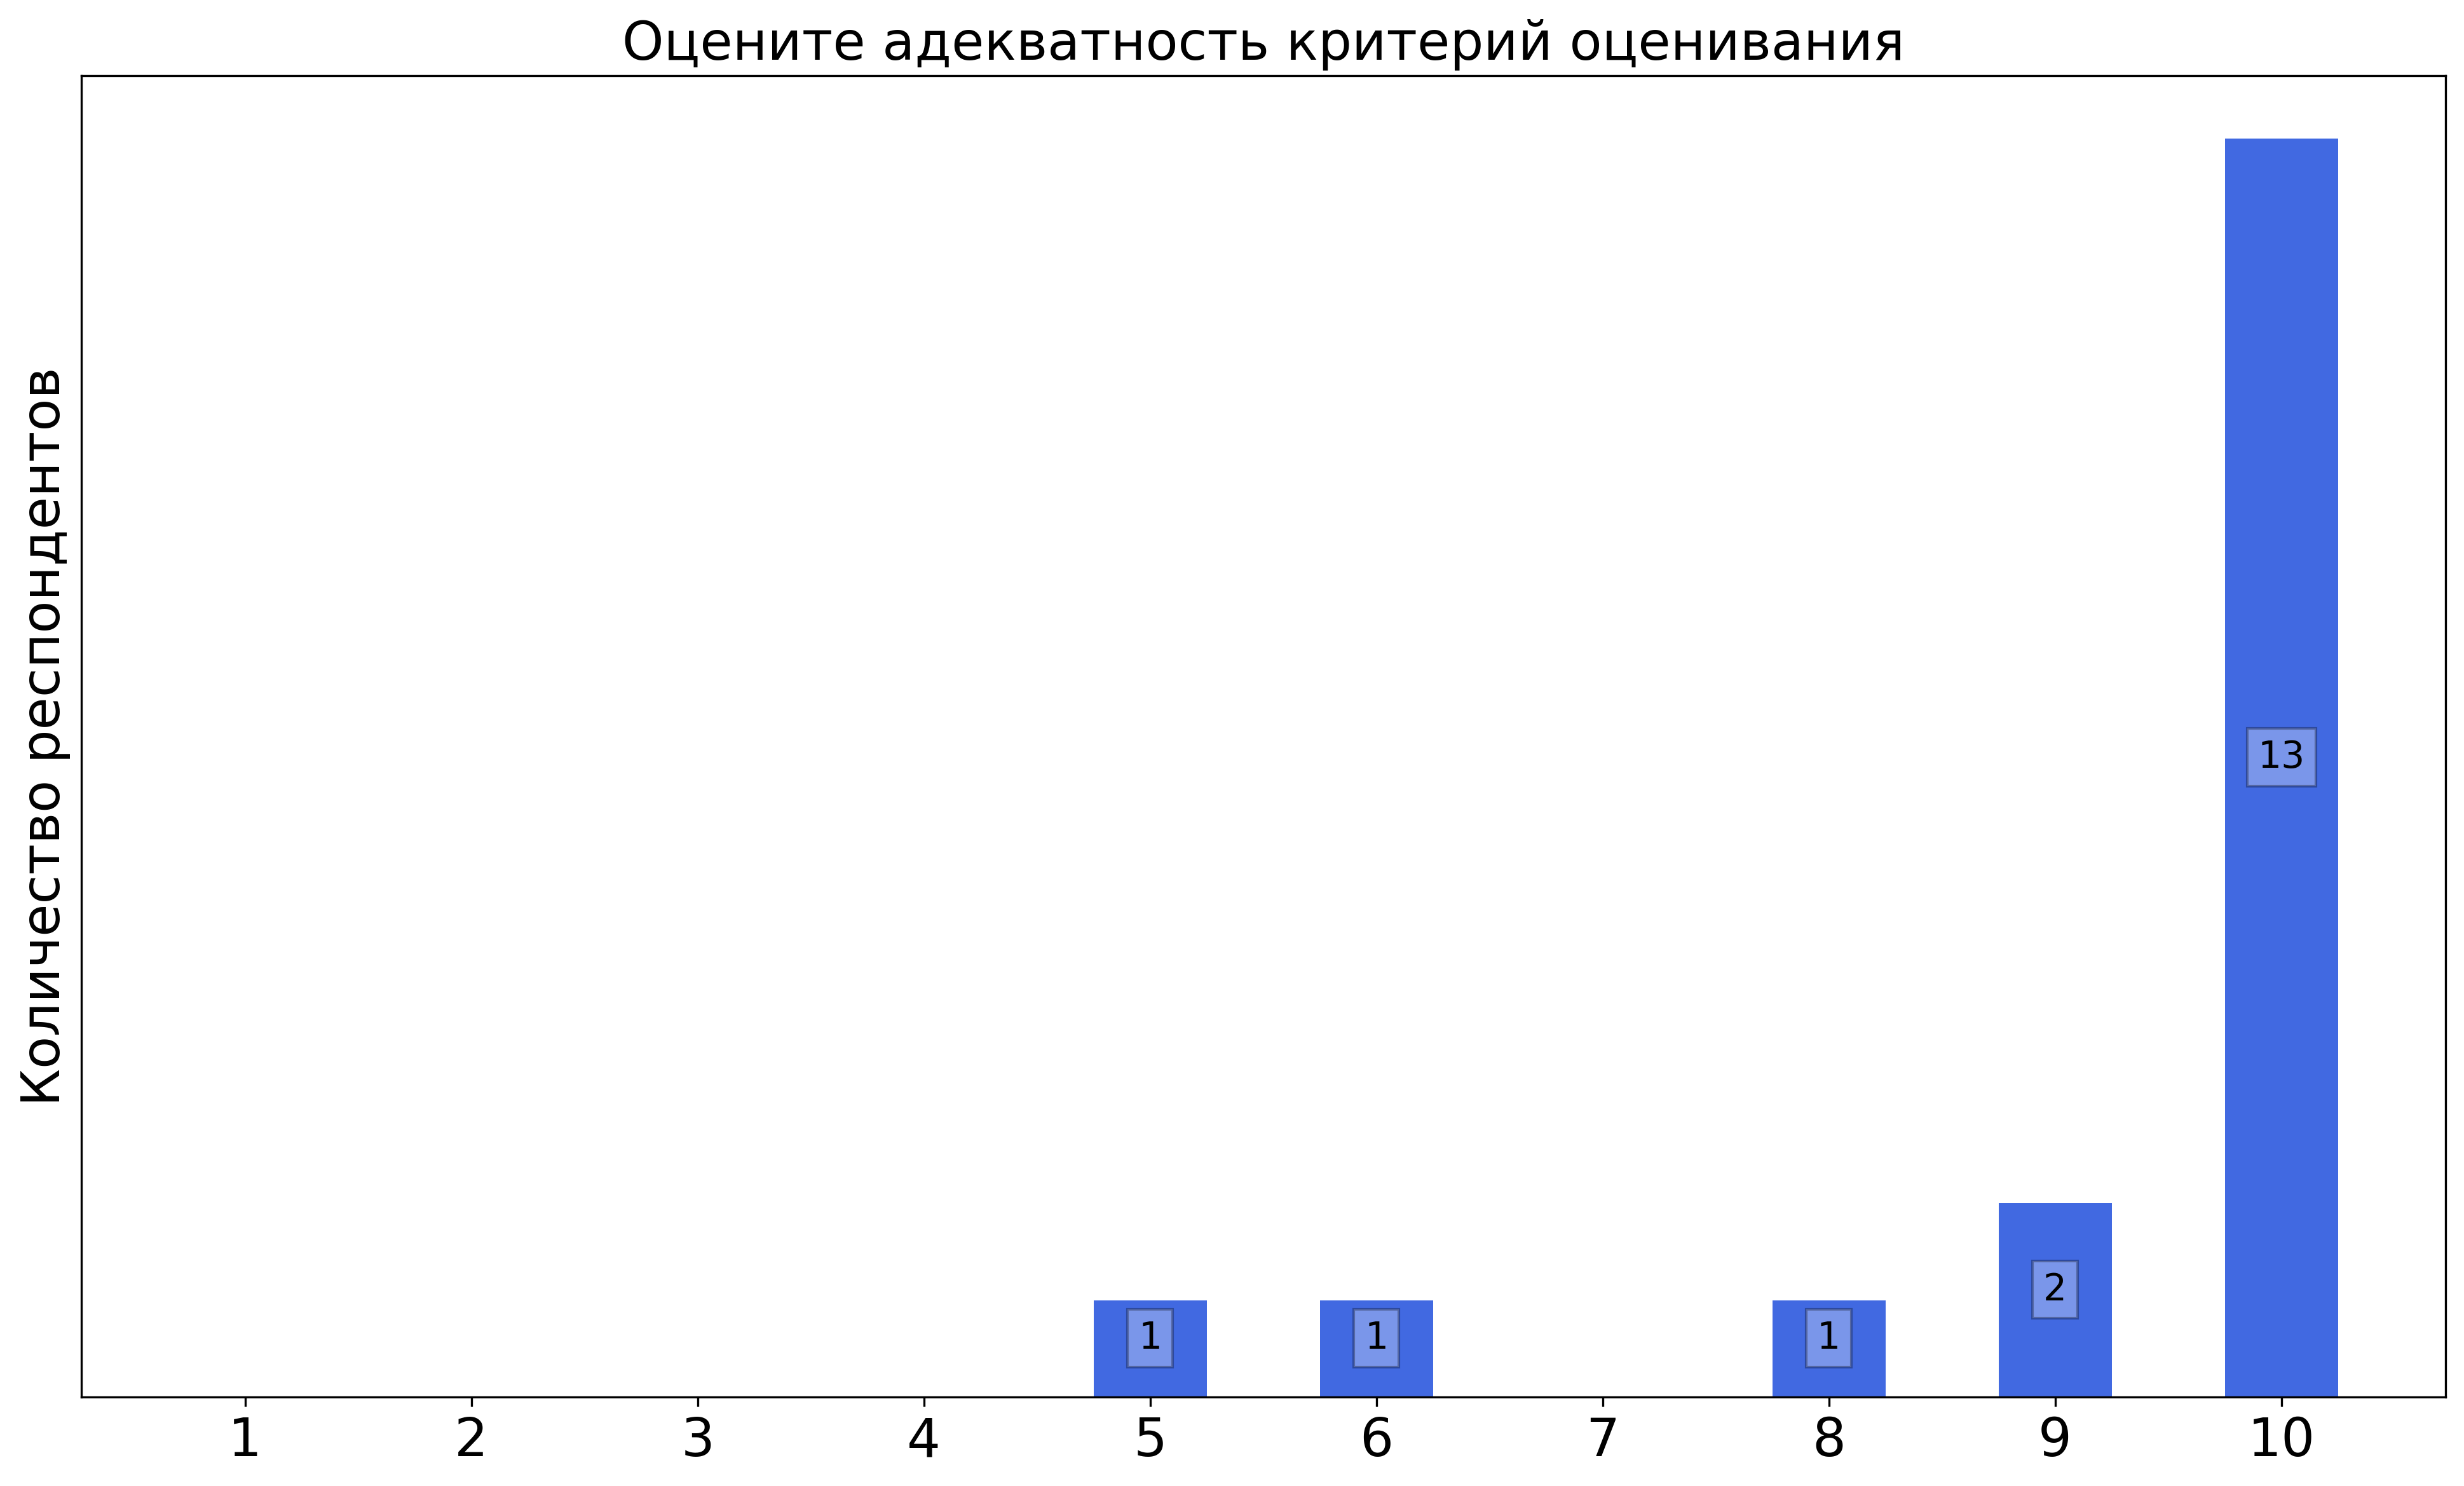
\includegraphics[width=\textwidth]{images/3 course/Вычислительная математика/seminarists-marks-Фаворская А.В.-3.png}
			\end{subfigure}	
			\caption{Оценки респондентов о качестве преподавания семинаров}
		\end{figure}

		\textbf{Комментарии студентов о семинаристе\protect\footnote{сохранены оригинальные орфография и пунктуация}}
            \begin{commentbox} 
                Классный семинарист, расшаривает, адекватное оценивание и контрольные. 
            \end{commentbox} 

            \begin{commentbox} 
                Одна из самых добрых преподавателей курса. При этом материал вроде бы был рассказан полностью (хотя может быть я не узнал всей глубины курса). Очень приятная в общении. Хотя есть ощущение, что я ничего с семинаров не вынес. (Но я не хотел бы чтобы она пропадала) 
            \end{commentbox} 

            \begin{commentbox} 
                Очень халявная, но объяснить может, невдаваясь в подробности 
            \end{commentbox} 

            \begin{commentbox} 
                Халява, если хочешь, то заботать вычматы можно. А если не хочешь, все равно отлично получить очень легко. 
            \end{commentbox} 

            \begin{commentbox} 
                Очень халявные семинары. При этом есть четкие критерии получения оценки (посещения, активность, контрольные). Домашние задания не обязательны (удос или даже хор можно получить и без них) 
            \end{commentbox} 

            \begin{commentbox} 
                Очень лояльно оценивает, можно даже не делать домашку. Для нормальной оценки надо часто выходить к доске, что помогает понять материал для контрольных 
            \end{commentbox} 

            \begin{commentbox} 
                Отличный семинарист, объясняет тему, отвечает на все вопросы, отлично разбирается. На контрольных разрешает пользоваться любыми материалами, благодаря чему получить хорошую оценку не проблема. Семинары проходят интересно и весело. 
            \end{commentbox}


    \subsubsection{Отзыв студентов о семинарах. Семинарист: Шильников К.Е.}
        \begin{figure}[H]
            \centering
            \begin{subfigure}[b]{0.45\textwidth}
                \centering
                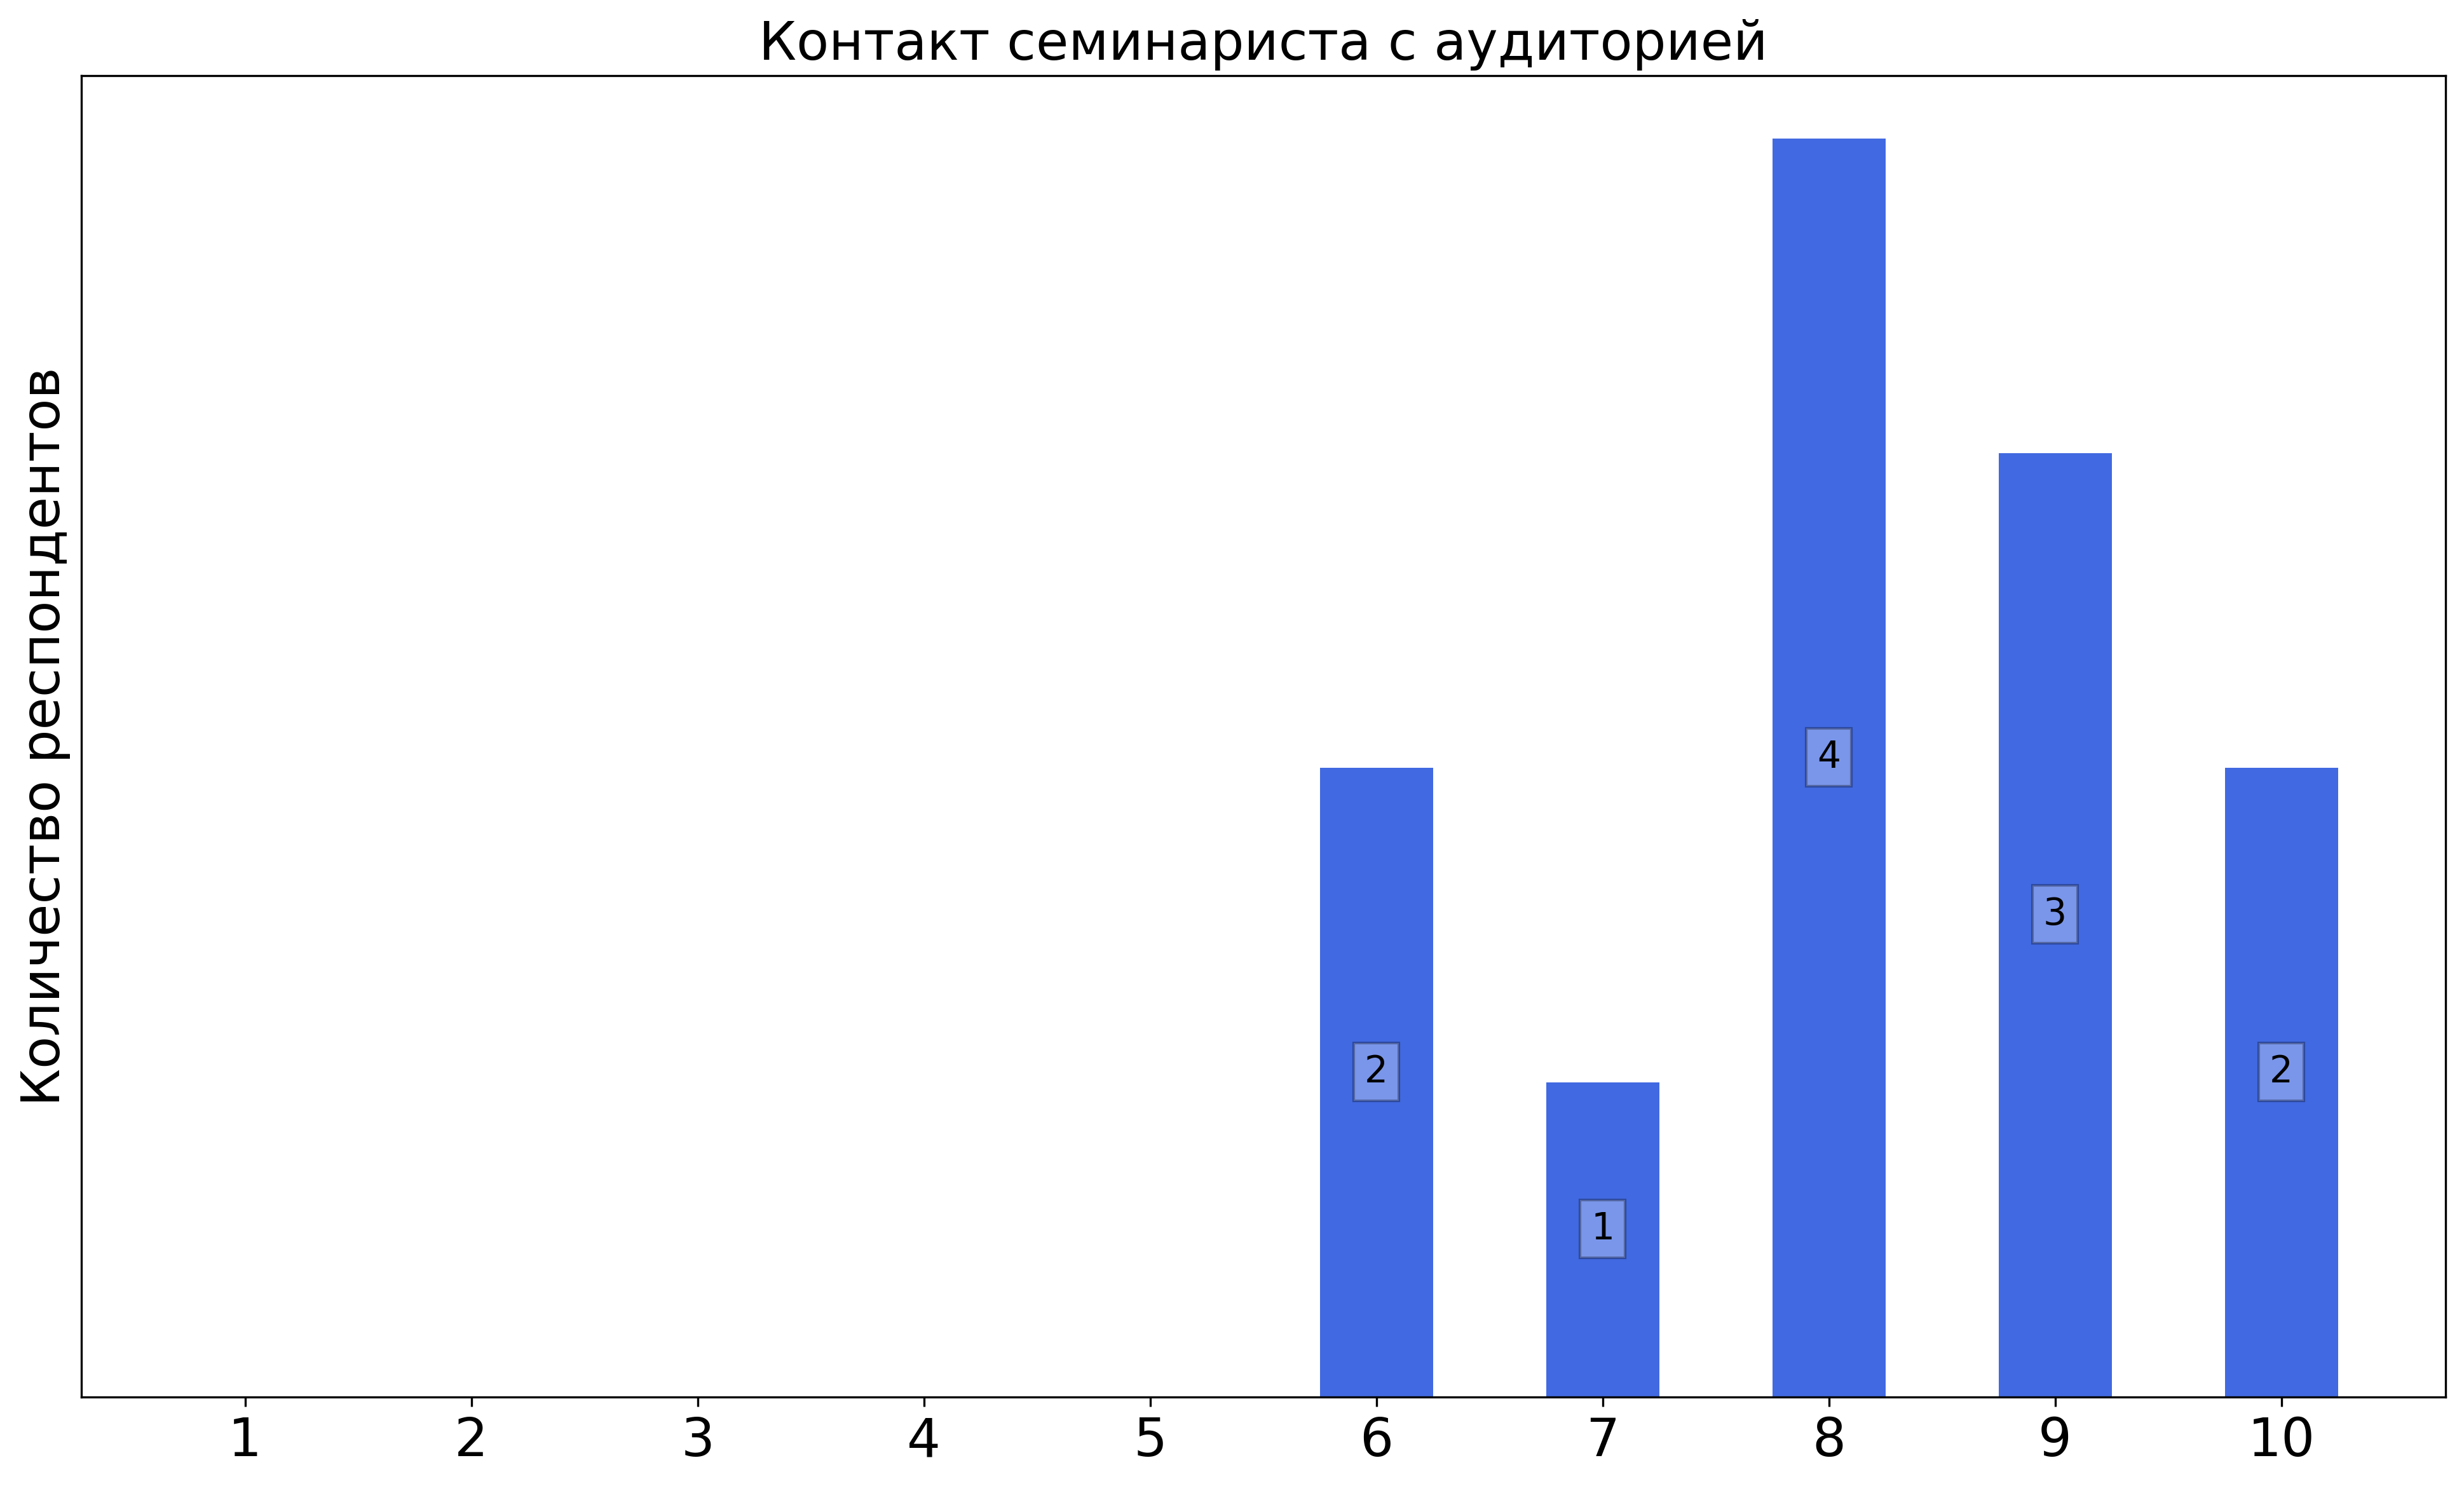
\includegraphics[width=\textwidth]{images/3 course/Вычислительная математика/seminarists-marks-Шильников К.Е.-0.png}
            \end{subfigure}
            \begin{subfigure}[b]{0.45\textwidth}
                \centering
                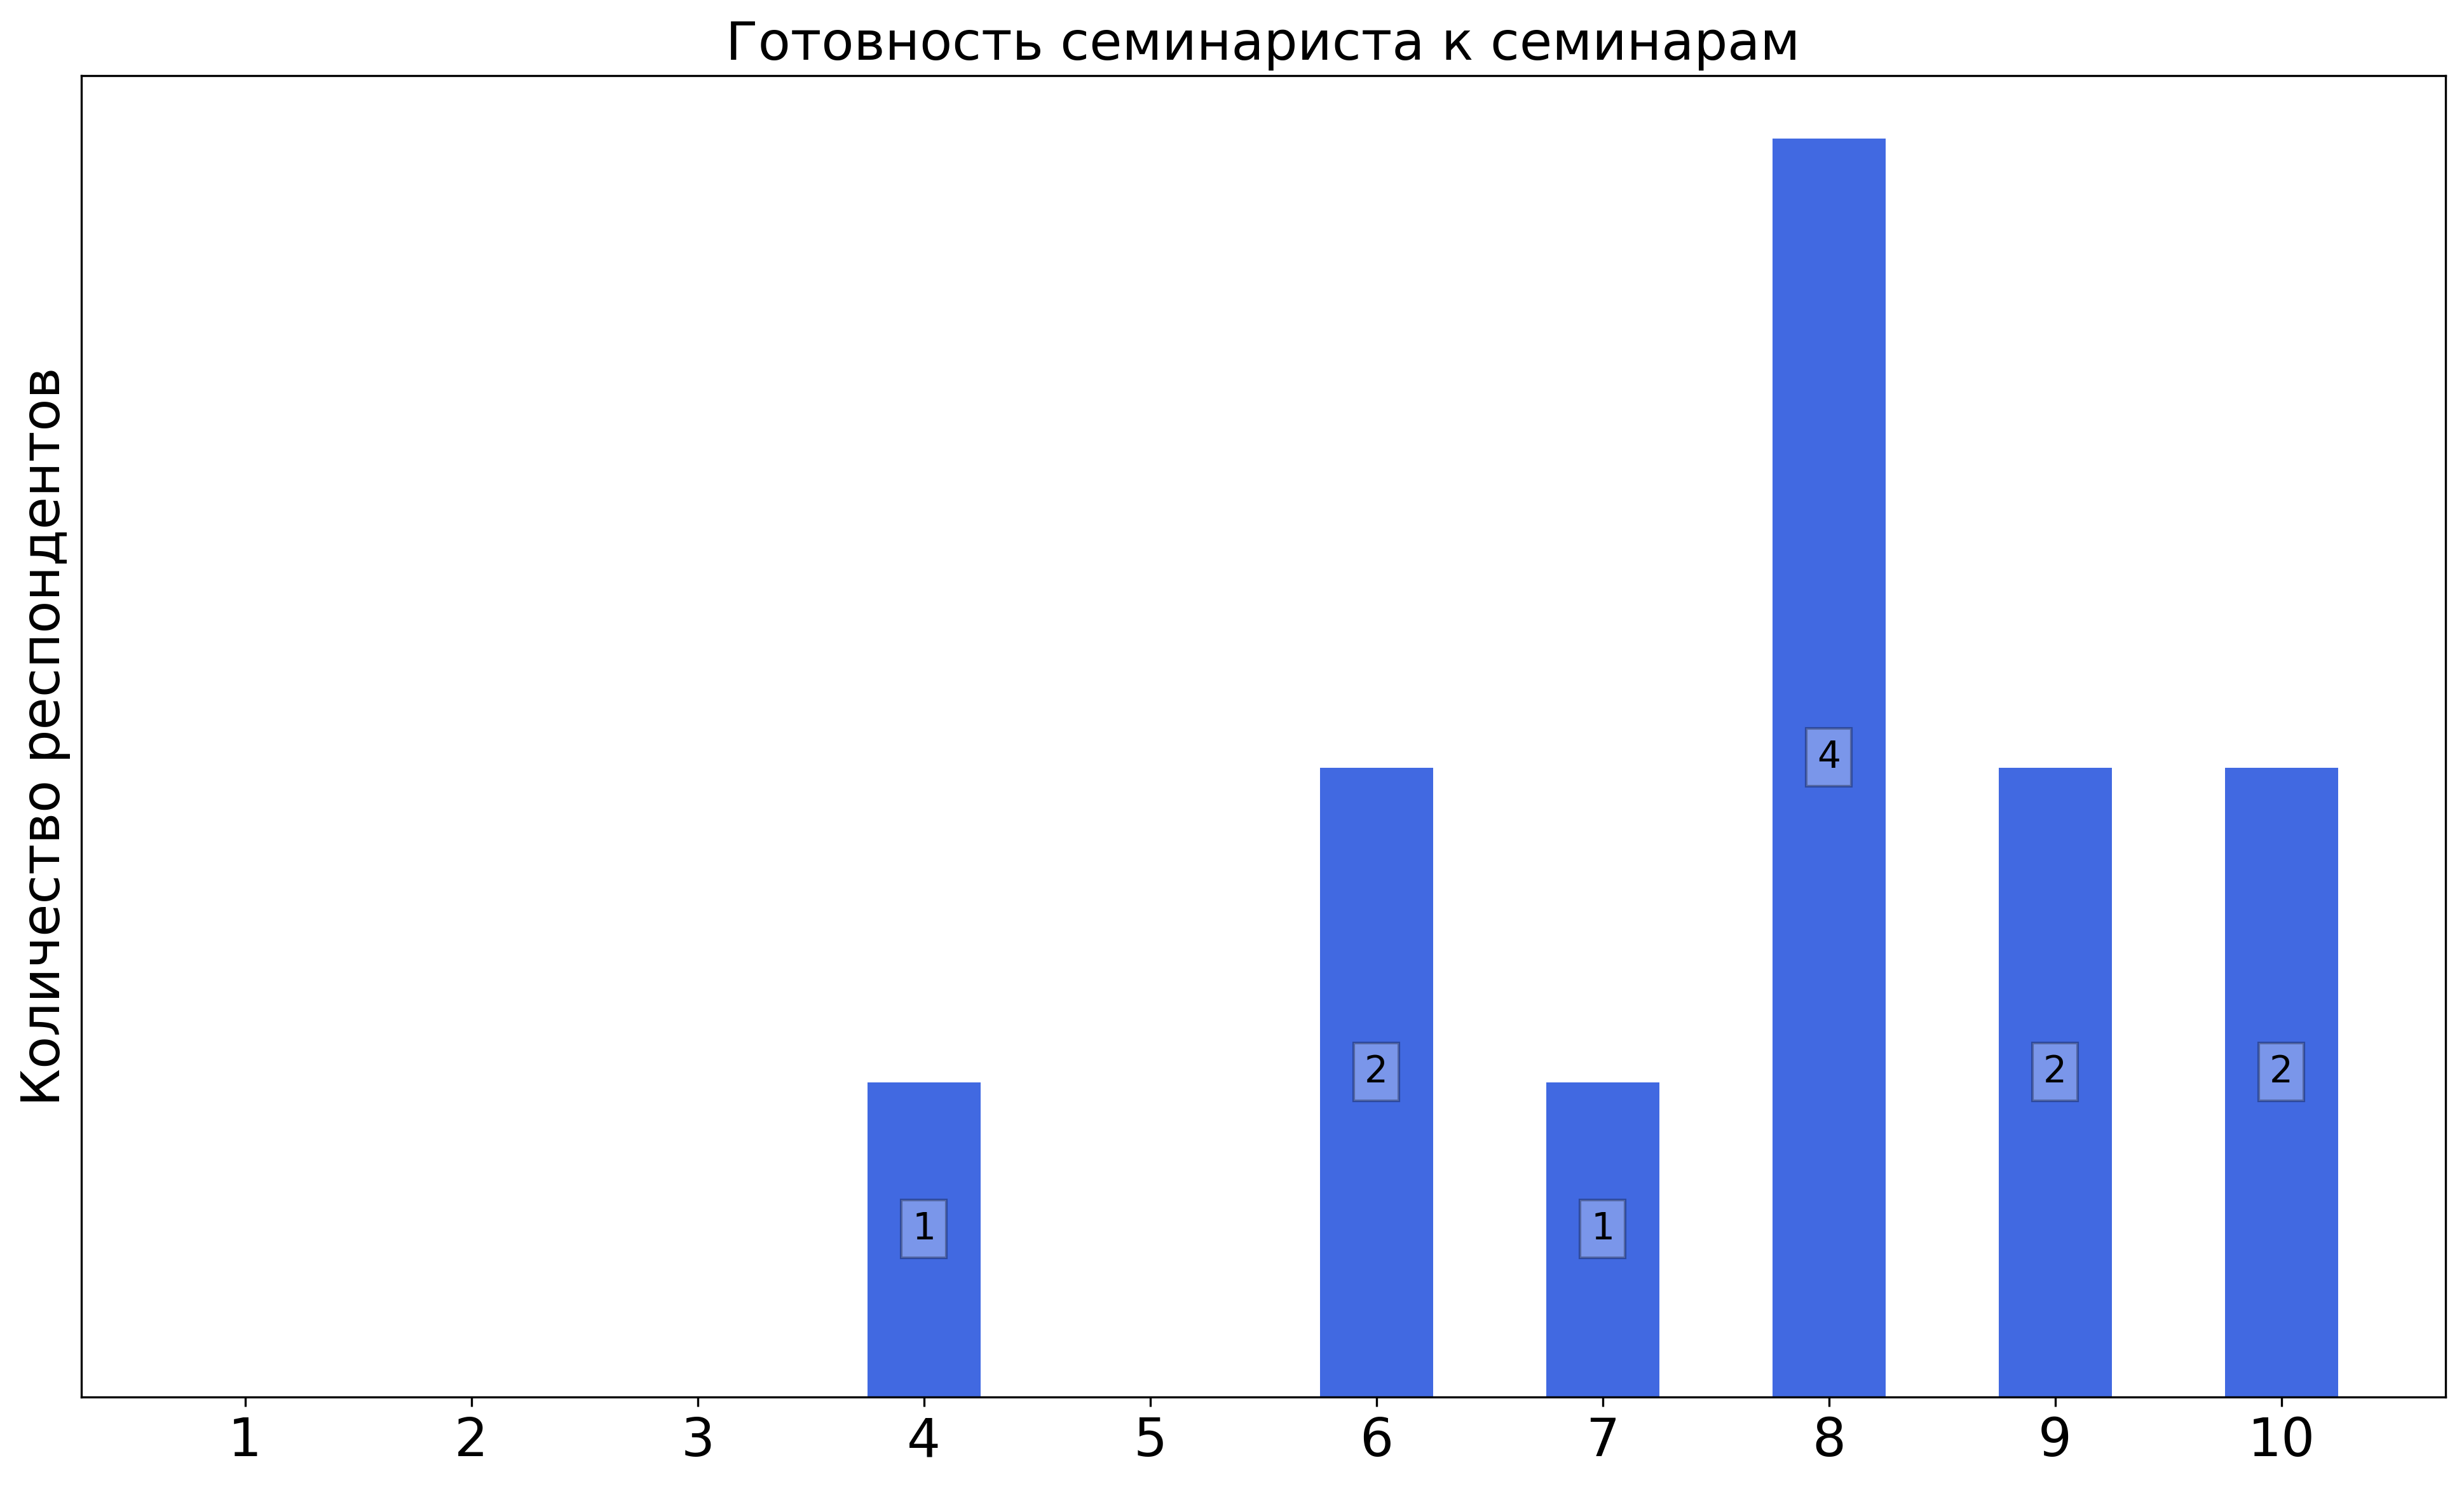
\includegraphics[width=\textwidth]{images/3 course/Вычислительная математика/seminarists-marks-Шильников К.Е.-1.png}
            \end{subfigure}
            \begin{subfigure}[b]{0.45\textwidth}
                \centering
                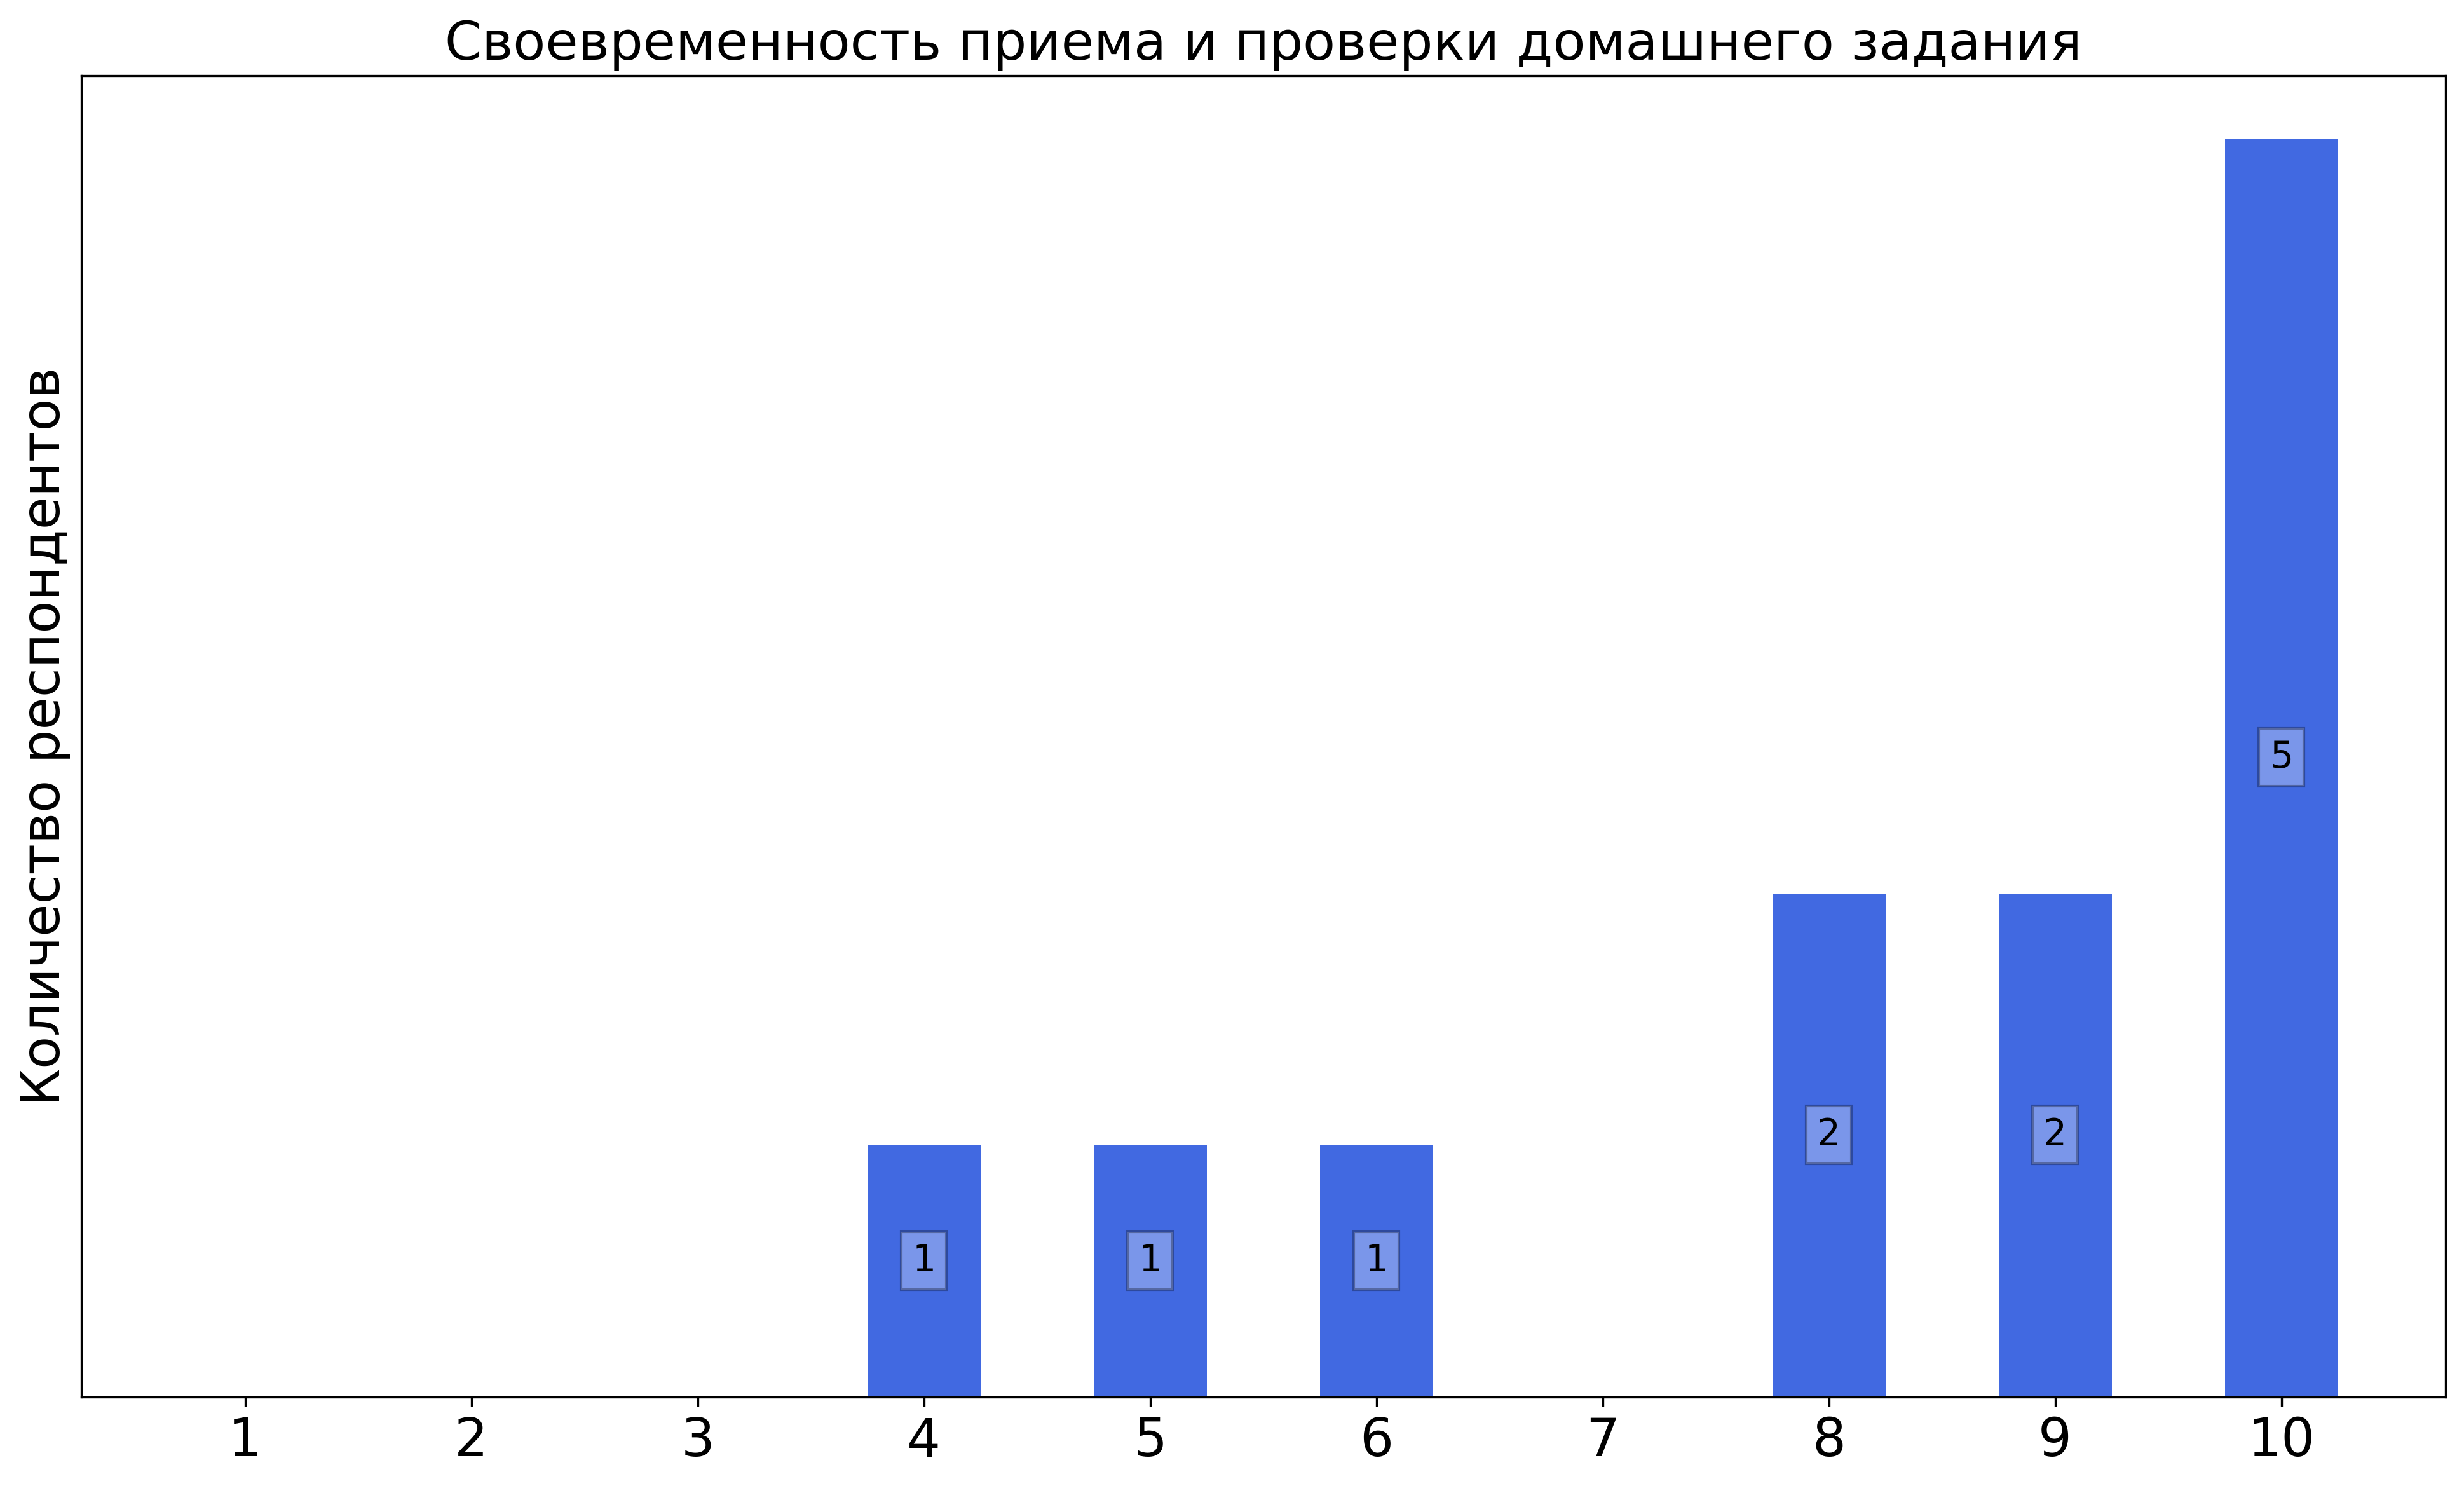
\includegraphics[width=\textwidth]{images/3 course/Вычислительная математика/seminarists-marks-Шильников К.Е.-2.png}
            \end{subfigure}
            \begin{subfigure}[b]{0.45\textwidth}
                \centering
                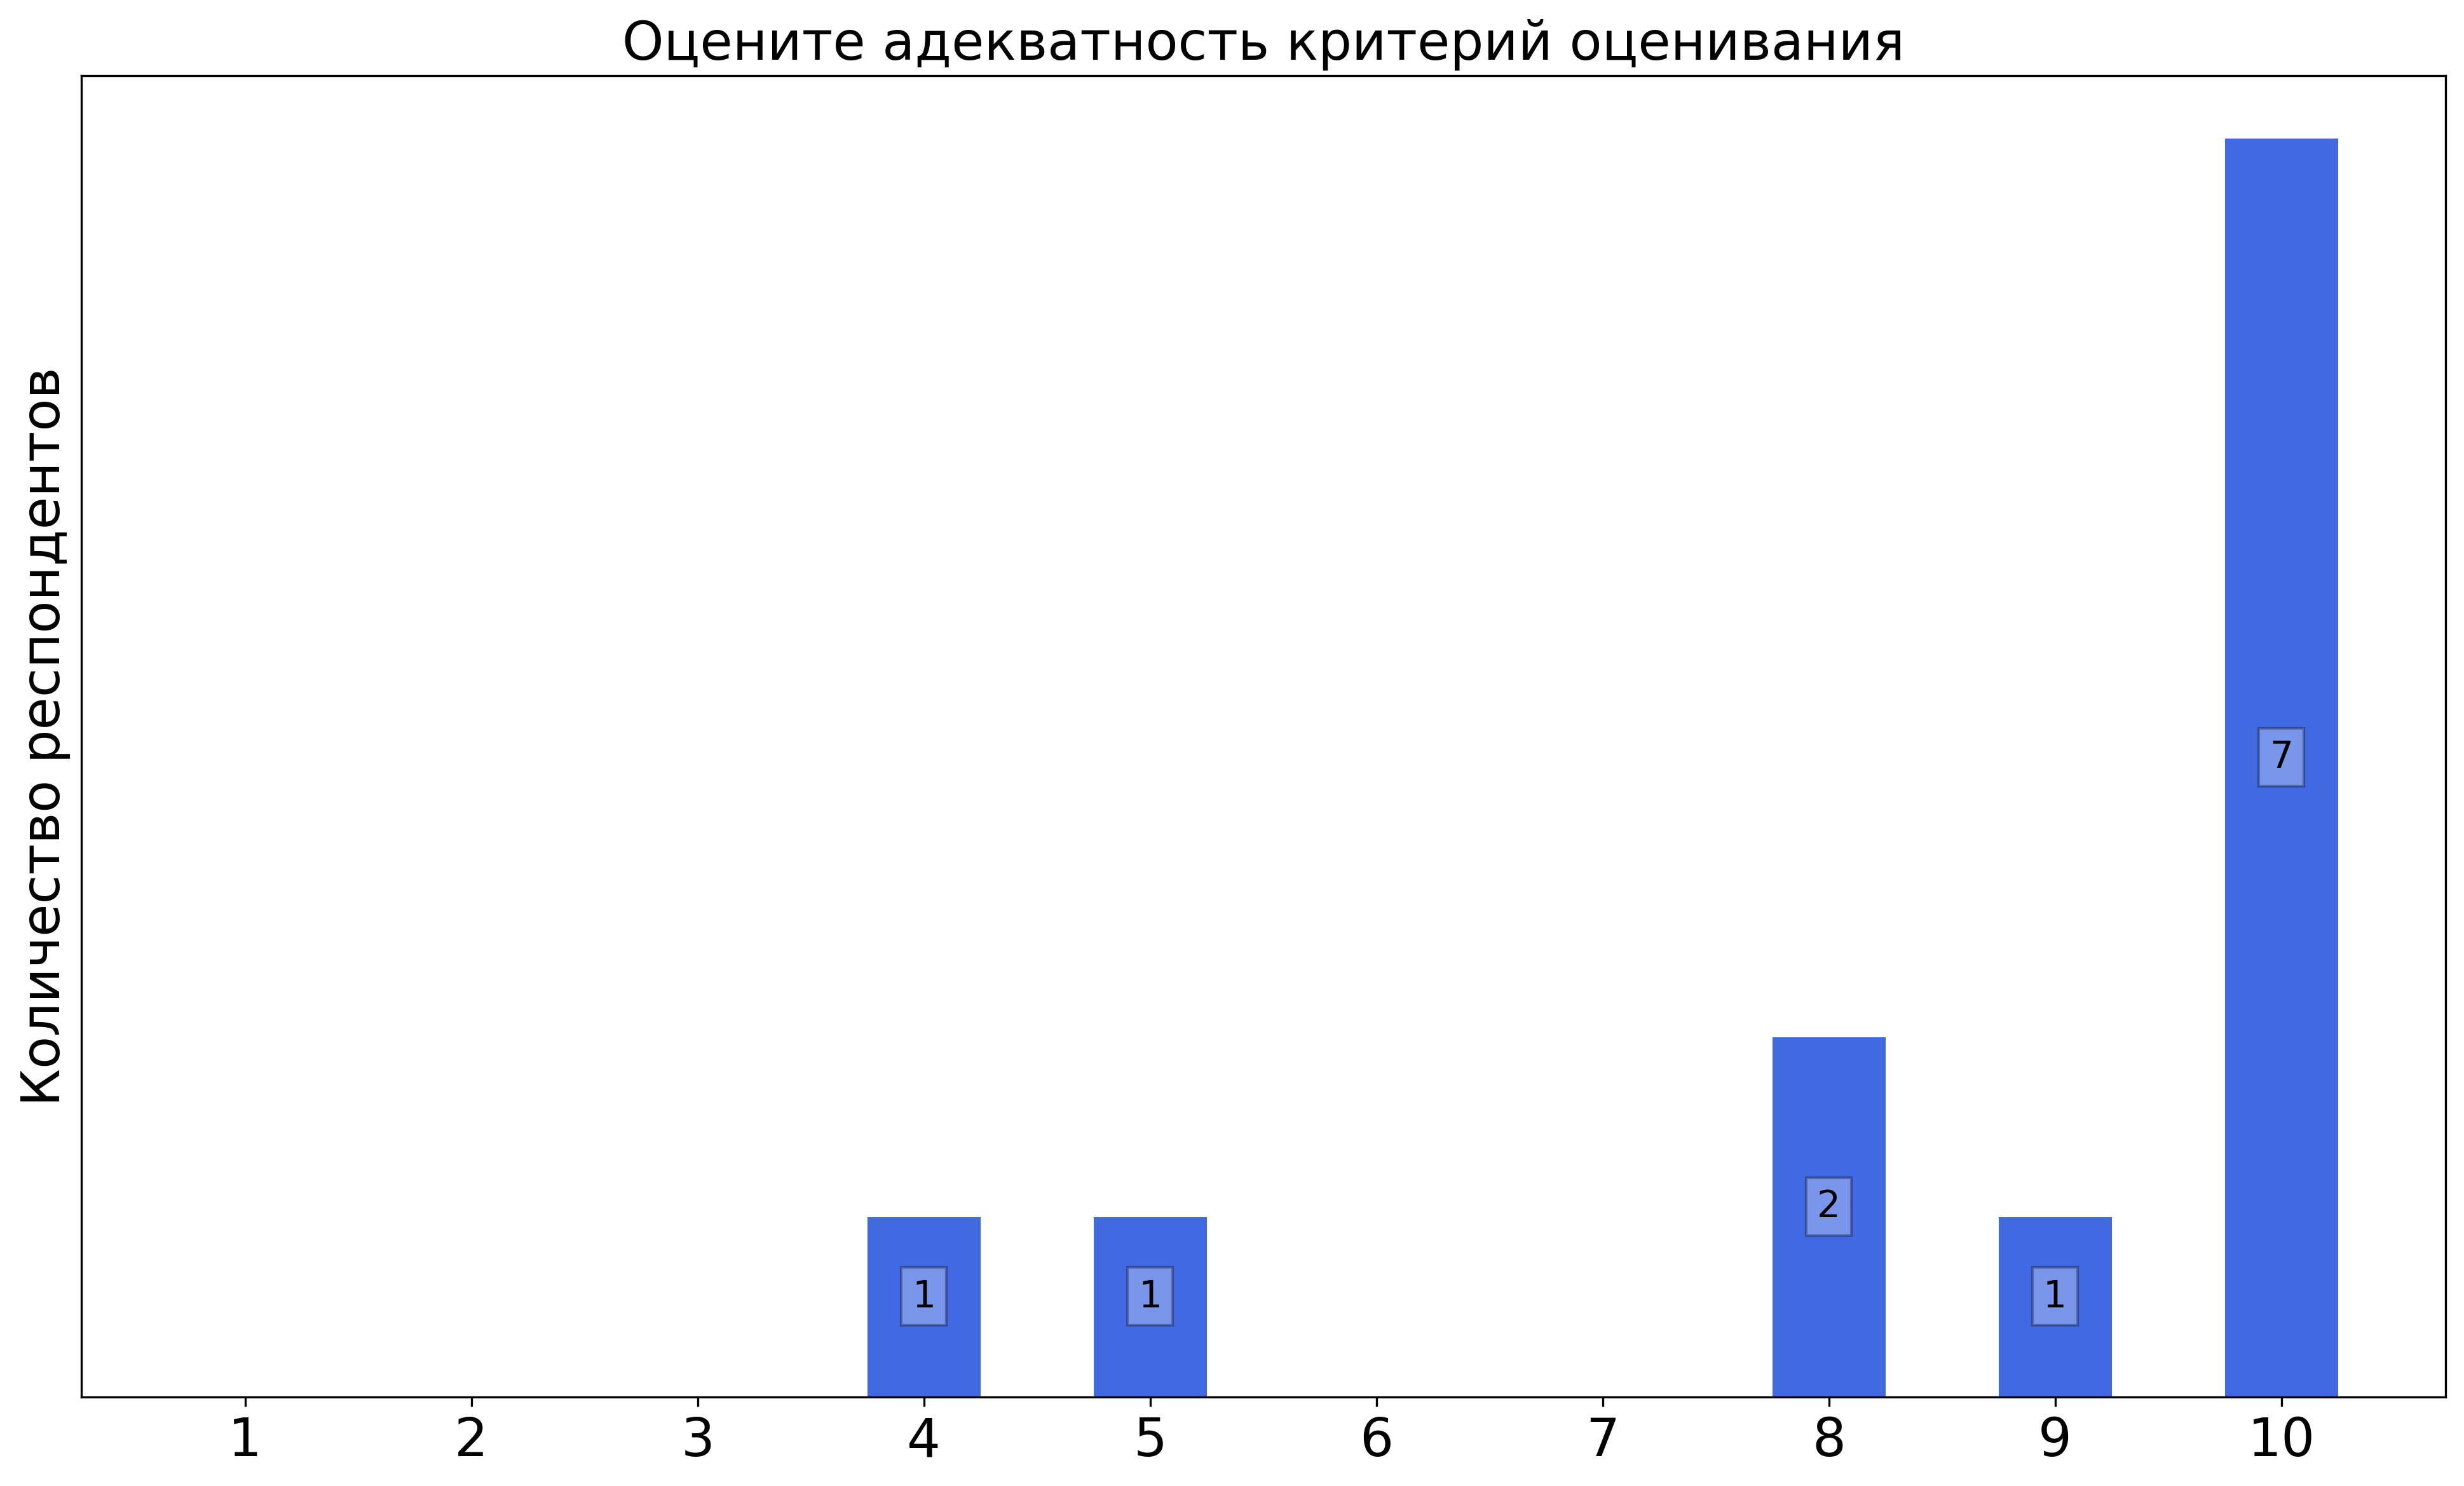
\includegraphics[width=\textwidth]{images/3 course/Вычислительная математика/seminarists-marks-Шильников К.Е.-3.png}
            \end{subfigure}	
            \caption{Оценки респондентов о качестве преподавания семинаров}
        \end{figure}

        \textbf{Комментарии студентов о семинаристе\protect\footnote{сохранены оригинальные орфография и пунктуация}}
            \begin{commentbox} 
                Семинарист рассказывает материал очень быстро, из-за чего записи скомканы. По приём лабораторных нет чётких сроков, что делает предмет весьма халявным. Иногда выводил что-то на семинарах, зависал и приходилось ждать, пока вспомнит, как решается задача 
            \end{commentbox} 
        
            \begin{commentbox} 
                Семинары были неплохие в первой половине курса, но ближе к концу возникло ощущение, что преподаватель плохо готовится к семинарам. Однако мне понравились его задания( лабораторные работы). Контрольные были не самыми сложными, оценивал адекватно 
            \end{commentbox} 
        
            \begin{commentbox} 
                Не было сформулированно четких критериев к лабам.  
            \end{commentbox} 
    
    \subsubsection{Прочие комментарии и предложения по улучшению курса}
        \begin{commentbox}
            Этот курс уже ближе к тому, что нам может пригодиться в жизни. Минусы - у каждого семинариста свои критерии, хотелось бы, чтобы они были у всех схожими
        \end{commentbox}

        \begin{commentbox}
            Непонятно, в чем цель курса, так как идеи за основными методами раскрываются слабовато, а сами по себе они в основном не применяются. То есть развивается какая-то общая вычматисткая логика, но очень поверхностно. Если углублять курс, то все темы покрыть не хватит времени, возможно, часть тем можно просто исключить.
        \end{commentbox}

        \begin{commentbox}
            Поставьте другого лектора. И не пускайте Фаворскую заменять лектора, этт еще больший ужас был
        \end{commentbox}

        \begin{commentbox}
            Хотелось бы видеть меньше теоретических задач и больше практических. Очень интересно было бы сделать проект в группе и обсудить его с другими студентами.
        \end{commentbox}

        \begin{commentbox}
            В курсе не хватает больше прикладных задач. Лично у нас на семинарах вообще было не обязательно написание программ, но это из-за того, что семинарист первый год. Предмет кажется прикольным, но сам курс както скучноват
        \end{commentbox}

        \begin{commentbox}
            Не давать на лекциях вводного материала вообще, чтобы не отбивать интерес у аудитории
        \end{commentbox}

        \begin{commentbox}
            Курс скучновато и очень растянут 
        \end{commentbox}

        \begin{commentbox}
            Либо увеличивать серьезность предмета, либо же убирать его вовсе. Лектору что-то сделать со структурой курса (ну он же видит, что к нему почти никто не ходит:( ), возможно писать на доске. Возможно стоит больше работать на компьютере на семинарах (мы этого не делали, хотя честно говоря нам давали выбор, но тут мб нужна палочная система).  В целом не почувствовал для себя практической пользы от предмета, хотя он вроде прикладной
        \end{commentbox}

        \begin{commentbox}
            Поменять формат лекций
        \end{commentbox}

        \begin{commentbox}
            Хотелось бы, чтоб лекции были структурированными, содержательными и , главное, - понятными. И чтобы выносить с них что-то, хотя бы конспект, а не недописанные отрезки отдельных фраз.
        \end{commentbox}

        \begin{commentbox}
            Надо пересмотреть преподавание предмета. Лекционный материал излишне затеоритизирован, отчего лекции практически никто не посещает, так как толку от них нет совсем.
        \end{commentbox}

        \begin{commentbox}
            Курс лекций очень оторван от практики и читается по презентациям, так что слушать его тяжело, да и практической пользы в этом не очень много. Курс семинаров Кожемяченко выстроен прекрасно, к нему вопросов нет.
        \end{commentbox}

        \begin{commentbox}
            Решения СЛАУ это конечно важно, но хочется чего-то более прикладного
        \end{commentbox}

        \begin{commentbox}
            Курс по некоторым причинам у большинства не входит в "топ" важных по приоритету уделяемого времени, поэтому не всегда хватает мотивации посещать занятия первой парой. Уверен, я бы погрузился глубже и освоил больше, если бы предмет проходил не первой парой.
        \end{commentbox}

        \begin{commentbox}
            Возможно сделать какой-то общий формат семинаров, потому что он очень разнится между группами - кто-то почти только прогает, у кого-то решение задач на доске и теория сплошная, плбс критерии выставления оценок тоже абсолютно индивидуальные у всех
        \end{commentbox}